\documentclass[11pt, a4paper, openright]{report}
%%
%% Package includes to provide the basic style
%%
\usepackage{graphicx}   % Permits import of various graphics formats
\graphicspath{{../img/}}
\usepackage{hyperref}   % Provides hyperlinks to sections automatically
\usepackage{pdflscape}  % Provides landscape mode for end code listings
\usepackage{multicol}   % Provides ability to split output into columns
\usepackage{listings}   % Provides styled code listings
\usepackage[left=3.5cm, right=2.5cm, top=3.5cm, bottom=3cm]{geometry} % Margins
\usepackage{titlesec}
\usepackage{lipsum}
\usepackage[numbers]{natbib}
\usepackage{enumerate}
\usepackage{tabularx}
\usepackage{longtable}
\usepackage{pgfgantt}
\usepackage{wrapfig}
\usepackage{amsmath, amsthm, amsfonts}
\newtheorem{definition}{Definition}
\usepackage{bbm}
\usepackage[shortlabels]{enumitem}
\usepackage{appendix}
\usepackage{todonotes}

\newcommand\requirement[2]{
  {#1} %\textbf{Priority: {#2}.}
}

\newcommand\invisiblesubsection[1]{
  \refstepcounter{subsection}
  \addcontentsline{toc}{subsection}{\protect\numberline{\thesubsection}#1}
  \subsectionmark{#1}}
\makeatother

\newcommand{\possessivecite}[1]{\citeauthor{#1}'s \citeyear{#1}}

  
%%
%% Set some page size changes from the standard article class
%%
\usepackage{calc}
\setlength{\parskip}{6pt}
\setlength{\parindent}{0pt}
\addtolength{\hoffset}{-0.5cm}
%\addtolength{\textwidth}{2.5cm}
\titleformat{\chapter}[display]{\vspace{-2cm}\normalfont\bfseries}{}{0pt}{\huge}

%%
%% Format definitions for the style
%%
%\usepackage{harvard}    % Uses harvard style referencing
\bibliographystyle{agsm}%{alpha}
\setcitestyle{authoryear}
%\citationstyle{dcu}
\pagestyle{headings}
\fussy



%%
%% Helpers
%% 
\usepackage[final]{pdfpages}
%\setcounter{secnumdepth}{4}


%%
%% Definitions to provide layout in the dissertation title pages
%%
\newenvironment{spaced}[1]
  {\begin{minipage}[c]{\textwidth}\vspace{#1}}
  {\end{minipage}}


\newenvironment{centrespaced}[2]
  {\begin{center}\begin{minipage}[c]{#1}\vspace{#2}}
  {\end{minipage}\end{center}}


\newcommand{\declaration}[2]{
  \thispagestyle{empty}
  \begin{spaced}{4em}
    \begin{center}
      \LARGE\textbf{#1}
    \end{center}
  \end{spaced}
  \begin{spaced}{3em}
    \begin{center}
      Submitted by: #2
    \end{center}
  \end{spaced}
  \begin{spaced}{5em}
    \section*{COPYRIGHT}

    Attention is drawn to the fact that copyright of this dissertation rests
    with its author. The Intellectual Property Rights of the products
    produced as part of the project belong to the author unless otherwise specified
    below, in accordance with the University of Bath's policy on intellectual property 
   (see http://www.bath.ac.uk/ordinances/22.pdf).

    This copy of the dissertation has been supplied on condition that anyone
    who consults it is understood to recognise that its copyright rests with its
    author and that no quotation from the dissertation and no information
    derived from it may be published without the prior written consent of
    the author.

    \section*{Declaration}
    This dissertation is submitted to the University of Bath in accordance
    with the requirements of the degree of Bachelor of Science in the
    Department of Computer Science. No portion of the work in this dissertation
    has been submitted in support of an application for any other degree
    or qualification of this or any other university or institution of learning.
    Except where specifically acknowledged, it is the work of the author.
  \end{spaced}

  \begin{spaced}{5em}
    Signed: \vspace{1cm}
\includegraphics[width=3cm]{img/signature.png}
  \end{spaced}}
  



\newcommand{\consultation}[1]{%
\thispagestyle{empty}
\begin{centrespaced}{0.8\textwidth}{0.4\textheight}
\ifnum #1 = 0
This dissertation may be made available for consultation within the
University Library and may be photocopied or lent to other libraries
for the purposes of consultation.
\else
This dissertation may not be consulted, photocopied or lent to other
libraries without the permission of the author for #1 
\ifnum #1 = 1
year
\else
years
\fi
from the date of submission of the dissertation.
\fi
\vspace{4em}

Signed: 
\includegraphics[width=3cm]{img/signature.png}
\end{centrespaced}
}


\usepackage{epigraph}
%\epigraphsize{\small}
\setlength\epigraphwidth{13cm}
\setlength\epigraphrule{0pt}

\usepackage{etoolbox}

\makeatletter
\patchcmd{\epigraph}{\@epitext{#1}}{\itshape\@epitext{#1}}{}{}
\makeatother


%%
%% END OF DEFINITIONS
%%



\title{\Huge\textbf{Mind The Gap:\\Newsfeed Visualisation\\with Metro Maps}}
\author{Damask Talary-Brown}
\date{Bachelor of Science in Computer Science with Honours\\The University of Bath\\ \the\year}

\begin{document}


\setcounter{page}{0}
\pagenumbering{roman}
\maketitle
\newpage

\consultation{0}
\newpage

\declaration{Mind The Gap: Newsfeed Visualisation with Metro Maps}{Damask Talary-Brown}
\newpage

\abstract
\addcontentsline{toc}{chapter}{Abstract}
\newpage
\tableofcontents
\newpage
\listoffigures
\addcontentsline{toc}{chapter}{List of Figures}
\listofalgorithms
\addtocontents{loa}{\def\string\figurename{Algorithm}}
%\newpage
%\listoftables
%\addcontentsline{toc}{chapter}{List of Tables}
%\newpage
%\chapter*{Acknowledgements}
%\addcontentsline{toc}{chapter}{Acknowledgements}
\newpage

\setcounter{page}{1}
\pagenumbering{arabic}

\chapter*{Introduction}
\addcontentsline{toc}{chapter}{Introduction}
\vspace{-0.5cm}
\epigraph{``The Press, Watson, is a most valuable institution, if you only know how to use it."}{--- \textup{Sherlock Holmes}, The Adventure of the Six Napoleons\\[0.2cm] \textup{Sir Arthur Conan Doyle}}

\section*{Why don't we Understand the News?}

The day the result of the 2016 United Kingdom EU Membership Referendum was announced, the \citeauthor{googletrends} reported a 250\% increase in searches for ``What happens if we leave the EU?'' Much like the case of David Leonhardt's 2008 article in the New York Times which began, ``Raise your hand if you don't quite understand this whole financial crisis,'' national news commentary had focused on little else in the preceding months.

Some months after Leonhardt's article was published, Journalism Professor Jay Rosen voiced his agreement with its premise in a blog post on the failure of journalism during the financial crisis; ``there are certain very important stories -- and the mortgage crisis is a good example -- where until I grasp the whole I am unable to make sense of any part.''\citep{NationalExplainer}

Studies have found that the general public use news media to make important life decisions, for entertainment and discussion, as a requirement of their jobs, and out of perceived civic obligation \citep{InformationCartography,UnderstandingTheParticipatoryNewsConsumer}. As a result of the ongoing shift towards online multimedia journalism, there has been an explosion of globally accessible knowledge which is expanding at an unprecedented rate as the internet grows. 

Although ubiquitous news media has resulted in more immediate and diverse coverage of current events, the volume of content available online has made the process of understanding it both daunting and off-putting to young adults \citep{anewmodelfornews}. Additionally, while news aggregators and RSS readers make it faster for users to access the news they care about, they do not aid comprehension. In spite of these facts, little attention has been given to addressing the problem that understanding news articles individually is inherently reliant on understanding news articles as a collection. 

Existing information infrastructure has been criticised both for not supporting the cross-correlation between collections of related news articles \citep{GalaxyOfNews}, and for attempting fit complex narratives into reductive and misleading visualisations \citep{InformationCartography}. Research into how humans' spatio-cognitive abilities can be applied to more abstract visual metaphors \citep{FromMetaphorToMethod} suggests the strength of visual metaphors lies in their familiarity. We therefore build on the work of \cite{GeneratingInformationMaps} to integrate the Metro Map metaphor into the news aggregation process.

\section*{Key Aims and Contributions}
The primary aim of this project is the development of a tool which generates interactive metro maps of news from RSS feeds, with individual articles transformed into stations and common themes transformed into \textit{metro lines}. Our goal is to reduce the information overload experienced by news consumers by providing contextual links between articles and topics.

The resultant system is a news feed aggregator with graphically structured output, and to the best of our knowledge is first of its kind. Contributions of this dissertation include:\vspace{-0.3cm}
\begin{itemize}[itemsep=0.1em]
	\item Implementation of efficient keyword extraction using tf-idf \citep{tfidf} on a reduced keyword space of named entities (Section \ref{sec:keys}).
	\item A novel and lightweight method for performing entity disambiguation within current events articles using Google's Knowledge Graph API (Section \ref{sec:gkg}).
	\item Formalisation of the metrics \textit{Line Coverage} and \textit{Affinity} as criteria for evaluating and ranking candidate metro lines (Sections \ref{sec:linecoverage} and \ref{sec:affinity}).
	\item Recommendations for how D3.js parameters can be manually tuned to generate initial force-directed station positions for planar embeddings of metro maps (Section \ref{sec:fdp}).
	\item The first application of \citeauthor{AutomaticMetroMapLayoutThesis}'s [\citeyear{AutomaticMetroMapLayoutThesis, AutomaticMetroMapLayout}] aesthetic criteria for metro maps to maps drawn from news corpora (Section \ref{sec:stottapplication}).
	\item An empirical evaluation which provides statistical evidence to support the hypothesis that users recall more topics after using our metro maps than after reading news structured as a chronological list (Chapter \ref{c:conclusions}). 
\end{itemize}
 

\section*{Outline}
The structure of this dissertation is as follows: \vspace{-0.1cm}
\begin{description}[leftmargin=5.58em,style=nextline]
	\item [Chapter \ref{c:litreview}] provides an overview of the background literature upon which this project relies, including an introduction to information overload and sensemaking, and a justification of appropriate visualisations for news corpora.
	\item [Chapter \ref{c:reqs}] describes the scoping of the system, the informal requirements gathering process undertaken, and the rationale behind the significant design decisions made.
	\item [Chapter \ref{c:implementation}] discusses the algorithms and techniques chosen to transform the data from feed to visualisation, describes how they were implemented in the system and explains the trade-offs which were encountered.
	\item [Chapter \ref{c:results}] provides a set of example results generated by the system from different RSS feeds and analyses them from the perspectives of content, layout, and context.
	\item [Chapter \ref{c:evaluation}] describes the process by which we evaluated the system in a two-part user study and discusses the results and implications of our experiments.
	\item [Chapter \ref{c:conclusions}] summarises both the contributions and limitations of this work, and provides a discussion on future research directions.
\end{description}



\chapter{Literature and Technology Review}
\label{c:litreview}
\section{Why don't we Understand the News?}

The day the result of the 2016 United Kingdom EU Membership Referendum was announced, the \citeauthor{googletrends} reported a 250\% increase in searches for ``What happens if we leave the EU?'' Much like the case of David Leonhardt's 2008 article in the New York Times in which began, ``Raise your hand if you don't quite understand this whole financial crisis,'' national news commentary had focused on little else in the preceding months.

Some months after Leonhardt's article was published, Journalism Professor Jay Rosen voiced his agreement with its premise in a blog post on the failure of journalism during the financial crisis; ``there are certain very important stories -- and the mortgage crisis is a good example -- where until I grasp the whole I am unable to make sense of any part.''\citep{NationalExplainer} 

It has become apparent that prolific coverage alone is not enough to engage and support the public in understanding the complexities of current events. Historically, news media has been limited in the volume of content it can produce by physical constraints such as printing costs, but the rise of the internet as a platform to deliver it has lead to an explosion of content, both through existing media channels and through competing social media websites and blogs. 

The term \textit{ambient news} was coined by \citet{newnewsoldnews} to describe the ubiquity of news in the current information landscape. Others have commented in a more critical light; describing the proliferation of competing news media as ``as pervasive--and in some ways as invasive--as advertising.'' \citep[p.2]{overloadjournalismsbattle}


In \citeyear{anewmodelfornews}, The Associated Press conducted an extensive field study  into the news consumption habits of young adults. Among their key findings were three points which acutely summarise the news overload problem;
\begin{itemize}
	\item \textbf{``Consumers are experiencing news fatigue.''} \par
	The study found participants were debilitated and overwhelmed, and that their levels of dissatisfaction lead to a decrease in the effort they put into news acquisition. This is consistent with multiple other studies \citep{newsandtheoverloadedcustomer, UnderstandingTheParticipatoryNewsConsumer, InformationAccessinComplexPoorlyStructuredInformationSpaces} which found participants across every demographic were overwhelmed by the amount of news content available to them and agreed that it prevented them exploring news on less familiar topics.\\ 
	
	\item \textbf{``Story resolution is key.''} \par
	Participants' consistent enjoyment of sports and entertainment news was due in part to the formulaic storytelling which characterises these types of journalism, with clear chronology to provide contextual back story. The feeling of enjoyment gained from reading procedural stories directly contrasts with what the same participants experienced reading World news, where they struggled to find resolution to stories which were unfolding at the time.
	
	\item \textbf{``Consumers want depth but aren't getting it''} \par
	It was observed that participants, in their efforts to discover \textit{below-the-fold} content (defined in the context of the AP's model, \citeyear[p.37]{anewmodelfornews}) from particular headlines, often found themselves reading the same summary-level content from different news sources. It was recommended that news providers support this by ``designing innovative formats and creating easier pathways to deep content.'' \citep[p.49]{anewmodelfornews}
\end{itemize}

Initially, the third point seems to be a direct contradiction to the first; we are overwhelmed by the volume of news we are exposed to, but we also crave more detail from the news we do consume. However, it brings to light the issue of information \textit{quality} as a requirement of news consumers.

 Journalism, and therefore its quality, can be viewed along a spectrum between two models; a model for the communication of facts, and a model for entertainment and storytelling. From the three points above, it is apparent that quality at both ends of the spectrum is being sought, since the desire for quality below-the-fold content is covered by the first model, and the desire for quality story resolution by the second.

\subsection{Information Overload \label{sec:information-overload}}

News fatigue is a domain-specific type of information overload, a phenomenon formally defined as ``when the information processing demands on time to perform interactions and internal calculations exceed the supply or capacity of time available for such processing'' \citep[p.206]{InformationOverloadATemporalApproach}. Information overload is a multifaceted problem which can be modelled as a combination of three contributing factors (Figure \ref{fig:dimensions}).

\begin{figure}[htbp!]
	\centering
	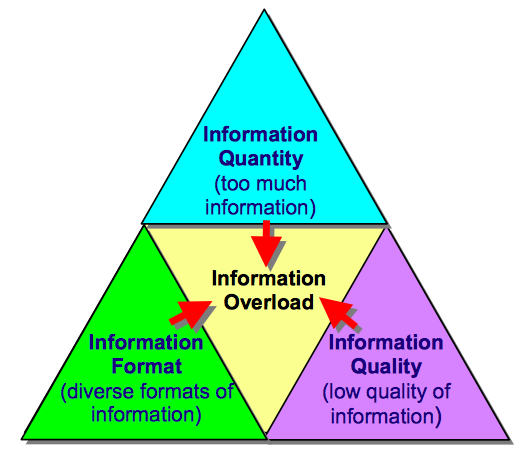
\includegraphics[width=.5\textwidth]{img/lit-survey/overload-model.png}
	\caption{Dimensions of information overload, as defined by \citet{TowardsAnOptimalResolutionToInformationOverload}.}
	\label{fig:dimensions}
\end{figure}

These factors correspond directly to the three points previously identified from the \citeauthor{anewmodelfornews} study. High information quantity leads to news fatigue, information format determines the level of possible story resolution, and information quality determines how much depth a reader can gain from the news they consume. The authors did not find a single solution which could address all three factors, but they did identify information quantity as the most significant contributor to overload.

\citet{GuestEditorsIntroductionInformationOverload} further decompose information quantity into spatial and temporal dimensions in the specific context of news articles. Spatial quantity refers to articles which are near-identical in terms of facts presented being published by different media outlets, and temporal quantity refers to articles on a single topic being published in quick succession over a short period of time. 

Intuitively, the terms spatial and temporal quality seem illogically named, as a set of articles with high spatial quantity would cover a smaller area of information space and vice versa. High spatial quantity will therefore be referred to as \textit{redundancy}, and high temporal quantity as \textit{fragmentation}, since a sudden burst of articles published on the same topic suggests a currently unfolding story being told in parts.

To adequately determine the contributory factors relating to news fatigue, all four dimensions of information overload should be considered, and will therefore be explored in more detail in the following sections.

\subsubsection{Information Quality}
In the context of factual data rather than news specifically, \citet{DataQualityInContext} defined information quality in terms of four components; intrinsic quality, accessibility quality, contextual quality and representational quality. If news can be rationalised to its core function as an interpretation of facts and other raw data such as images, then this same framework can be experimentally applied to news journalism in order to determine which factors could influence its quality.

Intrinsic quality is a measure of the accuracy, objectivity, believability and reputation of data. In the context of news, the first three factors would typically be true for all major news sources, and the reputation would be dependent on whether the article originated from a trusted source or not. Accessibility quality is less relevant to online news media, as it is concerned with data access and security. Contextual quality is the most relevant category in respect to news, concerning timeliness, amount of data, and value-added. In the news domain, this would mean an article's quality is dependent on its performance against a background of other articles; whether or not it contributes anything recent or previously unknown. Finally, representational quality is concerned with ease of understanding and interpretability, which are easily translatable concepts.

The implications of applying the Information Quality Framework \citep{DataQualityInContext} to news articles are that quality may be influenced by the reputation of the source, the timeliness of publication, value-added by the article (i.e. content which couldn't be derived from other sources) and the ease of understanding of the content.

\subsubsection{Information Format}
The domain of news articles is a more specific information space than that of documents in general, and by nature most news articles share some common formatting and structural elements such as headlines, timestamps, and relevant images. As a result of this, it is unlikely that any two articles from popular news providers would be diverse enough in content format to overshadow the information quantity problem.

\subsubsection{Fragmentation (Temporal Quantity)}

The rise of social media sites such as Twitter delivering news to consumers has lead to a high degree of news fragmentation, due to the constraints of the microblogging service's 140-character limit. 24-hour television news paved the way for new formats of real-time content delivery, and the ever-expanding network of online social media channels stepped up to deliver. 

It logically follows from the fragmented nature of real-time news journalism that temporal quality suffers; stories are published and updated intermittently over short periods of time, meaning there is more content for the consumer to piece together in order to understand a story. The fragmentation is somewhat mitigated by Twitter's use of hashtags to denote a Tweet's topics. Hashtags help readers form a coherent and picture of unfolding events from the incremental contributions of thousands of participating users \citep{BlogsTwitterAndBreakingNews}.

\citet{BreakingNewsDetectionAndTrackingInTwitter} developed a methodology to collect and group Tweets on breaking news topics, using hashtags for topic identification or \textit{story-finding}, and grouping similar messages together to form a single news story. Their algorithm for similarity is a function of the tf-idf \citep{TermWeightingApproachesInAutomaticTextRetrieval} of the two messages and the number of named entities they have in common.

\subsubsection{Redundancy (Spatial Quantity)}
It is in the nature of news that newsworthy stories get repeated across multiple sources. When consumers read news on a particular from more than once source, it is likely that they will read variations on the same facts in multiple articles.

Attempts such as \citep{InformationFusionInTheContextOfMultiDocumentSummarization} have been made to synthesise summaries of collections of similar online documents, a practice here termed \textit{information fusion}, with news articles from different sources being given as a specific use-case. However, the process of extracting common sentences between documents was in order to reformulate them into a single summary, rather than to determine the level of similarity between the documents.

A more relevant approach was presented by \cite{UtilizingPhraseSimilarityMeasures}, who used the \textit{title} and \textit{description} attributes of elements in RSS feeds as content descriptors to mitigate the overhead of processing entire documents for phrases. The content descriptors are then used to compute phrase \textit{n}-grams as a measure of similarity between any two documents. The similarities in this case were used to remove subsumed articles and cluster non-redundant similar ones, in order to streamline feed content for readers.

It should be noted that there is an overlap between the notion of spatial quantity and one of the four influencing factors in information quality; contextual quality. If a feed contains two articles which state the same number of identical facts, they therefore contribute to information overload on both the qualitative and quantitative fronts.

Viewing the dimensions of overload from a news domain perspective, it is clear that (consistent with the findings of \citet{TowardsAnOptimalResolutionToInformationOverload}) information quantity is the most relevant contributing factor in respect to fatigue, along factors influencing contextual quality such as value-added and timeliness. Any proposed solutions to the news overload problem should therefore address these factors first.

\subsection{Supporting Sensemaking}

Sensemaking is the basis for forming contextual knowledge; the process by which we incorporate new information into our existing cognitive frameworks, and how we go from reading something to understanding it \citep{FromInformationToKnowing}. In broader terms, \citeauthor{OrganizingAndTheProcessOfSensemaking} describe sensemaking as ``[being] about the question: What does an event mean? In the context of everyday life, when people confront something unintelligible and ask, `What's the story here?'{}'' \citep[p.85]{OrganizingAndTheProcessOfSensemaking} 

This definition relates directly to the news overload problem because one component of sensemaking is the contextual story resolution The \citet{anewmodelfornews} study identified news consumers are craving. It has also been observed that often readers are not interested in specific articles on a subject, and only the thematic content of the topic they belong to \citep{AnalysingUserAccessToAnOnlineNewspaper}. How then, do readers make sense of a collection of articles surrounding a particular topic?

When presented with a large document collection, \citet{BeingLiteratreWithLargeDocumentCollections} found all of their subjects began by clustering the contents into groups which formed a heuristic representation or mental model, used to provide an overview. However, current information infrastructure has been criticised for not supporting the cross-correlation between connected news articles \citep{GalaxyOfNews}.

Writing for the Columbia Journalism review in 2008, \citeauthor{overloadjournalismsbattle} outlined a suggestion for the new roles of journalism in the information era; ``By linking stories to one another and to background information and analysis, news organizations help news consumers find their way through a flood of information that without such mediation could be overwhelming and nearly meaningless''\citep[p.10]{overloadjournalismsbattle}. 

Similarly, \citet{FromInformationToKnowing} make the recommendation in the context of contemporary media consumption that news providers should adapt to an environment of news overload by adding facilities enabling readers to categorise, sort and search news collections. Additional findings of this study suggested that the contextual background provided by having more detailed coverage aids the sensemaking process, as it helps users form links between new information and their existing frameworks, but this presents an interesting conflict with the goal of reducing information overload when considering large collections of documents.

It is apparent that many recommendations have been made from within the field of journalism that at the point of delivery, news content should incorporate contextual links between related articles. This is important both from a sensemaking perspective to emphasise connections, and from an information overload perspective to help users find meaning in an inundated news landscape.

The news overload problem can now be reformulated with scope and detail: How can we display a collection of related news articles in such a way that users are not overwhelmed by unstructured content and are free to explore the underlying contextual pathways?

A simple starting point comes from a familiar idiom; a picture is worth a thousand words.

\section{An Overview of Information Visualisation}

Of course, a picture is not always worth a thousand words, particularly when the picture is unstructured and complex in its own right. However, a recognised and effective technique for bridging the gap between a set of data and a user's mental model and subsequent comprension of the data is information visualisation, or InfoVis. \citep{UnderstandingAndCharacterizingInsights, ThemeRiver}. This section provides a brief overview of a formative InfoVis taxonomy and uses the taxonomy to categorise appropriate visual models for newsfeed visualisation.

In his seminal paper on information visualisation, \citeauthor{TheEyesHaveIt} proposed a taxonomy for visualisations comprising seven data type abstractions, and seven tasks which are components of the visual information seeking mantra; ``Overview first, zoom and filter, then details-on-demand.'' \citep[p.1]{TheEyesHaveIt}

\citeauthor{TheEyesHaveIt}'s type abstractions are as follows:
\begin{description}[leftmargin=11em,style=nextline]
	\item [1-dimensional] Linear data, where each datum is a string of characters.
	\item[2-dimensional] Planar data, e.g. layout diagrams, or clustered document collections.
	\item[3-dimensional] Physical objects or models of real-world entities, e.g. computer aided designs or medical imaging data.
	\item[Multi-dimensional] Any data where items with n attributes can be represented in n-dimensional space, e.g. relational databases, or feature vectors for classification.
	\item[Temporal] Data following a timeline, which is a subset of 1-dimensional data but was deemed important enough to warrant its own category. E.g. Project management data, or multimedia content timelines.
	\item[Tree] Hierarchical data where each datum has exactly one parent and zero or many children, e.g. document or directory structures.
	\item[Network] Related data, where each datum can have an arbitrary number of links to other data.
\end{description}

Because of the non-spatial nature of textual data, any visualisation of such data must involve some form of content abstraction and translation into a physical space \citep{VisualizingTheNonVisual}. These translations can result in data of arbitrary dimensionality, so a text corpus could fall into the 1-dimensional or multi-dimensional categories. News articles as a specific subset of textual data have certain metadata associated with them including dates, meaning they also fit the temporal type abstraction. In addition to this, if contextual links are considered part of the structure of the data, articles can be modelled as a network of connected nodes.

This ambiguity is not a failure of the taxonomy; \citeauthor{TheEyesHaveIt} stresses that composite categories are equally valid. However, the implications of this are that the most appropriate visualisation for a news corpus may itself be a composite of visualisations for any of its type abstractions, leaving an unfeasible number of possibilities to consider. 

To reduce the scope of suitable visualisations, we return to the original problem of information overload. This time however, the aim is to minimise the overload from interpreting the model, rather than the overload from interpreting the data. Complex visualisations which require a considerable amount of effort to understand in their own right should be avoided where possible when reducing overload is the goal.

\subsection{InfoVis for Sensemaking}

In addition to the insight that visualisation may be able to provide, there is evidence that visual metaphors better support the learning process and are more easily remembered than isomorphic text representations alone \citep{KnowledgeMapsAsScaffolds, ImageBasedConceptMapping}.

\citet{UnderstandingAndCharacterizingInsights} identified four overlapping InfoVis processes which describe how insight can be gained after sensemaking; \textit{Provide Overview}, \textit{Adjust}, \textit{Detect Pattern}, and \textit{Match Mental Model}. These four processes can be roughly mapped to \citeauthor{TheEyesHaveIt}'s high-level tasks, which are as follows:

\begin{description}[leftmargin=11em,style=nextline]
	\item [Overview] Gain a birds-eye view of the entire collection, with the option to change the scale of the view by zooming or using fisheye magnification techniques.
	\item[Zoom] Gain a more detailed view of a portion of data or single datum while preserving the original sense of context.
	\item[Filter] Nondestructively remove uninteresting data points or groups from the view.
	\item[Details-on-Demand] Gain additional insight into one or more data points by selecting particular elements.
	\item[Relate] View and explore relationships between elements.
	\item[History] If necessary, undo previous actions to return to the a view of the data.
	\item[Extract] Export selected data, preserving the format, for uses such as ``sending by email, printing, graphing, or insertion into a statistical or presentation package'' \citep[p.5]{TheEyesHaveIt}.
\end{description}

The \textit{Provide Overview} process allows a reader to recognise what they know and what they don't know from the information they are processing. The corresponding task in \citep{TheEyesHaveIt} is \textit{Overview}.

\textit{Adjust} allows them to change the level of abstraction or field of selection of that information. This corresponds to \textit{Zoom} and \textit{Filter} in \citeauthor{TheEyesHaveIt}'s task model.

The \textit{Detect Pattern} procedure is where structure and trends are found (whether expected or otherwise). Coupled with \textit{Match Mental Model}, where the links are formed between the new data and the users' existing cognitive frameworks, this corresponds to \textit{Relate}.

At this point, \citeauthor{TheEyesHaveIt}'s taxonomy diverges from the processes of \citep{UnderstandingAndCharacterizingInsights}, as \citeauthor{UnderstandingAndCharacterizingInsights} are concerned with the cognition enabled by visualisation, whereas  \citeauthor{TheEyesHaveIt} additionally considers other use cases for visualisations, such as querying and sharing.

From these two models, it is apparent that certain views and functions are crucial for tools which use visualisation to support the sensemaking process; an high-level overview visualisation which emphasises links between data, the ability to adjust scope to show more or less detail, and the ability to filter information of specific interest within the dataset.

\subsection{Visual Metaphors}

\citeauthor{AComparisonBetweenConceptMaps} defines visual metaphors as ``a graphic structure that uses the shape and elements of a familiar natural or man-made artefact or of an easily recognizable activity or story to organize content meaningfully and use the associations with the metaphor to convey additional meaning about the content.'' \citep[p.203]{AComparisonBetweenConceptMaps} This definition highlights the main advantage to using visual metaphors; users are intuitively familiar with how they present and structure information.

The use of preexisting visual metaphors--specifically those with which a large number of people will already be familiar--has been shown to support readers' comprehension, as it requires both significant time and effort for a reader to interpret visual metaphors which are new to them \citep{PreconceptionsVisualMetaphors}.

In a previous paper, \citeauthor{VisuelleKommunikation} also describes six advantages of visual metaphors specifically for the transfer of knowledge: ``(1) to motivate people; (2) to present new perspectives; (3) to increase remembrance; (4) to support the process of learning; (5) to focus the attention of the viewer and (6) to structure and coordinate communication.'' \citep[p.2, citing \citep{VisuelleKommunikation}]{LearningFromArchitects}. These are all desirable attributes, but motivation and support in the learning process are particularly relevant in addressing news fatigue.

Examples of visual metaphors commonly used to represent collections of data include calendars, bookshelves, timelines, maps and other schematics. Metaphors based on physical objects do not have to be visually skeuomorphic to be effective, but to avoid misinterpretation, there should be a match between the underlying structure of the metaphor and the underlying structure of the data. Two common and highly structured visual metaphors will be explored in the following sections in the context of potential for news representation; timelines and schematic maps.

\subsubsection{Timeline Visualisations}

Chronological ordering is an important characteristic of news articles and should be preserved in any visualisation of news data as it provides a natural ordering \citep{StructuredSummarizationForNewsEvents}. Perhaps the simplest visual metaphor for a collection of dated documents is the timeline.

\cite{SchemaLine} explore the role of timelines in the sensemaking process,  emphasising that the interactions supported by such visualisations should be as intuitive as possible in order to not disrupt users' trains of thought, and should be tightly coupled with other elements of the sensemaking process so temporal connections are not viewed solely in isolation.

Criticisms of previous timeline visualisations made by the authors are that linear layouts  are often too simple for the data they represent, and that a lack of automatic layout generation results in additional manual work for the user.

The colouring technique used to distinguish sets of related events within a single timeline is a flexible extension to \citep{TimeSets}, where the authors coloured events belonging to multiple sets with a gradient composed of the colours of both sets. However, the gradient approach presented in \citep{SchemaLine} does not scale to events belonging to more than two sets, since the colour grouping restricts the number of possible intersections of each set. From a news storyline perspective, this would place an upper limit of two on the number of possible topics a story could belong to, which is a low constraint for all but the highest level topics.

\citet{ExploringLongRunningNewsStoriesUsingWikipedia} designed a prototype for generating annotated timelines based on the Wikipedia entries long-running news stories. The use of Wikipedia rather than newsfeeds meant their document retrieval model was heavily dependent on Wikipedia's structure, but it also afforded a huge wealth of contextual information that made such detailed annotations possible. Not all stories are long running however, so while this would be useful as a retrospective tool it would be impossible to generate timelines in the same way for news articles which did not already belong to a long-running chain of events.

\begin{figure}[h]
\centering
\begin{minipage}{.45\textwidth}
  \centering
  \hspace{-1cm}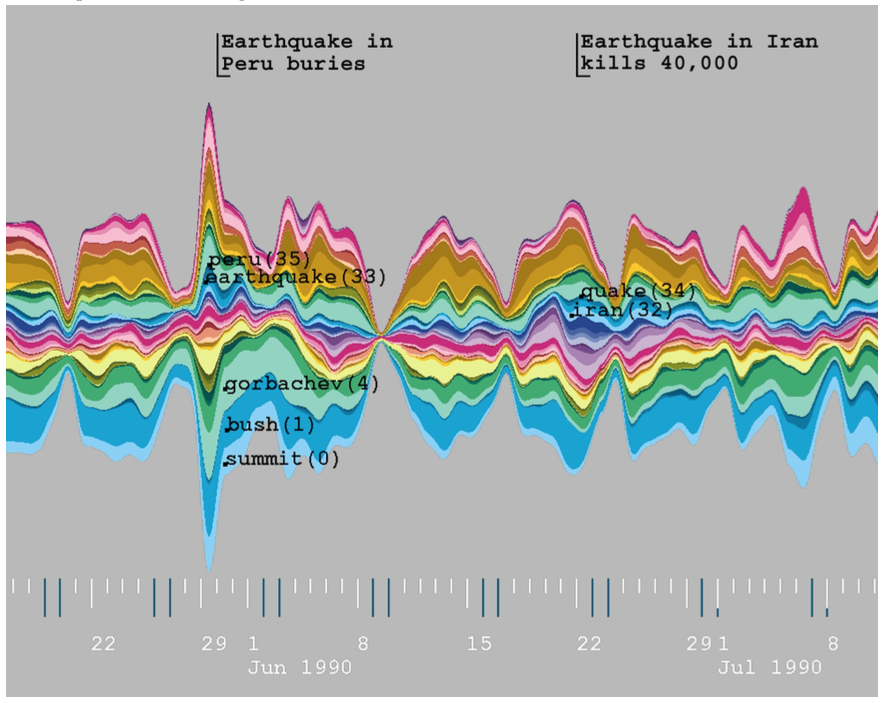
\includegraphics[width=.9\linewidth]{img/lit-survey/histogram1.png}
  \end{minipage}%
\begin{minipage}{.65\textwidth}
  \centering
  \hspace{-1.5cm}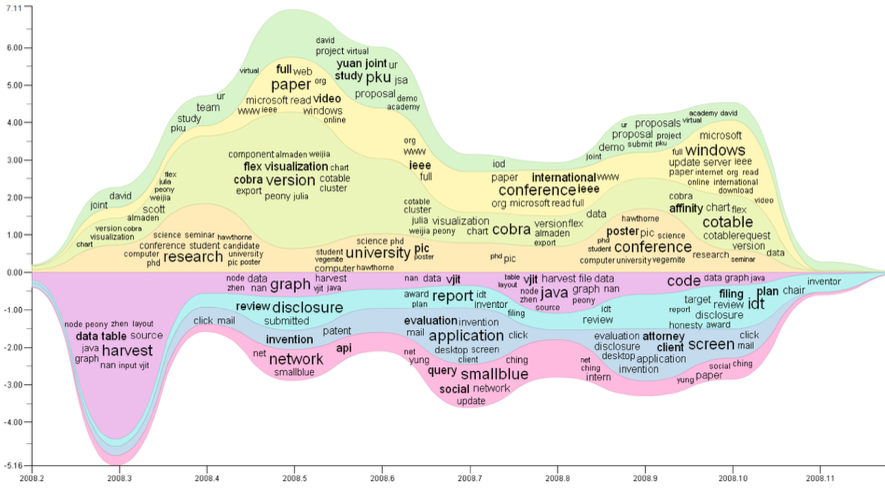
\includegraphics[width=.9\linewidth]{img/lit-survey/histogram2.png}
\end{minipage}
\caption{Similar visualisations from ThemeRiver \citep{ThemeRiver} (left) and TIARA \citep{InteractiveTopicBasedVisualTextSummarizationAndAnalysis} (right).}
  \label{fig:themeriver-tiara}
\end{figure}

Both ESTHETE \citep{ESTHETE} and nReader \citep{Nreader} present timeline-centric views for collections of news articles based on underlying graphs of relationships between the articles. However, in both cases, the graph structure was not part of the final visualisation, so connections between entities were displayed in purely textual forms. In contrast, ThemeRiver \citep{ThemeRiver} introduces a novel view on topic frequency along the time axis to show thematic change over time within a collection of documents, similar to a smoothed histogram. This view, while useful for large document collections which span weeks or months, would be less suited to displaying emerging news trends over shorter periods.

TIARA \citep{InteractiveTopicBasedVisualTextSummarizationAndAnalysis} whose authors cite ThemeRiver as an influencing design (see figure \ref{fig:themeriver-tiara}), displays a similar shaped graphical output but performs more detailed textual analysis, and displays related keywords in the output. Both visualisations support simple zooming and panning, but suffer from the same limitations on visualising topic connectivity as \citep{TimeSets}.

Taking into consideration both the critiques of  oversimplification identified in \citep{SchemaLine} and the physical limitations highlighted in \citep{TimeSets, ThemeRiver}, it is clear that timelines may not be the most appropriate visual metaphor for news visualisation, especially not for highly connected events and topics. However, for more linear storylines which span fewer categories or topics, a visualisation such as \citep{SchemaLine} could be used, for example as part of \citeauthor{TheEyesHaveIt}'s \textit{Zoom and Filter} task where the dataset is pruned.

\subsubsection{Topological and Schematic Map Visualisations}

The use of cartographic representations for abstract objects and the relationships between them is such a common and natural metaphor that it is often unnoticed in digital contexts. Maps take advantage of humans' natural ability to perceive and organise in a spatial context, and [the fact that we live in a spatial world] ``leads naturally to metaphors that provide cues for orientation and navigation'' \citep[p.2]{InformationCartographyUsingGIS}.

Topological maps\footnote{Not to be confused with \textit{topographic} maps, which represent relief and other geographic features of physical regions at a large scale and in fine detail.} are a specific class of map which abstract away detail so that only significant features within desired subsets of the mapped dataset remain; from a news overload perspective, this is a highly desirable property. These maps are often used to visualise networks and are represented as schematics, where elements on the map are transformed into abstract visual representations for ease of understanding. Today, the most recognisable examples of topological maps are transit maps. Divorced from the strictness of geographical accuracy and scale, emphasis is instead placed on the usability of the map for planning and the understanding of relative positioning which the maps enable \citep{TheInfluenceOfMapDesignOnRouteChoice}.

\begin{figure}[hp!]
	\centering
	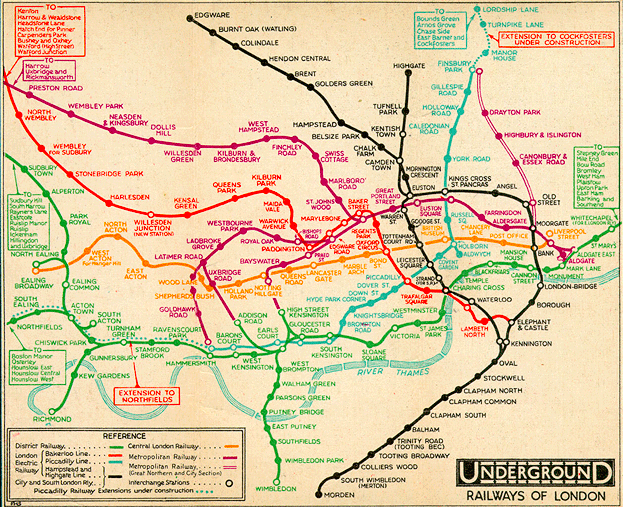
\includegraphics[width=.8\textwidth]{img/lit-survey/1930-pre-beck.png}
	\caption{1930 London Underground map, designed by F. Stingemore \citep{Tube150}.}
	\label{fig:pre-beck}
\end{figure}

\begin{figure}[hp!]
	\centering
	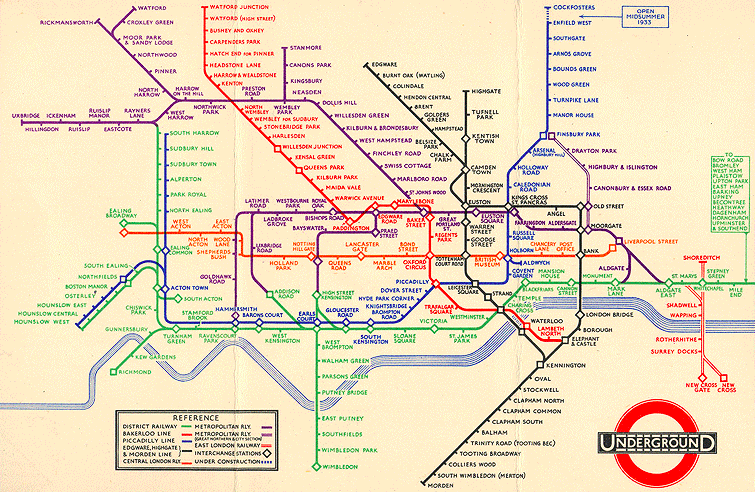
\includegraphics[width=.8\textwidth]{img/lit-survey/1933-beck.png}
	\caption{1933 London Underground Map, designed by H. Beck \citep{Tube150}.}
	\label{fig:beck}
\end{figure}

Figures \ref{fig:pre-beck} and \ref{fig:beck} show the geographically accurate 1930 London Underground map designed by Frederick Stingemore, and the iconic 1933 redesign by Henry Beck, which was based on the concept of an electrical circuit diagram \citep{HarryBeck}. While Beck's simplification of the structure of the map was seen as radical and even controversial at the time, the hallmarks of his design are now recognisable not just in other schematic maps, but in posters, infographics and diagrams across various domains.

In terms of usability, simple timeline visualisations can provide the chronological ordering which is intrinsic within collections of news articles. However, schematic maps may be able to represent complex relationships between topics in a structure which is linear but has an additional dimension, to prevent linearity becoming a design or usability constraint.

\section{Metro Maps for Information Cartography}
Significant work in the area of information cartography has been undertaken by Shahaf et al. \citep{ConnectingTheDots, GeneratingInformationMaps, MetroMapsOfScience, InformationCartographyPre}, in the domains of both news and science through the visualisation of article and journal data on metro maps.

\cite{GeneratingInformationMaps} chose the metaphor as a base for their visualisation to address the fact that previous timeline-based summarisation systems could only represent simple linear stories; ``In contrast, complex stories display a very non-linear structure: stories split into branches, side stories, dead ends, and intertwining narratives.'' \citep[p.1]{InformationCartographyPre}

\begin{figure}[htbp!]
	\centering
	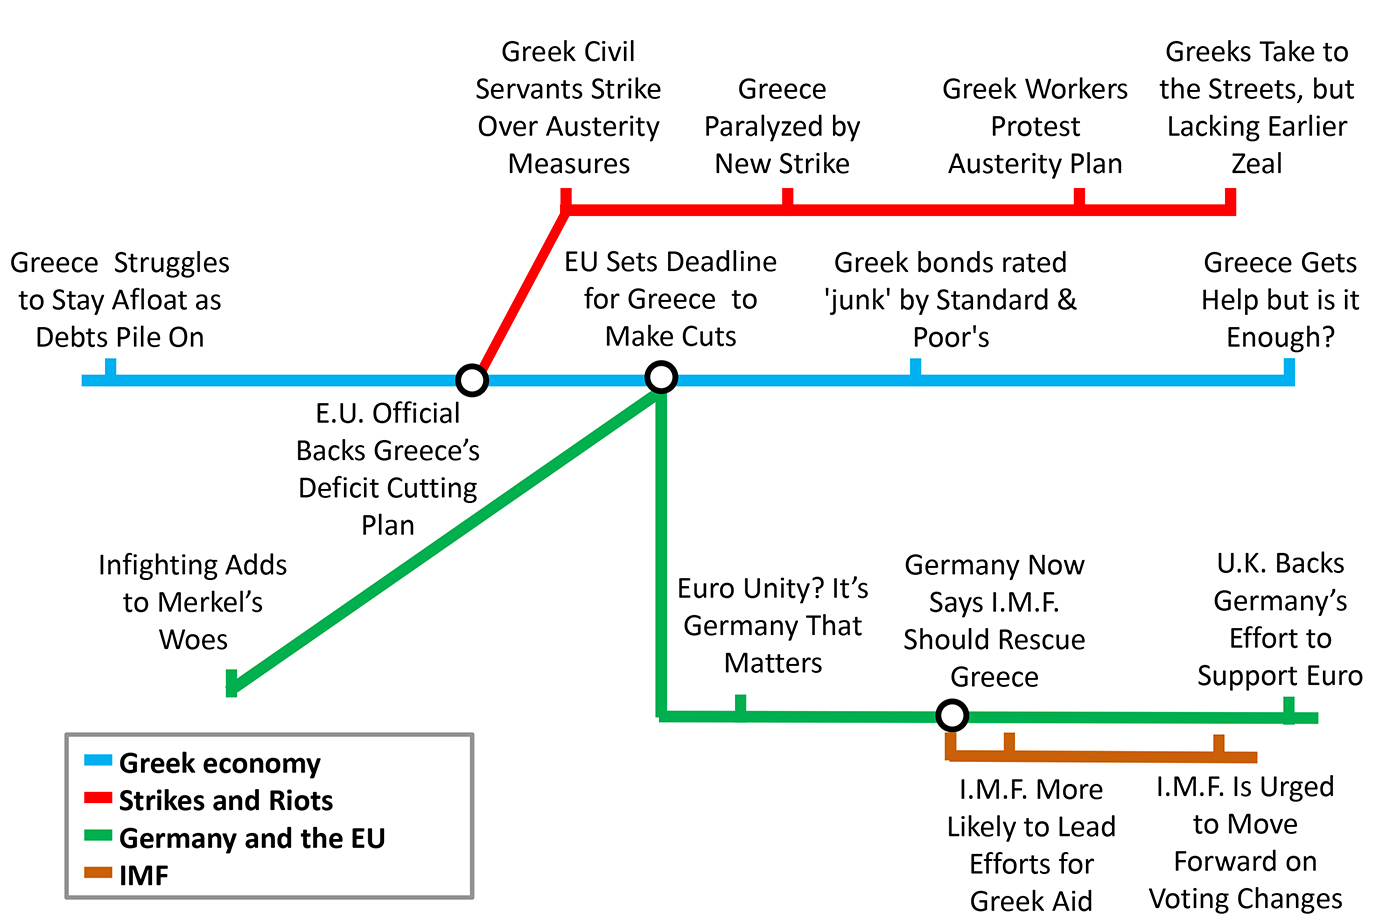
\includegraphics[width=.8\textwidth]{img/lit-survey/greece-metromap.jpg}
	\caption{A metro map \citep{GeneratingInformationMaps} covering the Greek Debt Crisis.}
	\label{fig:greecemetro}
\end{figure}

Even in a scientific context, this was not the first time the abstract visualisation potential of the metro map had been noted; ``The usefulness of the metro map as a metaphor is somewhat limited to simple examples by the time required to manually produce these maps. As such they are generally only useful for applications that do not change frequently. This limitation could be removed by quality methods for the automatic drawing of metro maps from abstract data.'' \citep[p.54]{AutomaticMetroMapLayoutThesis}

In this section, the formalisation of the metro map metaphor, its associated characteristics, and its limitations will be discussed.

\begin{definition}{Metro Map \citep{GeneratingInformationMaps}:}
A metro map $\mathcal{M}$ is a pair $(G, \Pi)$, where $G=(V, E)$ is a directed graph and $\Pi$ is a set of paths, or \textit{metro lines} in $G$. Each $e \in E$ must belong to at least one metro line.
\label{def:mm}
\end{definition}

A previously published method \citep{ConnectingTheDots} for linking together chains of articles  was discussed, and an objective function was created to formalise the characteristics of a `good' metro map. The function defined was a composite based on three important characteristics, all of which are broadly applicable to the visualisation of any similar corpora; coherence, coverage, and connectivity.

\subsection{Coherence}
Let $\mathcal{D}$ be a set of articles, and $\mathcal{W}$ be a set of words or phrases, such that each article is a subset of $\mathcal{W}$. A \textit{coherent} chain of articles through $\mathcal{D}$ is one where transitions between documents are smoothed by common overlapping keywords from $\mathcal{W}$, creating a better narrative flow \citep{ConnectingTheDots} as depicted in Figure \ref{fig:coverage}.

\begin{figure}[htbp!]
	\centering
	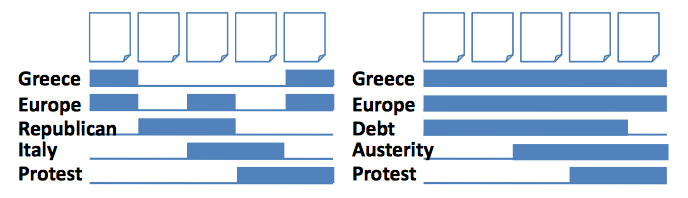
\includegraphics[width=.7\textwidth]{img/lit-survey/coverage.png} \par
	 A bar corresponds to the presence of a word in the article above it.\\The titles of the articles which made up the two chains were as follows:\\[0.2cm]\footnotesize{
	 \begin{tabular}{|l|l|}
	 	\hline 
	 	Chain A (left) & Chain B (right) \\
	 	\hline
	 	Europe weighs possibility of debt default in Greece & Europe weighs possibility of debt default in Greece \\
	 	Why Republicans don't fear a debt default & Europe commits to action on Greek debt \\
	 	Italy; The Pope's leaning toward Republican ideas & Europe union moves towards a bailout of Greece \\
	 	Italian-American groups protest `Sopranos' & Greece set to release austerity plan \\
	 	Greek workers protest austerity plan & Greek workers protest austerity plan \\
	 	\hline
	 \end{tabular}\vspace{0.2cm}}
	 \caption{An incoherent chain with jittery transitions between topics (Chain A, left) alongside a more coherent chain of articles (Chain B, right). \citep{GeneratingInformationMaps}}
	\label{fig:coverage}
\end{figure}

Coherence, intuitively, seems to be closely linked to idea of story resolution detailed in Section \ref{sec:information-overload}. This presents a question which could later be explored further; does forming coherent chains of articles provide the story resolution that participants in the Associated Press study were so desperately seeking from current events journalism?
	
\subsection{Coverage}
As in the previous section, let $\mathcal{D}$ be a set of articles, and $\mathcal{W}$ be a set of words or phrases of which the articles are composed. The coverage function for a word in a given document $d_i \in \mathcal{D}$ specified in Equation \ref{eqn:doc-coverage} can be quantified using any measure of how well $d_i$ covers $w$, for example tf-idf$(w, d_i, \mathcal{D})$ (See Equation \ref{eqn:tfidf}) \citep{GeneratingInformationMaps}.
\begin{equation}
	cover_{d_i}(w) : \mathcal{W} \rightarrow [0,1]
	\label{eqn:doc-coverage}
\end{equation}
Extending the notion of coverage to maps--which can be abstracted to sets of documents--introduces the idea of \textit{diversity}. If a map already contains documents which for a sufficient coverage for some word $w$, then there is nothing to be gained by adding another document to $\mathcal{D}$ which has high coverage of $w$ alone. This relates back to the principles of spatial and information quality discussed in Section \ref{sec:information-overload}, especially the importance of value-added by every individual document in a collection. In this case, maps which cover a maximal number of $w \in \mathcal{W}$ should be preferential. A simple additive definition for map coverage such as Equation \ref{eqn:additive-coverage} \citep{GeneratingInformationMaps} would not reward this kind of diversity;
\begin{equation}
	\label{eqn:additive-coverage}
	cover_\mathcal{M}(w) = \sum_{d_i\in docs(\mathcal{M})}cover_{d_i}(w)
\end{equation}
Therefore, an alternative definition for map coverage was chosen, which will not increase significantly if another document which covers an already covered feature is added to $\mathcal{D}$ (Equation \ref{eqn:multiplicative-coverage} \citep{GeneratingInformationMaps}).
\begin{equation}
	\label{eqn:multiplicative-coverage}
	cover_\mathcal{M}(w) = 1 - \prod_{d_i\in docs(\mathcal{M})}(1-cover_{d_i}(w))
\end{equation}
Finally, the definition of map coverage is extended to the coverage of the corpus $\mathcal{D}$, rather than just single features. If each feature is weighted according to frequency, then for each $w \in \mathcal{W}$ we have some $\lambda_w$. The coverage of a corpus $\mathcal{D}$ by a metro map $\mathcal{M}$ can then be defined as in Equation \ref{eqn:map-coverage} \citep{GeneratingInformationMaps}.
\begin{equation}
	\label{eqn:map-coverage}
	Cover(\mathcal{M}, \mathcal{D}) = \sum_{w \in \mathcal{W}}\lambda_w cover_\mathcal{M}(w)
\end{equation}

\subsection{Connectivity}
The final property is the most simply defined; the connectivity of a metro map is the number of paths in $\Pi$ which intersect \citep{GeneratingInformationMaps}.
\begin{equation}
	Connectivity(\mathcal{M}) = \sum_{i<j}\mathbbm{1}(p_i \cap p_j \neq\emptyset)
\end{equation}

\subsection{Limitations of \cite{GeneratingInformationMaps, InformationCartographyPre}}

\subsubsection{Corpus}
Perhaps the biggest limitation of the system developed in \citep{GeneratingInformationMaps, InformationCartographyPre} is the nature of the corpus $\mathcal{D}$; it is a fixed dataset, meaning users can only query it for certain past events with no way of specifying a different corpus themselves.

From a historical reference perspective the output generated based on certain queries is interesting when compared to the output an expert would select as important to the narrative, but it is not possible to use the system as a replacement to a newsfeed aggregator.

\subsubsection{Graph Layout Aesthetic Principles}

From a usability perspective, a second limitation of the work of \citeauthor{GeneratingInformationMaps} is the lack of focus given to the desirable aesthetic properties of transit maps.

A formative empirical study \citep{TheBasisForGraphDrawingAlgorithms} on how graph layout affects usability identified a collection of five measurable aesthetic principles from previous research, which aid human understanding when reading graphs:
\begin{itemize}[noitemsep]
	\item Minimise the number of line bends \citep{MinimiseBends};
	\item Minimise the number of edge crossings \citep{MinimiseEdgeCrossings};
	\item Preserve any underlying symmetry in the structure of the graph \citep{PreserveSymmetry};
	\item Draw orthogonally where possible \citep{MinimiseBends};
	\item Maximise the minimum angle between incident edges for each node \citep{IncidentEdges}.
\end{itemize}
These criteria, when numerically calculated and weighted relative to one another, allow the aesthetic quality of any graph to be evaluated. This is particularly useful for graphs generated by automatic layout algorithms, which aren't as much a product of human design intuition as their manually designed counterparts.

The origins of the principles above predate much of the early InfoVis research because several of them \citep{MinimiseBends, MinimiseEdgeCrossings} were formalised as guidelines for the design of electronic circuits.

In a later study, \citeauthor{WhichAesthetic} evaluated information-finding task performance with a set of graphs which varied the above principles, to establish which the most and least significant aesthetics were for graph usability. The results of the study were that maximising incident edge angles and orthogonality did not lead to better performance, preserving symmetry and minimising line bends were somewhat important, and minimising edge crossings was the most significant influencing factor for performance \citep{WhichAesthetic}. 
 
Metro maps, however--particularly those representing non-physical data such as in the previous section--do not share all the structural principles of the wider set of directed graphs. Consequentially, \citeauthor{AutomaticMetroMapLayout} developed a set of criteria for metro maps specifically, including criteria for the labelling of stations. The criteria are as follows \citep{AutomaticMetroMapLayout}:

\begin{itemize}
	\item \textbf{Angular Resolution Criterion:} Maximise the angle between incident edges at each node. This criterion is also the fifth principle in \citep{TheBasisForGraphDrawingAlgorithms}. 
	\item \textbf{Edge Length Criterion:} All edges on the map should be approximately equal.
	\item \textbf{Balanced Edge Length Criterion:} The length of edges incident to a given node should be approximately equal.
	\item \textbf{Edge Crossings Criterion:} Crossings should be minimised. This criterion is also the second principle in \citep{TheBasisForGraphDrawingAlgorithms}, also identified as the most important.
	\item \textbf{Line Straightness Criterion:} Edges on the same metro line should be collinear, i.e. they should form a 180$^{\circ}$ line through every station that the line passes through. This criterion relates closely to the first principle in \citep{TheBasisForGraphDrawingAlgorithms}.
	\item \textbf{Octilinearity Criterion:} Edges should be drawn at multiples of 45$^{\circ}$. This criterion is an extension to the fourth principle in \citep{TheBasisForGraphDrawingAlgorithms}, as orthogonality is here analogous to rectilinearity.
\end{itemize}

Evaluating Figure \ref{fig:greecemetro} according to the list above, we observe that despite only containing 16 stations, the map unnecessarily violates five  of \citeauthor{AutomaticMetroMapLayout}'s six criteria--all except edge crossings.

Therefore, to improve the usability of the metro maps drawn in \citep{ConnectingTheDots, GeneratingInformationMaps, MetroMapsOfScience, InformationCartographyPre}, it would be advisable to attempt to satisfy more of the aesthetic principles for graphs and metro maps described in \citep{TheBasisForGraphDrawingAlgorithms, AutomaticMetroMapLayout}.


\section{Towards Newsfeed Visualisation}

The fact that news articles form a fairly narrow class of document is an advantage from a visualisation design perspective, due to the common elements they share. Articles published by commercial news producers typically contain:
\begin{itemize}[noitemsep]
	\item A headline;
	\item A description, or \textit{subhead};
	\item A publish date;
	\item One or more categories to which the article belongs.
\end{itemize}
These attributes are useful for visualisation, since creating a spatial representation from text requires documents to be represented as vectors in high-dimensional feature space \citep{VisualizingTheNonVisual}, and the presence of existing attributes makes articles more inherently comparable than their unstructured contents would be.

There is also a well-known existing standard for publishing links to articles with their metadata for use by other applications; RSS.

\subsection{Content Retrieval}
The de-facto web format for feed publishing is RSS (Rich Site Summary, or Really Simple Syndication.) The rise of the internet as a news platform has lead to many readers finding the most efficient method of reading news articles is to subscribe to various topic-specific newsfeeds and read what is automatically collated by their computers \citep{Nreader}.

Although RSS--which is a subset of XML--is standardised\footnote{\url{http://cyber.harvard.edu/rss/rss.html}}, the practice of feed categorisation is not, meaning the granularity of topics which can be subscribed to is dependent on the publisher. This issue was addressed by \citet{PersonalNewsRss}, with the design of a system which could essentially split or join existing RSS feeds to synthesise new ones based on user-specified keywords and queries.

Despite its shortcomings, RSS remains the most universal option for accessing feed content from a wide variety of news producers 
\citep{MiningAndVisualisingInformationFromRSSFeeds}.

\subsection{Keyword Extraction}

Extracting relevant keywords from documents is not a new domain of research. Various methods have been presented, the most well-known being the intuitively logical tf-idf (term frequency, inverse document frequency) \citep{TermWeightingApproachesInAutomaticTextRetrieval} which ranks the significance of a term \textit{t} in a document \textit{d} which belongs to a corpus \textit{C} as follows:

\begin{equation}
	\text{tf-idf}(t) = \frac{Occurrences(t, d)}{WordCount(d)} \times log_e\bigg(\frac{|C|}{|\{c \in C \mid t \in c\}|}\bigg)
\label{eqn:tfidf}
\end{equation}

tf-idf will extract the most unique keywords from a document within a corpus, because it penalises words which are common to many documents. However, in the context of a corpus of news articles, this uniqueness can lead to significant topic keywords being ignored because they appear with such frequency. 

\citet{TopicExtractionfromnewsArchiveUsingTFPDFAlgorithm} found that for news archive keyword extraction, a better alternative to tf-idf is tf-pdf (term frequency, proportional document frequency) as it is not biased against frequently repeated keywords.

Using tf-pdf, articles are modelled as belonging to one of a finite number of sources or \textit{channels} within a corpus. The weighting of a term from an article within a channel is in this case linearly proportional to its frequency in the channel and exponentially proportional to the number documents in the channel where it occurs. A term's total weighting is the sum of its weightings across all channels, as can be seen in Equation \ref{eqn:tfpdf} \citep{TopicExtractionfromnewsArchiveUsingTFPDFAlgorithm}, where:
\begin{itemize}[noitemsep]
	\item $D$ = The number of channels in the corpus;
	\item $K_c$ = The total number of terms in channel $c$;
	\item $F_{tc}$ = Frequency of term $t$ in channel $c$;
	\item $n_{tc}$ = The number of articles in channel $c$ where term $t$ occurs;
	\item $N_c$ = The total number of articles in channel $c$.
\end{itemize}
\begin{equation}
	\label{eqn:tfpdf}
	\text{tf-pdf}(t, D, K) = \sum_{c=1}^{c=D}\frac{F_{tc}}{\sqrt{\;\sum\limits_{k=1}^{k={K_c}}{F_{kc}}^2}}\times\text{exp}{\bigg(\frac{n_{tc}}{Nc}\bigg)}
\end{equation}

The reliance of both tf-idf and tf-pdf on a fixed background corpus results in a need to recompute the function for every document if any are added to or removed from the collection. This is impractical for large collections, and even in the case of large fixed collections it does not scale well, which has resulted in the development of other methods.

An approach derived from energy levels in quantum systems was proposed in \cite{LevelStatisticsOfWords}, where keywords were extracted based on their spatial distributions within a single text. The theory behind the approach is that typically, keywords occurrences are distributed in significant frequency clusters throughout a document, whereas non-relevant words are distributed with uniform frequency (see Figure \ref{fig:ols-spectra}).

\begin{figure}[htbp!]
	\centering
	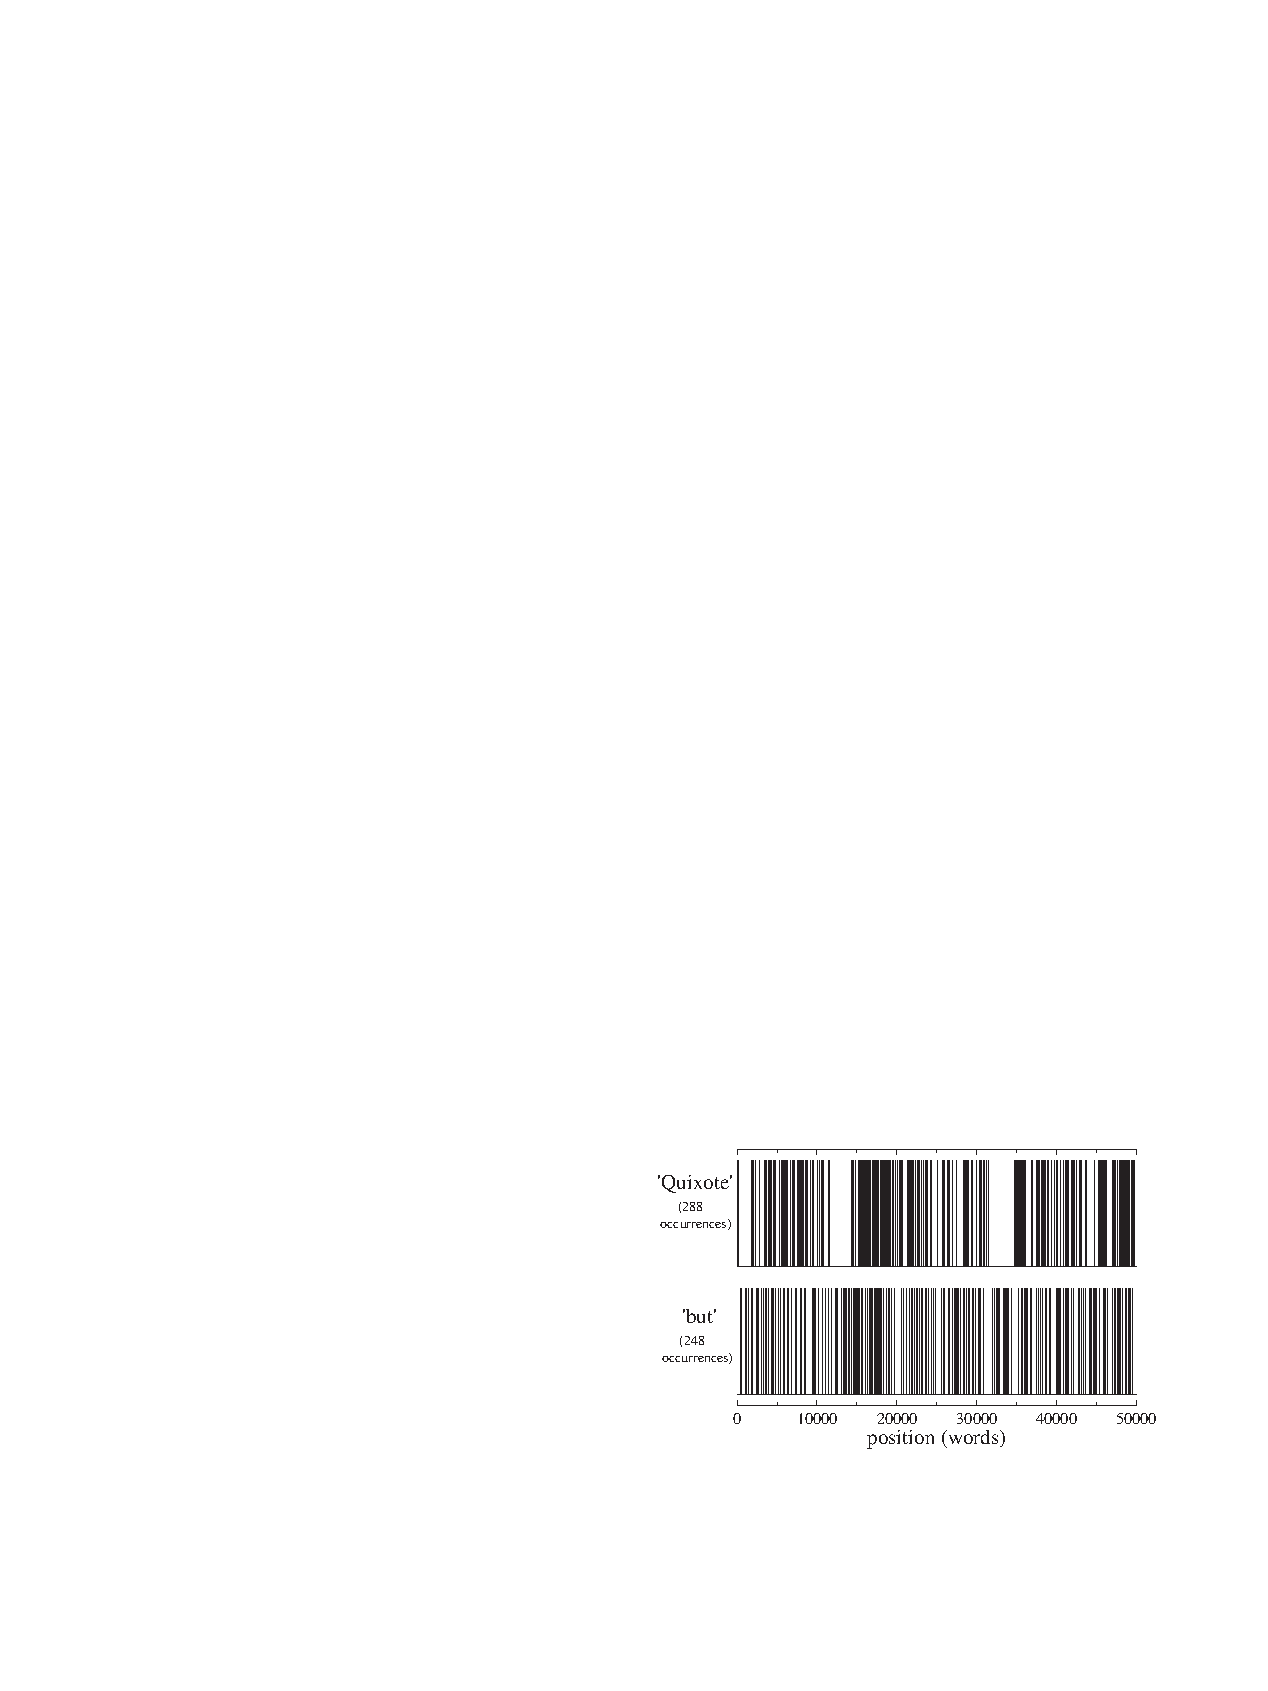
\includegraphics[width=.6\textwidth]{img/lit-survey/ols-keyword-spectra.pdf}
	\caption{Frequency spectra for `Quixote' and `but' in the first 50,000 words of \textit{Don Quixote}. \citep{LevelStatisticsOfWords}}
	\label{fig:ols-spectra}
\end{figure}

This technique allows relevant keywords to be distinguished from non-relevant common words with similar total frequencies without the use of a background corpus for comparison.

Several important observations have been made regarding keyword extraction for news articles specifically. Firstly, that important phrases in text are likely to be references to people, places and other named entities \citep{NewsStand}. Libraries such as the Stanford Named Entity Recognizer (NER) \citep{NestedNamedEntityRecognition} exist to extract these from text. 

Secondly, that while 30\% of an article's keywords are inferred and cannot be found within the text without intelligent input, 60\% are present in the article's title and first few sentences \citep{IdentifyingTopicsByPosition}, since important facts are generally stated as part of an article's \textit{above the fold} content.

\section{Evaluation Methods}
\citet{GeneratingInformationMaps} evaluated their system both for accuracy and with a user study, though as previously discussed they did not evaluate the aesthetic properties of the generated maps. The accuracy evaluation tested whether the system included the most `important' (as decided by experts) documents in the map. 

The user study focused on the strength of the results returned by specific queries, where output was transformed into a structureless list in order for the study to be double-blind against the other methods. The evaluation was performed between-subjects, so background knowledge had to be controlled for. Output was compared with that from Google News and a TDT (Topic Detection and Tracking) method presented in \citep{SemanticLanguageModelsForTDT}. 

This approach to evaluation is less relevant to my proposed system, since it was actually evaluating the performance of the system in selecting documents based on a query, rather than visualising the documents on a map. In contrast, a visualisation and its usability is precisely the aspect of my process which I would need to evaluate.

%\citet{EvaluatingInformationVisualisations} found that the evaluation of measures of usability such as task completion time and effectiveness can only be accurately conducted as part of a summative formal experiment. This is because formative tests such as think-aloud experiments require users to alter their behaviour and leads to slower actions \citep{VerbalReportsAsData}.

The evaluation of TIARA \citep{InteractiveTopicBasedVisualTextSummarizationAndAnalysis} was a more relevant method than the Metro Map evaluation as it was conducted against a baseline system which did not share any of its advanced features, although it was tailored for the same task; email analysis. A series of questions were asked of participants, who used either TIARA or the baseline system to answer. The response time and accuracy of the participants was recorded, as well as their levels of satisfaction after completing the task. This evaluation used between-subjects designs and therefore required the use of a different dataset for each task, as the nature of the sensemaking means any repetition of the evaluation task on the same data would see participants' performance improve significantly due to recall alone.

\section{Summary}

To recap, this review began with an exploration of the problem of news overload using the findings of The \cite{anewmodelfornews}, a field study conducted into the news consumption habits of young people. The findings of the study were then discussed, firstly in the context of four dimensions of information overload \citep{TowardsAnOptimalResolutionToInformationOverload, GuestEditorsIntroductionInformationOverload} and secondly in terms of how they relate to sensemaking; the cognitive process this project aims to support.

Information visualisation was identified as one common approach to both support sensemaking and reduce information overload, so various methods for visualising text-based documents and news articles specifically were presented and compared \citep{ESTHETE, ThemeRiver, InteractiveTopicBasedVisualTextSummarizationAndAnalysis, ExploringLongRunningNewsStoriesUsingWikipedia, Nreader} as well as a more in-depth exploration of visual metaphors, in particular timeline, and schematic map visualisations. This section also featured the introduction of the metro map in its original context, before moving on to its use as a metaphor for visualisation in various domains.

Centrally, the work of Shahaf et al. \citep{ConnectingTheDots, GeneratingInformationMaps, MetroMapsOfScience, InformationCartographyPre} which is particularly relevant to the aims and objectives of this project was discussed in detail, with an explanation of key metrics (\textit{coherence}, \textit{coverage} and \textit{complexity}) defined in \citep{GeneratingInformationMaps} which are applicable to all graph-based representations of document collections. My main critiques of this body of work were the fixed background corpus and the physical layouts of the drawn maps when evaluated against the criteria defined in \citep{TheBasisForGraphDrawingAlgorithms, AutomaticMetroMapLayout}.

Next followed a practical overview of methods for transforming news articles into entities with visual or comparative properties, including RSS feed mining, entity recognition, and keyword extraction. Lastly, approaches to experimental design and evaluation by several of the aforementioned studies were discussed in the context of their relevance to the proposed system. 

The background, techniques and terminology discussed in this review will be taken forward into the next chapters, as they were all at least partially influential in the design and implementation of the system.

\chapter{Requirements}
\label{c:reqs}
\section{Project Scope}

For the purpose of this dissertation and its timescale, the scope of the project was limited to the development of a system which generates metro maps based on the content of user-specified RSS feeds.

The subject of news fatigue and its possible remedies span multiple domains from data science to cognitive psychology to journalism and content publishing, so while there are many possible techniques in the feasible scope of the project, the practical scope required significant narrowing.

No focus was be given to the content of the RSS feeds themselves, as the standard is sufficiently specified in order for its attributes to be usable without understanding what is represented. Although it is a recognised problem that there is no standardisation for the granularity of RSS feed categories \citep{PersonalNewsRss}, the only effect varying this would have on the system would be the granularity of the output visualisation.

Likewise, RSS feed discovery and recommendation, while clearly a potential extension to this work from the perspective of improving usability, was not considered.

In respect to the dimensions of information overload \citep{TowardsAnOptimalResolutionToInformationOverload} discussed in the previous chapter; while a degree of attention will be given to addressing all four dimensions, the focus will be on information quality--in particular, contextual quality--and fragmentation. Information format, albeit an important facet of overload in general, does not vary significantly between major news publishers. Therefore, while this project may contribute a new unified format for displaying a collection of articles, changing the format or textual content of the articles themselves is not within its scope; any changes which do occur are incidental.

The aim of this work was ultimately the implementation of an end-to-end process for transforming news feeds into metro map schematics; that is to say, none of the techniques themselves are new. The area of interest was the transformation of data from articles to points in physical space on a transit map, and how varying the functions which compose the transformation affect the end result.

\section{Requirements Gathering}
This project was primarily research-based, so while I chose to follow typical software engineering practices by writing a requirements specification for organisational purposes, I did not undertake a formal requirements gathering process with potential users.

Instead, my requirements were derived from the work discussed in my literature review; features of the existing news visualisation system \citep{GeneratingInformationMaps}, the transit map aesthetic principles formulated in \citep{AutomaticMetroMapLayoutThesis, AutomaticMetroMapLayout}, and \possessivecite{TheEyesHaveIt} InfoVis task taxonomy. Underpinning the technical requirements are the high-level recommendations for news producers specified by The \cite{anewmodelfornews} and \cite{overloadjournalismsbattle}.

The full requirements specification can be found in Appendices \ref{sec:freqs} and \ref{sec:nfreqs}, with a discussion on certain conflicts and important decisions later in this chapter.

\section{Prioritisation}
Requirements were assigned priorities using the MoSCoW technique, since the size of the proposed system was not large enough to warrant more granularity in requirement priority. MoSCoW assigns requirements to one of four categories \citep{PrioritizationUsingMoscow};
\begin{itemize}[noitemsep]
	\item\textbf{M}ust have - Essential features required for the project to be useful.
	\item\textbf{S}hould have - High value but non-critical features.
	\item\textbf{C}ould have - Desirable features which will be moved out of scope if necessary.
	\item\textbf{W}on't have - Features which have been requested but won't be included. 
\end{itemize}
As the requirements gathering process was based on analysing the findings of other researchers rather than surveying potential users, there were no requirements with a \textit{won't have} modifier.

\subsection{Categorisation}
The operation of the proposed system suggests a natural pipeline of four components through which data will be transformed, with each component comprising some distinct functionality which can be designed, implemented and if necessary modified, in isolation. The components are as follows;
\begin{itemize}
	\item \textit{Article Retrieval} - The process of parsing an RSS feed and downloading content from the articles it syndicates.
	\item \textit{Keyword Extraction} - The language processing component, wherein articles are tokenised and their significant keywords are extracted.
	\item \textit{Graph Building} - The transformation of a collection of articles and their associated keywords into a graph structure, by selecting keywords which best represent the entire corpus. The graph has no physical layout during this stage of the pipeline.
	\item \textit{Map Drawing} - The generation of a visual representation of the graph structure in the form of a metro map, which the user will interact with.
\end{itemize}
In addition to the four stages of the pipeline, the system requires an ancillary storage component, to allow processed corpora and their graphs to be imported and exported. In the specification, all functional requirements were grouped according to one of the four stages, to assist in the implementation planning and testing processes.

\section{Discussion}

Central to the importance of the project is the knowledge that news consumers do not subscribe to single RSS feeds; they specifically seek out software which aggregates multiple feeds for convenience \citep{Nreader}. Consequentially, \ref{f1.1} specifies that the system must accept multiple RSS feeds. However, news preferences are diverse, which gives rise to the potential case where a user specifies multiple feeds which do not share any significant keywords, and articles from one feed are excluded from the visualisation due to their lack of connectivity with the others. 

Initially, I considered a requirement for the connectivity \citep{GeneratingInformationMaps} of every metro line to be greater than one; that is, no line should be included in the visualisation unless it intersects with another. However, in the case described above, mutually exclusive RSS feeds could lead to ``orphaned'' lines which still contain useful content but do not share contextual links to the main body of the map. The stories on these lines should not be ignored by the system, as they most likely would not be ignored by a reader using a traditional RSS reader. My argument is that the lack of connectivity of an article can itself be viewed as metadata on that article, and is not something to be penalised. However, a map exclusively containing orphaned lines is indicative of poor line selection, or--though less likely--a feed containing a set of completely unrelated articles. This highlights a fundamental assumption of the project; that in order to be of use, RSS feeds should contain explicitly related content.

A second issue of deliberation was the specification that stations on the generated maps should not be labelled (\ref{f4.7}). The use of node labels is logical for a search task, where locating a particular entity or route on a map is the goal. However, when the goal is gaining an insight into the structure of the collection being visualised, labelling each station with the title of the article it represents would only reintroduce the information overload we have been trying to mitigate. The \textit{overview} in the ``Overview first" clause of the information seeking mantra \citep{TheEyesHaveIt} is by definition the highest level of abstraction available on each data point, and while in a typical RSS reader this may well be the title, in our system this will not be the case. The context of the articles; i.e. the lines themselves, provide the overview, and the titles instead fall under ``details-on-demand."

One requirement which was left deliberately vague was (\ref{f4.8}); where possible, maps should comply with \possessivecite{AutomaticMetroMapLayoutThesis} aesthetic criteria for metro map layouts. The lack of strictness at this stage was due to the non-spatial nature of the data being represented; while it is likely that there is an optimal layout for metro maps schematising real transit networks due to the geographic positioning of stations on those networks, there is no ``sensible'' underlying topology to our data. It was unknown at this stage whether we would be able to enforce strict layout criteria without significant pruning of the data.

%As \cite{AutomaticMetroMapLayoutThesis} found, the results of automatic transit map layout algorithms generally improve when initial co-ordinates for each station are given. In contrast, our data has no physical starting point.






\chapter{Design and Implementation}
\label{c:implementation}
\section{Introduction}
During the requirements gathering process, four distinct components of the system were identified which form a pipeline of execution; \textit{Article Retrieval}, \textit{Keyword Extraction}, \textit{Graph Building} and \textit{Map Drawing}. Crucially, each is specified as being modular, allowing both for flexible extensibility and for alternative implementations to be tested directly against each other without requiring changes to the other components.

This chapter further decomposes these components to provide a detailed overview of the methodology used to implement them, followed by a discussion of the significant challenges and successes which arose during development.

\section{Code Reuse}
I developed the design of the system in Python 2.7 and JavaScript 1.7 using various open-source libraries and APIs for its ancillary functionality. The most notable are detailed below and discussed in context in the following sections.

\begin{itemize}[noitemsep]
	\item\textbf{FeedParser}\footnote{\url{http://pythonhosted.org/feedparser}}: A Python module for downloading and parsing RSS feeds.
	\item\textbf{Newspaper}\footnote{\url{http://newspaper.readthedocs.io}}: A Python library for downloading and extracting content and metadata from online articles.
	\item\textbf{lxml}\footnote{\url{http://lxml.de}}: A Python library for generating, parsing and manipulating XML and HTML.
	\item\textbf{NLTK (The Natural Language Toolkit)}\footnote{\url{http://www.nltk.org}}: A Python library for natural language processing and analysis.
	\item\textbf{Google Knowledge Graph Search}\footnote{\url{https://developers.google.com/knowledge-graph}}: The API for Google's knowledge base, which returns structured semantic search results.
	\item\textbf{D3.js}\footnote{\url{http://d3js.org}}: A JavaScript library for creating and manipulating interactive web visualisations and their underlying data.
\end{itemize}

\section{Article Retrieval}

The first stage of article retrieval is the parsing of RSS feeds, in order for article URLs and metadata to be extracted. The Python library FeedParser was used, as at the time of writing it provided the best support for RSS 0.9x, 1.0 and 2.0. The parsing process extracts a link, channel name, and the parsed publish date from every article in the feed, but it will also attempt to extract the author name if the \texttt{author} attribute is found.

Once the feed data has been extracted, it is used to construct an instance of \texttt{ArticleCollection}, which acts a wrapper around the contents of one or more feeds and provides the mechanism necessary to perform corpus-wide queries. The \texttt{Article} class encapsulates the functions for computing article-specific terms such as term-frequency for tf-idf, and the term-weighting component of tf-pdf. The result of this pre-processing stage is an \texttt{ArticleCollection} containing one or more serialisable \texttt{Article}s from one or more RSS feeds, where each \texttt{Article} contains extracted but unparsed data and associated metadata.

\section{Keyword Extraction}

The keyword extraction stage begins with the process of tokenising the body text of every article. Tokenisation here has three substages, all of which were implemented using NLTK (The Natural Language Toolkit for Python), and which are as follows:
\begin{enumerate}
	\item Sentence segmentation: Split the text into a list of sentences and remove sentence punctuation.
	\item Tokenisation: Split each sentence into a list of individual words and remove both whitespace and clause punctuation.
	\item Part-of-Speech (POS) tagging: Categorise each token according to its lexical class, e.g. adjective. This more of an extension to the tokenisation process than a part of it, but it is performed directly after tokenisation and is necessary for the next stage of processing.
\end{enumerate}
\begin{figure}[htbp!]
	\centering
	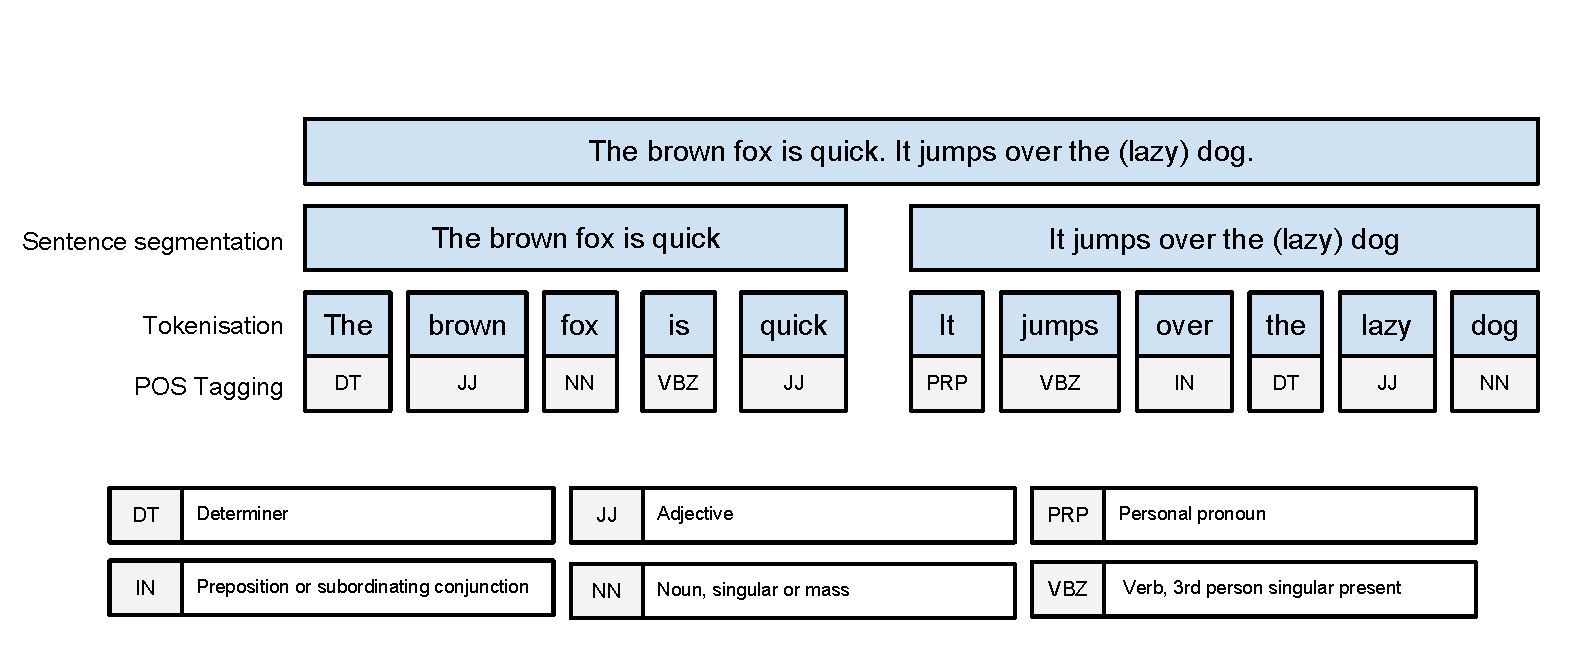
\includegraphics[width=\textwidth]{img/implementation/Tokenisation.pdf}
	\caption{Stepping through the tokenisation process}
	\label{fig:tokenisation}
\end{figure}

\subsection{Named Entity Recognition}

The second half of the keyword extraction process is exclusively concerned with named entities within articles. This is because, intuitively, the names of people, places, events companies and other \textit{things} form a set of strong candidate keywords. Restricting the candidates to entities alone reduces the search space by an order of magnitude when using frequency-based methods for keyword extraction, and bypasses the need for other natural language processing tasks such as stop-word removal and lemmatisation.

Once tokens have been POS tagged, named-entity chunking can be performed, again using NLTK. This process groups tokens into contiguous and non-overlapping \textit{chunks}, where each chunk is a named entity; typically a proper noun or some other noun phrase. It is possible for chunks to contain other chunks (consider the chunk `Bank of England', which contains the chunk `England'), but this is typically undesirable for entity recognition -- where we desire specificity -- so after chunking the tokens, we flatten the chunk structure so chunks cannot be any further decomposed.

At this stage, we have a list of chunks, each of which will be an eventual candidate for becoming a metro line. However, the chunks require some further processing before we can determine whether or not they are significant keywords.

\subsubsection{Substring Matching}
It is common stylistic practice in journalism to refer to the subjects of articles by their surnames. However, to avoid any confusion, the full names of those mentioned will often appear in the title or first few paragraphs of the article. If keyword strength is determined by frequency, then regardless of whether we use tf-idf or tf-pdf, we need every occurrence of an entity to refer to that entity by the same name; preferably the most specific, which is typically the longest.

During this stage of disambiguation, we only consider entities with more than one mention in the source text as candidates. This is because the chunking process can produce false positives by combining unrelated adjectives with valid chunks, but the likelihood of the same false positive being produced twice or more in the same article is low.

Let $P$ denote the set of entities with more than one occurrence in the source article; $S$:
\begin{align*}
P &= \{e\;|\;\text{occurences}(e, S) > 1\}.
\intertext{$\forall (e_1, e_2) \in \{P\times{P}\;|\;$length$(e_1)\;<\;$length$(e_2)\}, $ if $e_1 $ is a substring of $e_2$, we call $e_1$ an \textit{alias} of $e_2$. Let $A$ be the set of alias pairs in $S$;} 
A &= \{(a, e) \;|\;a \text{ is an alias of } e\}
\intertext{We require the first term of every pair in $A$ to be unique, but there is no such constraint for the second term ($e$); this allows multiple aliases to map to the same entity. For example,} 
 & \{(\text{`Zuckerberg'}, \text{`Mark Zuckerberg'}), (\text{`Zuck'}, \text{`Mark Zuckerberg'})\} 
%\intertext{and}
%& \{(\text{`Zuck'}, \text{`Zuckerberg'}), (\text{`Zuckerberg'}, \text{`Mark Zuckerberg'})\}
\intertext{would be unambiguous and therefore valid, but}
 & \{(\text{`Mark'}, \text{`Mark Zuckerberg'}), (\text{`Mark'}, \text{`Zuckerberg'})\}
\intertext{would not be. Let $U$ be the set of unambiguous alias-entity pairs in $S$:}
U &= \{(a, e) \;|\; (a, e)\in{A} \cap \forall(e_1, e_2)\in A, \; a = e_1 \implies e = e_2 \}
\end{align*}

We have a reasonable degree of confidence that for every alias-entity pair $(a, e) \in U$, occurrences of $a$ in the source text can be replaced by $e$, making $e$ a stronger candidate for keyword detection. Pairs in $(a, e) \in A\setminus{U}$, that is, aliases which could map to multiple entities in the source, are disregarded at this stage and left unchanged.  Algorithm \ref{alg:u} illustrates how, given a list of entities, we can find the unambiguous pairs deterministically. 

\begin{algorithm}
\label{alg:u}
 \caption{Finding unambiguous alias-entity pairs}
 \KwData{$names$: a list of recognised entities}
 \KwResult{$U$: the set of unambiguous pairs in $names$}
 $U \gets$ \{\}\;
 \ForEach{$e_1, e_2$ $\in ($names $\times$ names$)$}{
   \If{len($e_1$) $>$ len($e_2$)}{
   	swap($e_1$, $e_2$) \;
   }
  \If(\tcc*[f]{If $e_1$ is a substring of $e_2$}){$e_1 \in e_2$}{
   	\eIf{$e_1 \notin U$}{
   	  $U$[$e_1$] $\gets e_2$ \tcc*[r]{$(e_1, e_2)$ are a candidate pair}
    }{
      delete $U$[$e_1$] \tcc*[r]{$e_1$ is now ambiguous, so remove it}
    }
   }
 }
\end{algorithm}


\subsubsection{Entity Disambiguation with Knowledge Graph}

The process described above is a simplistic approach which only addresses the matching of partial to full name mentions. In comparison, entity disambiguation describes the process of determining the identity of entities in a body of text. Performing this process on the sentence `The UK has voted to leave the EU,' should identify `UK' as 'The United Kingdom' and `EU' as 'The European Union'. As advanced methods for entity disambiguation are both complex and computationally expensive, I did not attempt to implement a formal method for this. 

Instead, the list of recognised entities are queried against Google's publicly accessible Knowledge Graph API, which returns a list of potential results as Schema.org\footnote{http://schema.org is an online hierarchy of types managed by W3C (The World Wide Web Consortium)} types. Knowledge Graph is the service which replaced Freebase in 2015, and currently contains over 70 billion facts \citep{knowledgegraph}.

\cite{EntityDisambiguationForKnowledgeBasePopulation} identify three key challenges in entity linking using knowledge bases; name variations, ambiguity, and absence. Absence describes the lack of a corresponding entry for the entity in the knowledge base, which is not an easily tackled problem. Ambiguity is a consequence of the polysemy of many names and acronyms and requires disambiguation to be performed using more contextual methods. 

Both of these problems are left unsolved in the design and implementation of the system due to scoping constraints. However, naïve substring matching combined with the use of Knowledge Graph and some empirical parametric estimation are enough to disambiguate name variations of all forms (partial matches, abbreviations, and acronyms) to a sufficient degree, and with surprising accuracy.

The key to using Knowledge Graph for disambiguation lies in its most vaguely defined return value. Each result has a score attributed to it by Knowledge Graph, which is an indicator the strength of the match between the entity and the original query. Results are sorted by descending score; the higher the \texttt{resultScore}, the better the match. Although there is no defined upper limit for this value and no official documentation on how the score is derived, comparing the scores of the top two results for a query can provide a measure of certainty, for all but particularly esoteric or unknown entities.

We specify a threshold $\frac{1}{t}$, which is roughly proportional to the likelihood of accepting a false positive match. Then, if dividing the score of the first result by the score of the second yields a number greater than $\frac{1}{t}$, we accept the match. Provisionally we set $t=0.5$; a discussion of how I arrived at this value is provided in the next section.

Using a knowledge base for disambiguation also inadvertently solves another problem I encountered while parsing articles, this time as a result the expositional style of journalistic writing. While keywords are typically nouns or noun phrases, they can also appear in the form of denominal adjectives. These adjectives are derived from nouns; e.g. `French' implies `France' might be a keyword. Denominal adjectives are not amenable to traditional stemming or lemmatising, but querying Knowledge Graph for `French' returns a top match of `France' with a \texttt{resultScore} of 432.42807; more than four times larger than the next result.

Given a list of entities $E$, and top two results of a Knowledge Graph query for each $e \in E$; $R_e(1)$ and $R_e(2)$ with scores $S_e(1)$ and $S_e(2)$ respectively, our aim is to return a set of pairs mapping zero or more entities in $E$ to their disambiguated forms;

\begin{align*}
K &= \bigg\{(e, R_e(1))\;|\;\frac{S_e(1)}{S_e(2)} > \frac{1}{t}\bigg\}
\end{align*}

Algorithm \ref{alg:kg} describes this process. For higher values of $t$, the likelihood of accepting a false positive increases, and for lower values, the likelihood of accepting a false negative increases. For corpora which do not contain references to public figures and place names, choice of $t$ should be empirically tuned against the prevalence of the expected entities.

\begin{algorithm}
\label{alg:kg}
 \caption{Entity disambiguation with Knowledge Graph}
 \KwData{$names$: a list of recognised entities \\ 
 		\hspace{1.2cm}$t$: the acceptance threshold for results, default = 0.5}
 \KwResult{$K$: a set of disambiguation mappings for elements in $names$}
 $K \gets$ \{\}\;
 $T \gets 1\div{t}$\;
 \ForEach{$e \in names$}{
 	$results \gets$ KnowledgeGraphResults($e$)\;
 	\If{len($results$) $>$ 1}{
	   \If{$results$[0].score $\div$ $results$[1].score $> T$}{
	   		$K[e] = results[0].name$\;
	   }
	}
 }
\end{algorithm}

It is unclear what should become of queries that Knowledge Graph only returns a single result for, but in this implementation they are ignored.

\subsubsection{Determining Optimal Values for $t$}

Empirically, I found the best values for $t$ are in the range $0.35 < t < 0.65$, meaning we accept top results which are at least 1.5x-3x higher than the next best candidate. To determine this, I logged all the disambiguation pairs found in 20 articles from the BBC Politics RSS feed, letting $t$ range over \{0.3, 0.5, 0.7, 0.9\}. I then manually classified the pairs as either true or false positives, where a true positive indicates a correctly identified entity, and a false positive is either an incorrectly identified entity or a non-entity which was not identified at all. Figure \ref{fig:dthreshold} shows the results of this investigation.

\begin{figure}[htbp!]
	\centering
	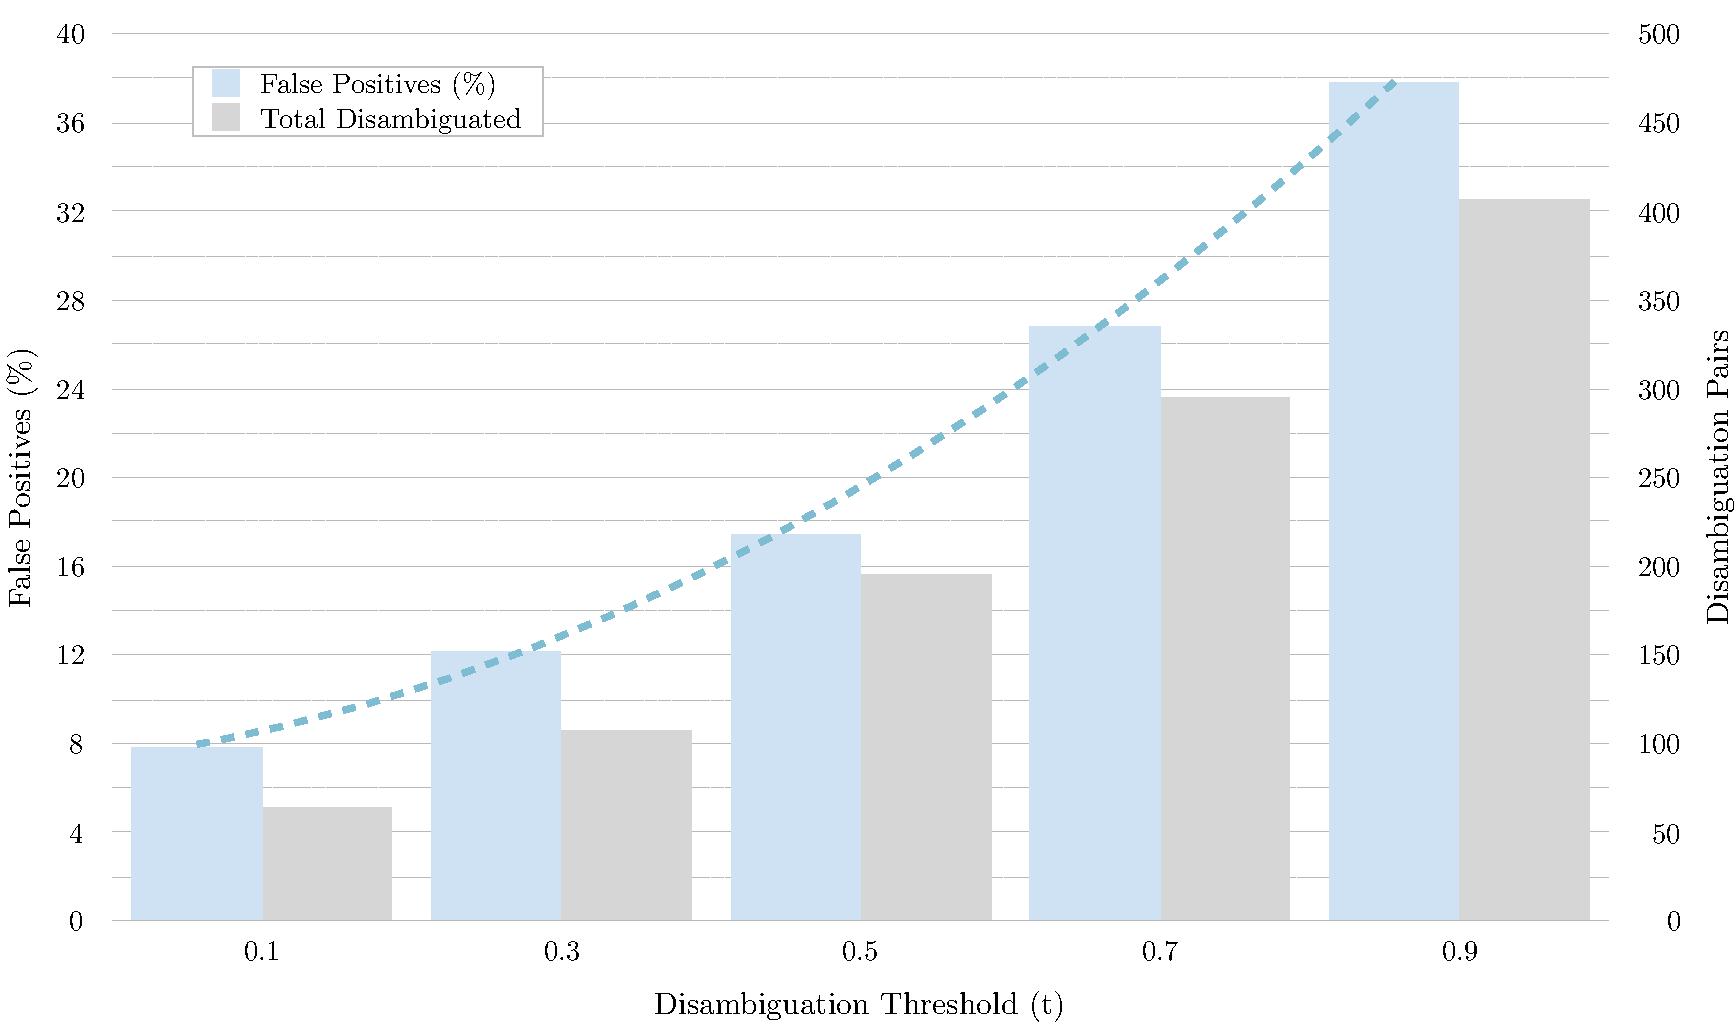
\includegraphics[width=\textwidth]{img/implementation/DisambiguationThreshold.pdf}
	\caption{Disambiguation threshold against pairs found and false positives (\%)}
	\label{fig:dthreshold}
\end{figure}

Although we see a reduction in false positives for smaller values of $t$, the trend-line illustrates that this is a game of diminishing returns; reducing $t$ from 0.3 to 0.1 only reduces the false positives by 4.34\%, but it leads to 43 fewer pairs being identified\footnote{Since it is both extensive and tangential to the focus of the project, raw data for this table can be found at \url{http://bit.ly/DisambiguationThresholding}.}. 

There is a clear trade-off between the accuracy of the disambiguation and the number of false negatives we discard, but the cost of false positives in this case is less than the cost of false negatives. While a false positive could result in unrelated entities appearing as keywords for certain articles, the likelihood of the same false positive appearing with high frequency in enough articles to result in an erroneous metro line is incredibly low. In contrast, the cost of disregarding a false negative could result in articles being left off certain metro lines altogether. It is for this reason that we don't simply choose the value of $t$ which yields the minimum ratio of false positives.

\subsection{Choosing a Term-Weighting Metric for Keyword Ranking}

Given a set of disambiguated entities for every article, the union of which forms a set of candidates keywords or \textit{metro lines} for the collection, we must now determine which keywords are the most relevant. To do this, the two term-weighting methods described in Chapter \ref{c:litreview} will be revisited; tf-idf \citep{tfidf} and tf-pdf \citep{TopicExtractionfromnewsArchiveUsingTFPDFAlgorithm}. Both were implemented in the system so they could be compared directly against each another.

From an implementation perspective, the main difference between these two algorithms are the level at which they operate. tf-idf ranks keywords on a per-article basis, returning a vector of an article's keywords and their corresponding score against the background corpus. In contrast, tf-pdf is specified at corpus level and only returns a single metric for a given word; the sum of its significance across the whole corpus. In tf-pdf, corpuses have one or more \textit{channels}, which contain articles. In our case, channels can be conveniently defined as RSS feeds from different publishers. 

\citeauthor{TopicExtractionfromnewsArchiveUsingTFPDFAlgorithm} argue that tf-pdf is a more suitable metric for news corpora, because it discriminates between articles which originated from the same channel and articles in different channels, allowing keywords which are highly (and uniformly) frequent in one channel to be identified as significant in documents from a different channel. Similarly to tf-idf however, this process can be used to produce a vector of pairs of an article's highest ranked keywords. The actual scores attributed to keywords by either algorithm are not of direct importance, since it is only relative scores we use to construct the keyword vectors.

%\subsubsection{Implementation of tf-pdf Vectorisation}
%
%\begin{itemize}[noitemsep]
%	\item $D$ = The number of channels in the corpus;
%	\item $K_c$ = The total number of terms in channel $c$;
%	\item $F_{tc}$ = Frequency of term $t$ in channel $c$;
%	\item $n_{tc}$ = The number of articles in channel $c$ where term $t$ occurs;
%	\item $N_c$ = The total number of articles in channel $c$.
%\end{itemize}
%\begin{equation}
%	\text{tf-pdf}(t) = \sum_{c=1}^{c=D}\frac{F_{tc}}{\sqrt{\;\sum\limits_{k=1}^{k={K_c}}{F_{kc}}^2}}\times\text{exp}{\bigg(\frac{n_{tc}}{Nc}\bigg)}
%\tag{\ref{eqn:tfpdf}}
%\end{equation}

Regardless of which algorithm is used, the advantage to restricting the set of candidates to named entities becomes quickly apparent. Figure \ref{fig:tokensentities} shows the number of tokens against the percentage of extracted entities for 40 articles from the BBC's Politics RSS Feed.\footnote{http://feeds.bbci.co.uk/news/politics/rss.xml (Accessed: 27/02/2017, Full data in Appendix \ref{tab:entitiestokens})} The interquartile range shows 50\% of articles had entities comprising 5.4\%-8.2\% of their tokens after stop-word removal. With the mean equal to 6.65\%, the implications of this are a search space which can be reduced by a factor of more than ten. Although performance optimisation was not specified in the aims of the project, gains of this nature are still significant.

\begin{figure}[htbp!]
	\centering
	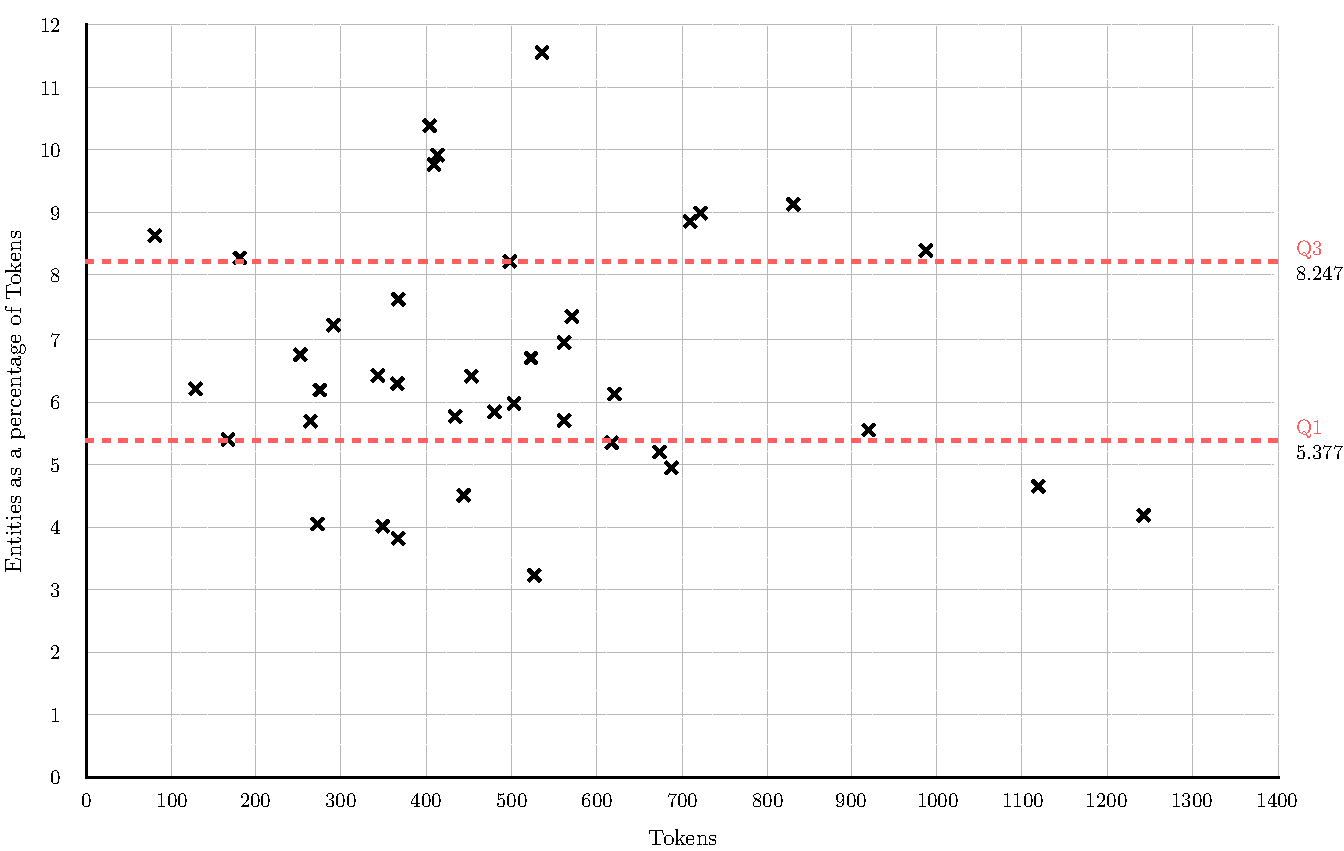
\includegraphics[width=\textwidth]{img/implementation/TokensEntities.pdf}
	\caption{Entities as a percentage of Tokens across 40 BBC Politics articles.}
	\label{fig:tokensentities}
\end{figure}

At this point, given optional user-specified lists of keywords to either \textit{include} or \textit{ignore}, we can filter out or boost the scores of articles which mention these topics, which in the case of \textit{include} will guarantee the keyword is selected as a metro line in the map, as long as it is mentioned in at least two articles. 

The function of the \textit{ignore} set is not to blacklist certain topics, as it will have no effect on articles which contain ignored keywords being placed on other metro lines. Instead, it performs domain specific stop-word removal for metro line candidates, preventing non-useful keywords with inevitably high scores (such as `United Kingdom' for a metro map based on a UK news corpus) from being selected. During implementation, it was found to be useful to automatically append the names of every news publisher (e.g. `The Guardian') in the feeds to the \textit{ignore} set, as well as the names of the feeds themselves. This forces the system to select more specific candidates, even though their scores may be significantly lower.

While implementing the \textit{ignore} functionality that the differing results of using tf-idf and tf-pdf on the same corpus became obvious. Because tf-idf penalises words which appear with low but constant frequency across a number of documents, keywords we intuitively would wish to ignore such as `United Kingdom' are not scored as highly as they would be with tf-pdf. This is in line with the findings of \citeauthor{TopicExtractionfromnewsArchiveUsingTFPDFAlgorithm}; tf-pdf does do a better job at detecting low-frequency keywords which are consistent across many documents. However, this behaviour is exactly the opposite of what we desire from our metro lines; those low-frequency keywords are most likely already known or could be easily inferred by a user reading the map. Therefore, it is my recommendation that tf-idf be given preference in any implementations of this or similar systems, where the names of more specific low-level themes are being sought.

\clearpage

\section{Graph Building}

The key challenge in graph building is generalising the characteristics of a good overview, from both news consumer and metro map user perspectives. It is at this point that a significant difference between this system and the work of \cite{MetroMapsOfScience, GeneratingInformationMaps, InformationCartographyPre} becomes apparent. 

\citeauthor{GeneratingInformationMaps} generated maps in response to a query (such as the name of an event or time) period, meaning the entire map would then be oriented around that query. In contrast, in our system the only query is an implied one; ``What's going on today?" which offers no starting point for choosing metro lines. Instead of a query-based search problem, we have a multi-document summarisation problem. While they were choosing a set of lines to fit a given query, we are concerned with choosing a set of lines which best cover an entire corpus.

\subsection{Extending the Definition of Coverage to Paths}

Our starting point is a corpus of articles and their associated keyword vectors, which form a metro map by \citeauthor{GeneratingInformationMaps}'s definition, but one with too many edges and paths (metro lines) to be readable in practice. Therefore, in order to intelligently prune the number of paths to some fixed upper bound, we need a metric for comparing the relative importance of paths within a corpus.

To do this, we first recall the original definition of document coverage (equation \ref{eqn:doc-coverage} \citep{GeneratingInformationMaps, MetroMapsOfScience, InformationCartographyPre}), where $d$ is a document, $w$ is a keyword, and $\mathcal{W}$ is some normalised measure of term-frequency, such as tf-idf.

\begin{equation}
	cover_{d}(w) : \mathcal{W} \rightarrow [0,1]
	\tag{\ref{eqn:doc-coverage}}
\end{equation}

In order to compare candidate metro lines, we build on this definition of coverage to extend it to paths (Equation \ref{eqn:line-coverage}).

\begin{equation}
	Coverage(\mathcal{P}) = {|\mathcal{P}|}\sum_{d\,\in\,\mathcal{P}}\frac{cover_{d}(\mathcal{P})}{|\{\,p\in{\Pi}\;|\;d \in p,\,p \neq \mathcal{P}\}|}
	\label{eqn:line-coverage}
\end{equation}

Here, the extent to which a path $\mathcal{P}$ covers a document $d$ within a corpus $\mathcal{D}$ is proportional to its tf-idf coverage of that document and inversely proportional to the number of other candidate paths which \textit{also} cover that document. The coverage of the entire corpus by $\mathcal{P}$ is then given the sum of its coverage of the articles along it multiplied by the length of the path, with high coverage being desirable.

It is important to note that although with the final multiplication we show preference to longer metro lines, the objective of the system is not simply to maximise the number of articles which are included on the generated maps. This could easily be achieved by choosing the most nonspecific universal keywords as metro lines, but the resulting map would be uninformative and would most likely do nothing to counter news overload. It is in the nature of summarisation that not all information can be preserved, and in doing this kind of graph selection, the information lost is those articles which don't form links to the significant topics within the corpus.

%This means tf-idf is preferable to tf-pdf, because while tf-idf is really good at identifying high-level topics which cover a lot of articles, it can cover those articles very poorly and generate a) too few lines, which; b) all run adjacent to each other anyway (see the next section).

\subsection{Penalising Affinity}

The principle of topic connectivity was the basis for choosing the metro map visualisation. Without it, we have simply generated a set of two-dimensional timelines with no contextual links. However, maps which are overly connected will quickly become unusable. In particular, maps where multiple lines runs adjacently through more than two nodes (see figure \ref{fig:lowaffinity}) a sign of poor line choice. This is not simply hyper-connectivity, but correlation between two or more lines, often resulting from keywords which are semantically close.

\begin{figure}[htbp!]
	\centering
	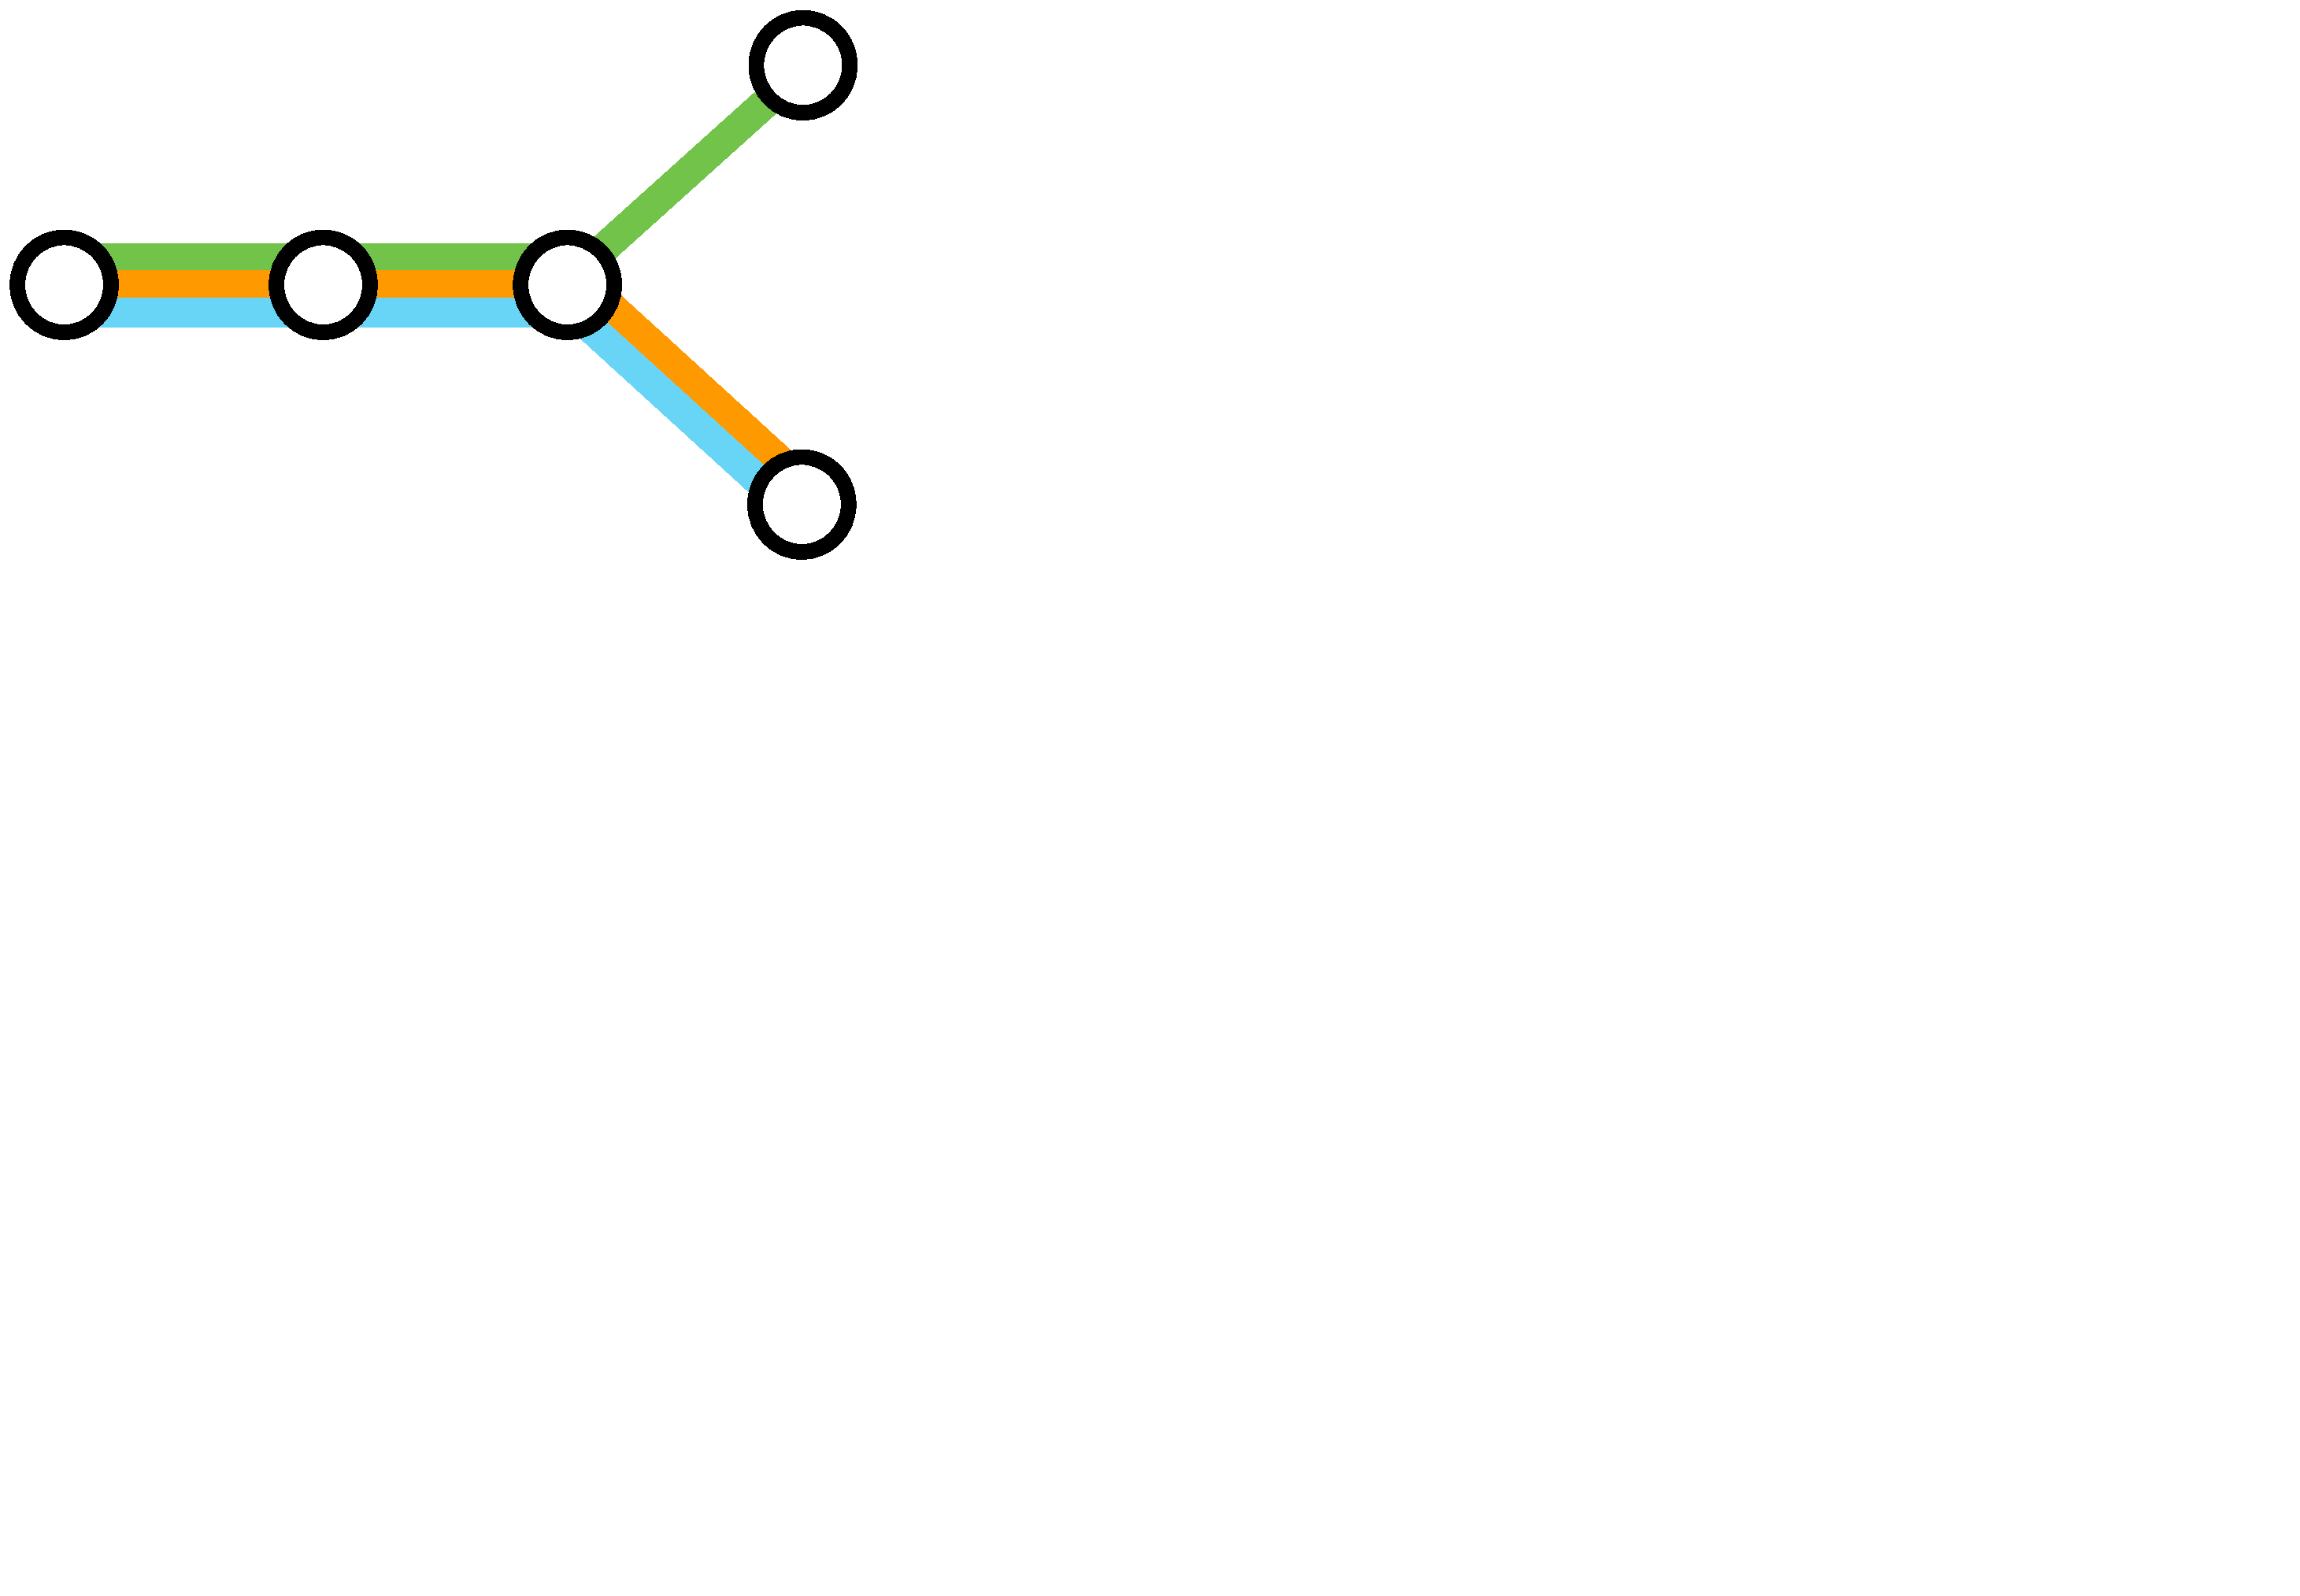
\includegraphics[width=.5\textwidth]{img/implementation/lowaffinity.pdf}
	\caption{An example of three metro lines, each with high affinity.}
	\label{fig:lowaffinity}
\end{figure}

We call this function of two lines their \textit{affinity}, and define the affinity of a single line as the sum of its affinities over the set of paths, excluding itself.

\begin{equation}
	Affinity(\mathcal{P}) = \frac{1}{|\mathcal{P}|} \sum_{p\,\in{\,\Pi}} 2^{|\{\,d\,|\,d\,\in\,{\mathcal{P}}\,\cap\,d\,\in\,{p},\,p\,\neq\,\mathcal{P}\}|}
\end{equation}

The affinity of two lines is defined as the number of articles they have in common, raised as a power of two. The effect of the power is illustrated in Figure \ref{fig:abcaffinity}. On the right, line $a$ (orange) which shares one article with line $b$ (green) and another with line $c$ (blue) does not indicate as strong a correlation as on the left, where $a$ shares two articles with $b$ and none with $c$. As with line coverage, we penalise shorter lines.

\begin{figure}[htbp!]
	\centering
	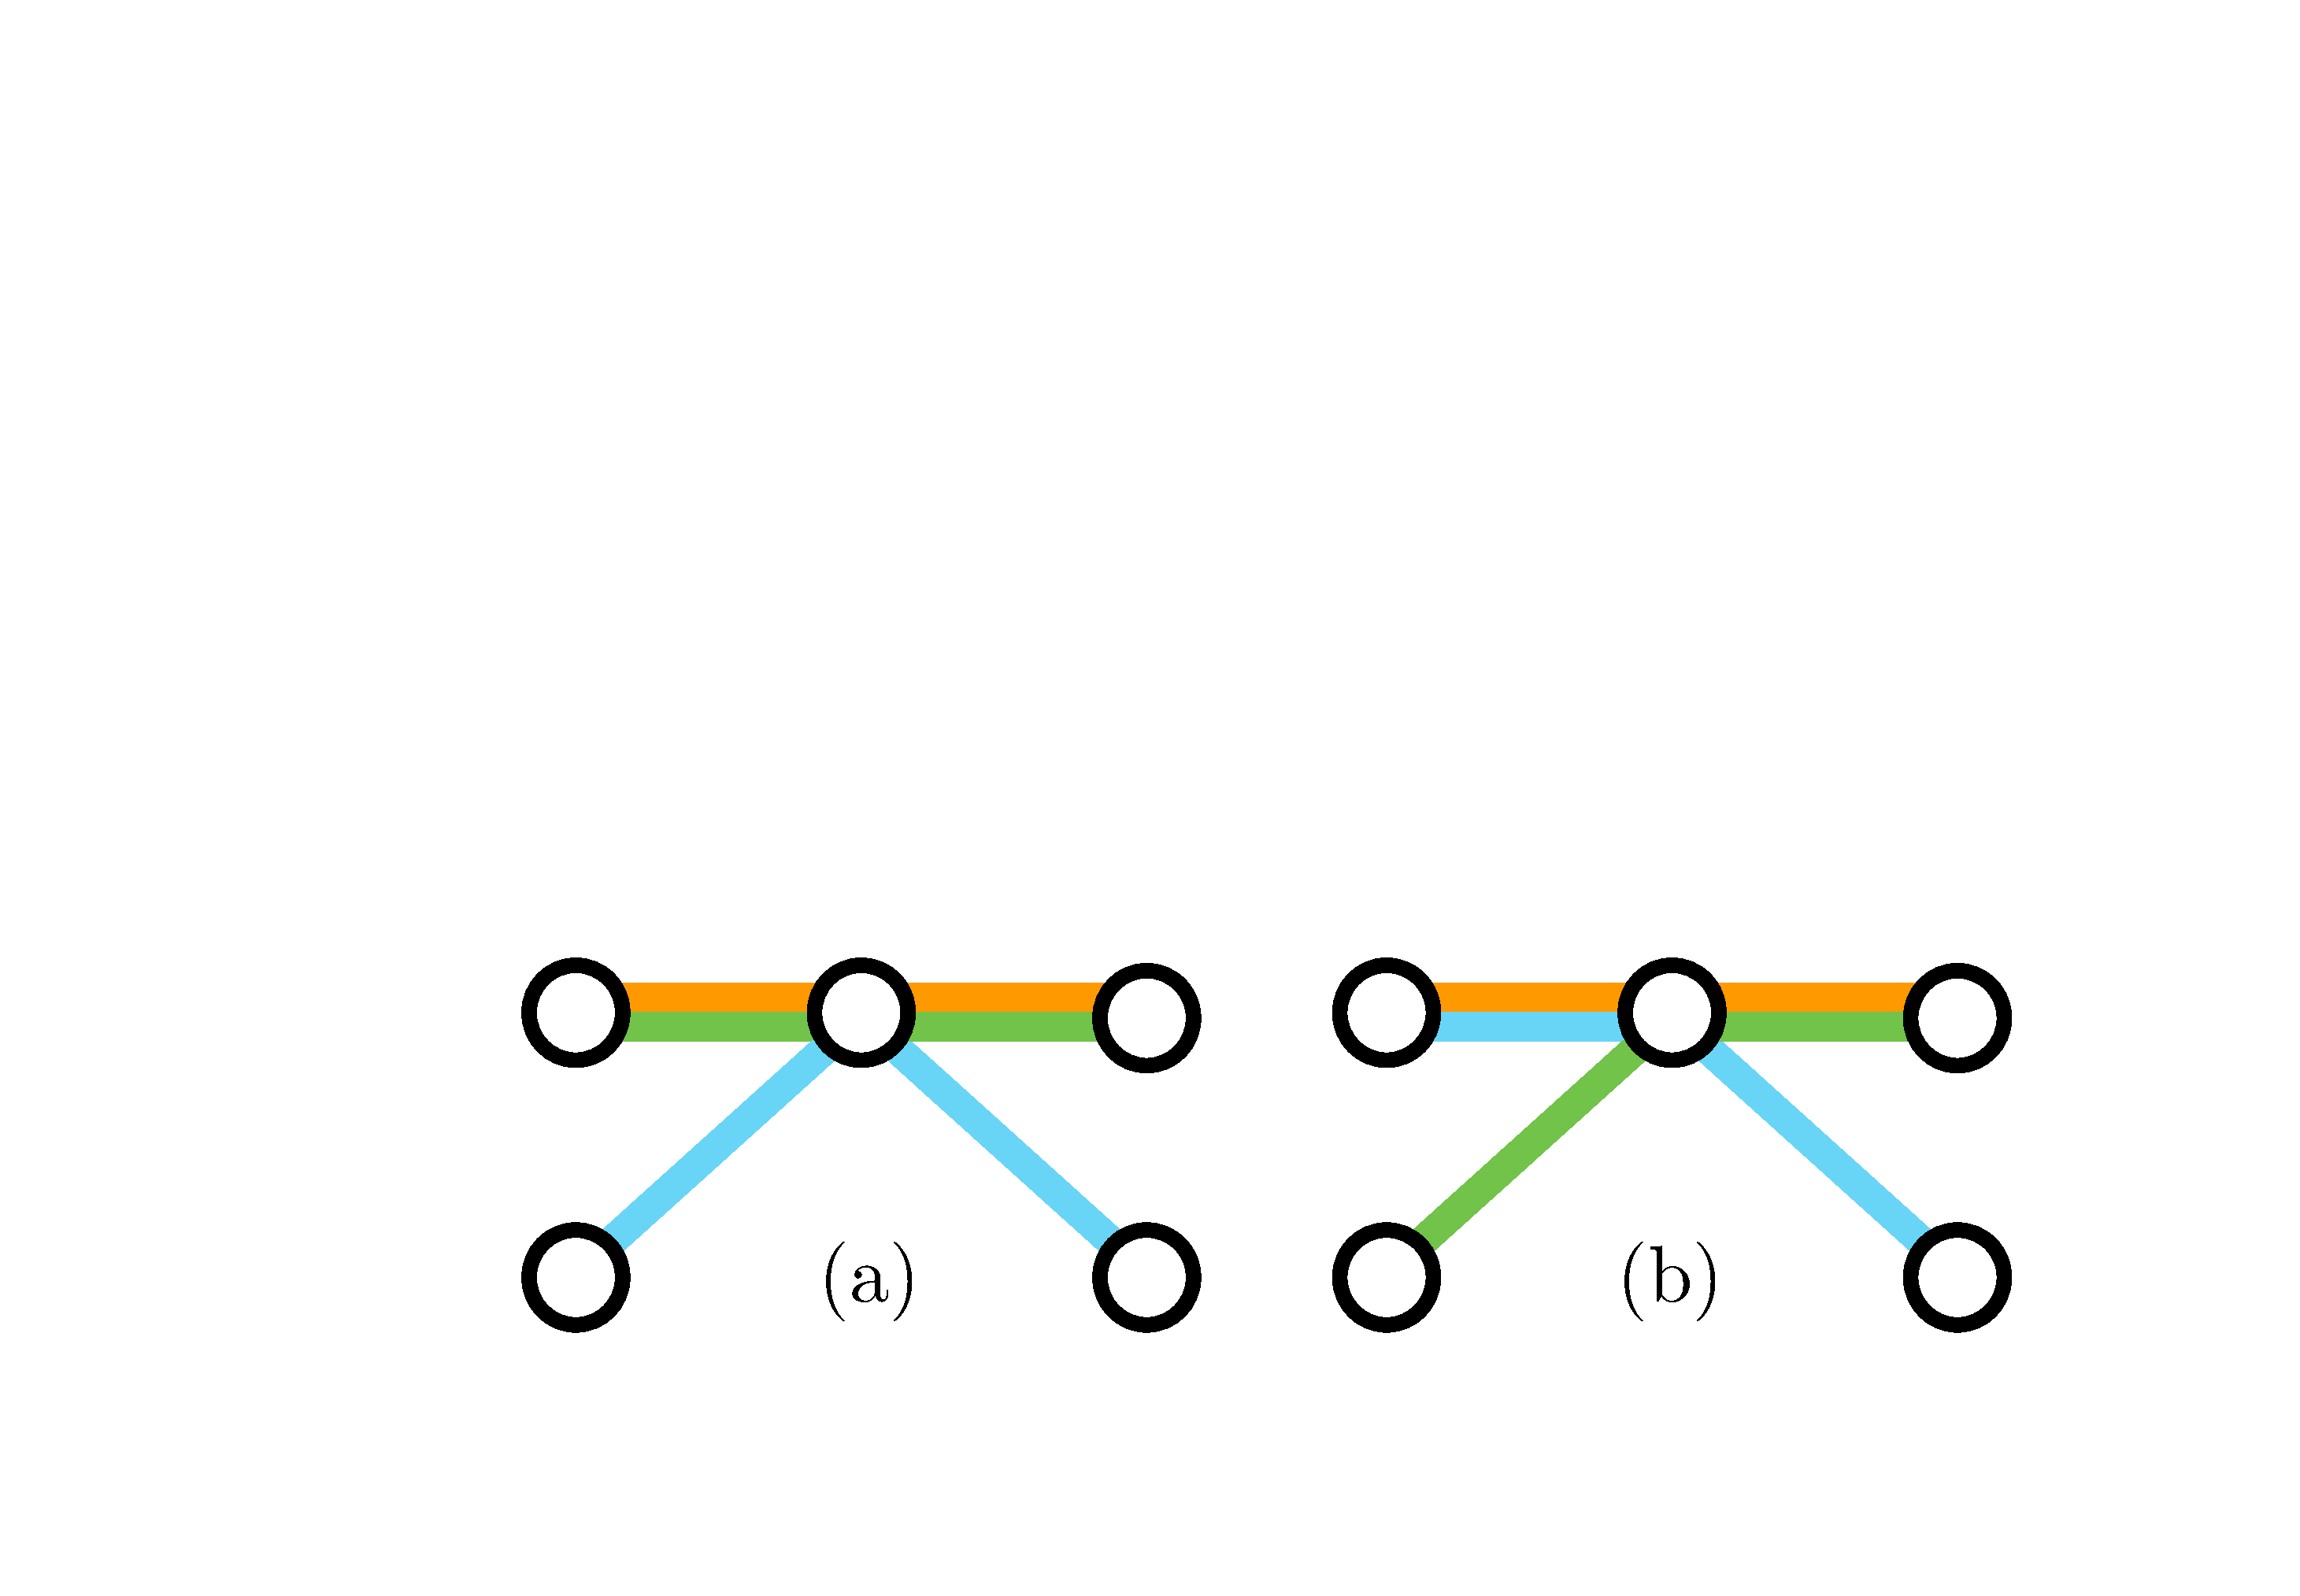
\includegraphics[width=\textwidth]{img/implementation/abcaffinity.pdf}
	\caption{`Run-on' affinity (left) is penalised more heavily than `one-off' affinity (right).}
	\label{fig:abcaffinity}
\end{figure}

Since metro lines should have both high line coverage and low affinity, we can compute a score for every path by dividing the two composite measures (Equation \ref{eq:score}).
\begin{equation}
	LineScore(\mathcal{P}) = \frac{Coverage(\mathcal{P})}{Affinity(\mathcal{P})}
	\label{eq:score}
\end{equation}

Sorting the list of candidates by descending score and filtering out those candidates which contain too few articles to be beneficial, we can then take the top $n$ from the range $7 \leq\;n\;\leq 12$, to become the metro lines in our map. Any article which contains the name of a metro line in its keyword vector will be represented as a station, and articles with more than one will be represented as interchanges.

\subsection{Coherence}
The last metric proposed by \citeauthor{GeneratingInformationMaps} is the one which presented the greatest conflict with the predefined scope of the system. For all but the most rapidly unfolding stories, forming a coherent chain of articles on one topic or event is not possible when only considering a single day's news. \citeauthor{GeneratingInformationMaps} had the advantage of assuming any topic well-known enough to be queried against their system would most likely be made up of a coherent chain of events, such as the Greek debt crisis or Brexit. In contrast, at a daily summarisation level, often no such chains exist; many articles exist in isolation or instead represent the \textit{beginning} of a potential future storyline. 

Given a large enough background corpus, it would be possible to link the day's summary back in time to older articles, extending metro lines further back to support the \textit{zoom and filter} or \textit{details-on-demand} processes. A great deal of potential lies in this idea, as it could provide the story resolution the participants in the \cite{anewmodelfornews} study craved, allowing users to explore further back in time along individual metro lines while still centring itself around the most recent news. Unfortunately however, this is not something I could have achieved within the assigned timescale. 


\subsection{Serialisation}
The intermediate stage of the pipeline between graph building and map drawing is purely an issue of implementation, with few design choices to be made. Starting with the Python representation of the metro map, we group articles by metro line to be serialised, along with their metadata and summaries, to JSON. This JSON is then copied into a preexisting JavaScript file which is responsible for representing and drawing the graph using D3.js, and the contents of the JavaScript file are embedded as a script in an HTML file, which contains general template markup for the page. 

The main advantage to this process is that it results in a single file, meaning the resultant visualisations are as portable, shareable and platform independent as the news they were derived from. A secondary advantage is that the JSON accepted by D3 is standard and could easily be fed into a different JavaScript graphing library in the case of a more suitable alternative being written, with no change to the core Python software. The core software itself could also be hosted as a web app which serves the map HTML files, removing the need for client-side processing or installation.

\clearpage
\section{Map Drawing}

The metro map layout problem, that is, determining whether an optimal planar embedding exists for a map and a set of hard constraints which include drawing straight octilinear lines, was proven to be NP-Hard by \cite{AutomatedDrawingOfMetroMaps}. The authors present a mixed-integer program (MIP) approach to metro map layouts, which both guarantees an octilinear layout and avoids falling into local maxima (unlike \citeauthor{AutomaticMetroMapLayoutThesis}'s), but not in polynomial time.

At the time of writing, there are no public domain algorithms or open-source libraries for generating automatic metro map layouts, in any language. Those which have been proposed in academia \citep{AutomaticMetroMapLayoutThesis, AutomatedDrawingOfMetroMaps} are too complex to implement given the current timescale, and all require NP-Hard optimisation techniques. To overcome this, a heuristic approach derived from the work of \citep{AutomaticMetroMapLayoutThesis, AutomaticMetroMapLayout, WhichAesthetic} will be detailed.

In this section of the pipeline, we are no longer concerned with the contents of articles or the entities they reference. The map drawing context marks a shift in the terminology from the previous stages of the pipeline to the domain of graph drawing, but many terms have a one-to-one correspondence. A list of definitions is given below, and in addition we recall \citeauthor{GeneratingInformationMaps}'s definition of a metro map from Chapter \ref{c:litreview}, which ties the terms together.

\addtocounter{definition}{-1}
\begin{definition}{}
A metro map $\mathcal{M}$ is a pair $(G, \Pi)$, where $G=(V, E)$ is a directed graph and $\Pi$ is a set of paths, or \textit{metro lines} in $G$. Each $e \in E$ must belong to at least one metro line.
\end{definition}
\vspace{-0.5cm}
\begin{figure}[htbp!]
	\centering
	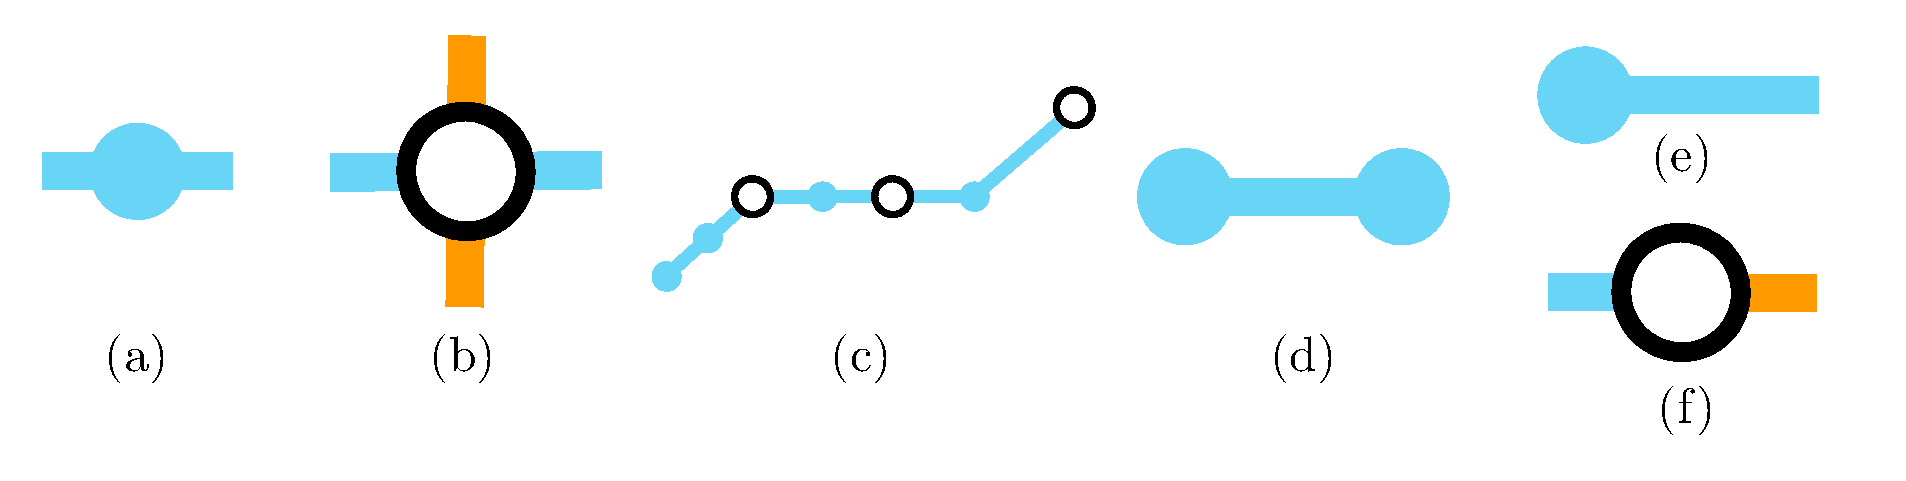
\includegraphics[width=\textwidth]{img/implementation/mapdefinitions.pdf}
	\vspace{-0.5cm}\caption{Left-to-Right: A station (a), an interchange (b), a metro line (c), a link (d), a terminus (e) and a non-terminus station (f).}
	\label{fig:mapdefinitions}
\end{figure}
\begin{description}[leftmargin=7em,style=nextline]
	\item [Station] A single article $v \in V$, represented by a node in the graph. If $v$ has more than two incident edges, i.e an article which spans more than one topic in the graph, it is called an \textit{interchange}.
	\item [Metro Line] A contiguous named path $p \in \Pi$ which is incident to two or more nodes, represented by a line of single colour. Metro lines are composed of \textit{links}.
	\item [Link] A direct edge $e \in E$ between two nodes, which does not pass through any other node. In contrast to \citeauthor{GeneratingInformationMaps}'s definition, here, links must belong to \textit{exactly one} metro line. The case of two lines running side-by-side through the same two nodes is represented by two distinct links. This difference is due only to an implementation detail of the graphing library chosen.
	\item [Terminus] A node with only one incident edge. This is not the definition of a terminus in the sense of the underlying metaphor, since by our definition, a station which is the terminus for two lines (see Figure \ref{fig:mapdefinitions}.f) is no longer categorised as a terminus at all. Instead, the definition requires that the position of a terminus only determine the position of a single link in the graph.
\end{description}

We now turn our attention to transforming the metro map structure into a planar embedding of stations and the metro lines which connect them. As we have previously observed, not all graph layouts were created equal, and the aesthetic quality of a graph-based visualisations has a notable influence on their usability and ease of interpretation \citep{TheBasisForGraphDrawingAlgorithms, WhichAesthetic, AutomaticMetroMapLayoutThesis, AutomaticMetroMapLayout}. 

In \citeauthor{AutomaticMetroMapLayoutThesis}'s words: ``[The] visualisation process is deeply rooted in the human interpretation of the graph as a structure and as such, the quality of the aesthetics of a particular drawing of a graph are very important.'' \citep[p.24]{AutomaticMetroMapLayoutThesis}

We therefore devote a significant amount of thought to optimising the visual quality of the generated metro maps by revisiting \citeauthor{AutomaticMetroMapLayoutThesis}'s aesthetic criteria for layouts, discussed in Chapter \ref{c:litreview}. We justify which of these apply to our visualisations, and for those which are, we detail the methodology used to implement them.

\subsection{\citeauthor{AutomaticMetroMapLayoutThesis}'s Criteria Metro Map layouts}

The set of rules and criteria defined by \cite{AutomaticMetroMapLayoutThesis} form a complex multicriteria optimisation function. Starting with an initial layout, nodes are embedded on a square grid of finite size, and iteratively moved to maximise the node movement criteria, as long as movement does not violate one of the node movement rules.

It should be noted that the function also applies to the positioning of labels and the maximum of a set of label movement criteria alongside the node movement criteria, but as visualisations are unlabelled, these will not be described.

As previously discussed, there are six node movement criteria, which -- using the metro map-specific terms defined above -- are as follows:
\begin{itemize}
	\item\textbf{Angular Resolution}: Maximise the angle of incident links on the same metro line at each station. As \cite{WhichAesthetic} found satisfying this criteria had no statistical effect on task performance, this will not be a priority\footnote{However, as angular resolution comes as a natural consequence of maximising line straightness, it is not disregarded completely during implementation.}.
	
	\item\textbf{Edge Length}: Keep all links approximately the same length. This is a criterion which can be implemented by setting a soft constraint using the graphing library, but it will not be considered beyond this constraint.
	
	\item\textbf{Balanced Edge Length}: Keep links incident to a given station approximately the same length. While it would be possible to implement this as another soft constraint, there is no evidence that it would significantly improve usability, so this will not be considered.
	
	\item\textbf{Edge Crossings}: Minimise the number of link crossings. \citeauthor{WhichAesthetic} found this to be the most significant factor in determining task performance, therefore it will be considered.
	
	\item\textbf{Line Straightness}: Maximise the collinearity of links on the same metro line. \citeauthor{WhichAesthetic} found this criterion to be somewhat beneficial to task performance, so this is both a realistic and justified constraint which will be considered. 
	
	\item\textbf{Octilinearity}: Draw links at multiples of 45$^{\circ}$. Although \citeauthor{WhichAesthetic} found orthogonal graphs to be insignificant factors on task performance, there is a strong argument that the familiarity of the metro map metaphor hinges on certain similarities being preserved. Octilinearity is a noticeable design feature in the metro maps of the world, and therefore should be attempted in our visualisations.
\end{itemize}

We therefore consider minimising edge crossings to be the highest weighted criterion, followed jointly by maximising line straightness and octilinearity.

\subsection{Initial Force-Directed Positioning}

A major difference between the maps generated using this system and maps representing real transit networks is the lack of ``real'' starting positions we have for stations. While the freedom to move points around without having to preserve their relative positioning removes one layout constraint, finding a set of starting positions for the map layout which define a planar embedding with minimal line crossings is non-trivial. 

As \citeauthor{AutomaticMetroMapLayoutThesis} notes, ``This [difficulty] is due to our method being based on optimising an existing layout: if the initial embedding is not adequate, then our method may struggle to produce an acceptable optimisation.''\cite[p.210]{AutomaticMetroMapLayoutThesis}. One solution he suggests is to generate positions using a force-directed algorithm; a class of algorithms which simulate the forces of real physical motion to position nodes in a graph, with minimal edge crossings and approximately uniform edge lengths \citep{springembedders}. The downside to using a force-directed approach is that initial positioning and therefore the final map layout becomes nondeterministic. 

D3.js includes an optimised implementation of \possessivecite{forcedirected} force-directed layout algorithm, and provides several parameters which can be used to alter the forces applied to some or all of the nodes in the graph. The two forces we will adjust to optimise the force-direction for metro maps are as follows:
\begin{itemize}
\item\texttt{force.charge([charge])}\footnote{\url{https://github.com/d3/d3-3.x-api-reference/blob/master/Force-Layout.md\#charge}}\par
	\textit{Charge} specifies the force of attraction between nodes, with negative values causing nodes to repel each other. In order to minimise crossings, this should be a large negative value, particularly for nodes which of higher degrees, which will be surrounded by more edges. We therefore set charge to -500 for nodes with weight $>$ 1, and -300 otherwise. 

\item\texttt{force.alpha([alpha])}\footnote{\url{https://github.com/d3/d3-3.x-api-reference/blob/master/Force-Layout.md\#alpha}}\par
	\textit{Alpha} is the graph's cooling parameter, decaying as the simulation converges on a stable layout. As the temperature falls, node movement slows down, and eventually alpha will drop below a threshold which pauses the simulation, preventing further movement. 
\end{itemize}

Unfortunately, the implementation of \texttt{d3.layout.force} lacks any further mechanism for detecting or reducing line crossings due to the computational expense of the best known algorithms (this subproblem is also NP-Hard). Even if line crossings could be detected, it is likely that the topology of certain graphs generated would make it impossible to find a planar embedding with no crossings.

The parameter \texttt{force.alpha} is re-evaluated every time the simulation is advanced by a single step, which happens approximately 60 times per second. Since our aim is to generate an initial layout with minimal line crossings which will result in the best possible map, we can constantly vary \texttt{force.alpha} based on the quality of the map as its stations are repositioned. Therefore, if the stations settle into a map layout with desirably high octilinearity and good line straightness, the energy of the graph will be reduced such that it is impossible for the embedding to change. Likewise, if the stations start repelling each other in a way that worsens line straightness and octilinearity, the system will have its energy increased and will be more likely to move out of the undesirable state.

The measure of quality that we use to adjust \texttt{force.alpha} is function of the two remaining chosen aesthetic criteria; octilinearity and line straightness. The means by which these two properties are calculated are described in the following sections.

\subsubsection{Octilinearity}

Octilinearity (Equation \ref{eqn:octilinearity} \citep{AutomaticMetroMapLayoutThesis}) penalises lines which are not drawn at multiples of 45$^{\circ}$ angles; the further the gradient of a link in the graph is from a multiple of 45$^{\circ}$, the higher its octilinearity. Lower values are desirable, with zero indicating a graph is entirely octilinear. 

\begin{equation}
	\text{octilinearity}(G) = \sum_{u, v\in E}\bigg|sin\;4\,\bigg(tan^{-1}\frac{|u.y - v.y|}{|u.x - v.x|}\bigg)\bigg|
\label{eqn:octilinearity}
\end{equation}

\begin{figure}[h]
\centering
\begin{minipage}{.4\textwidth}
  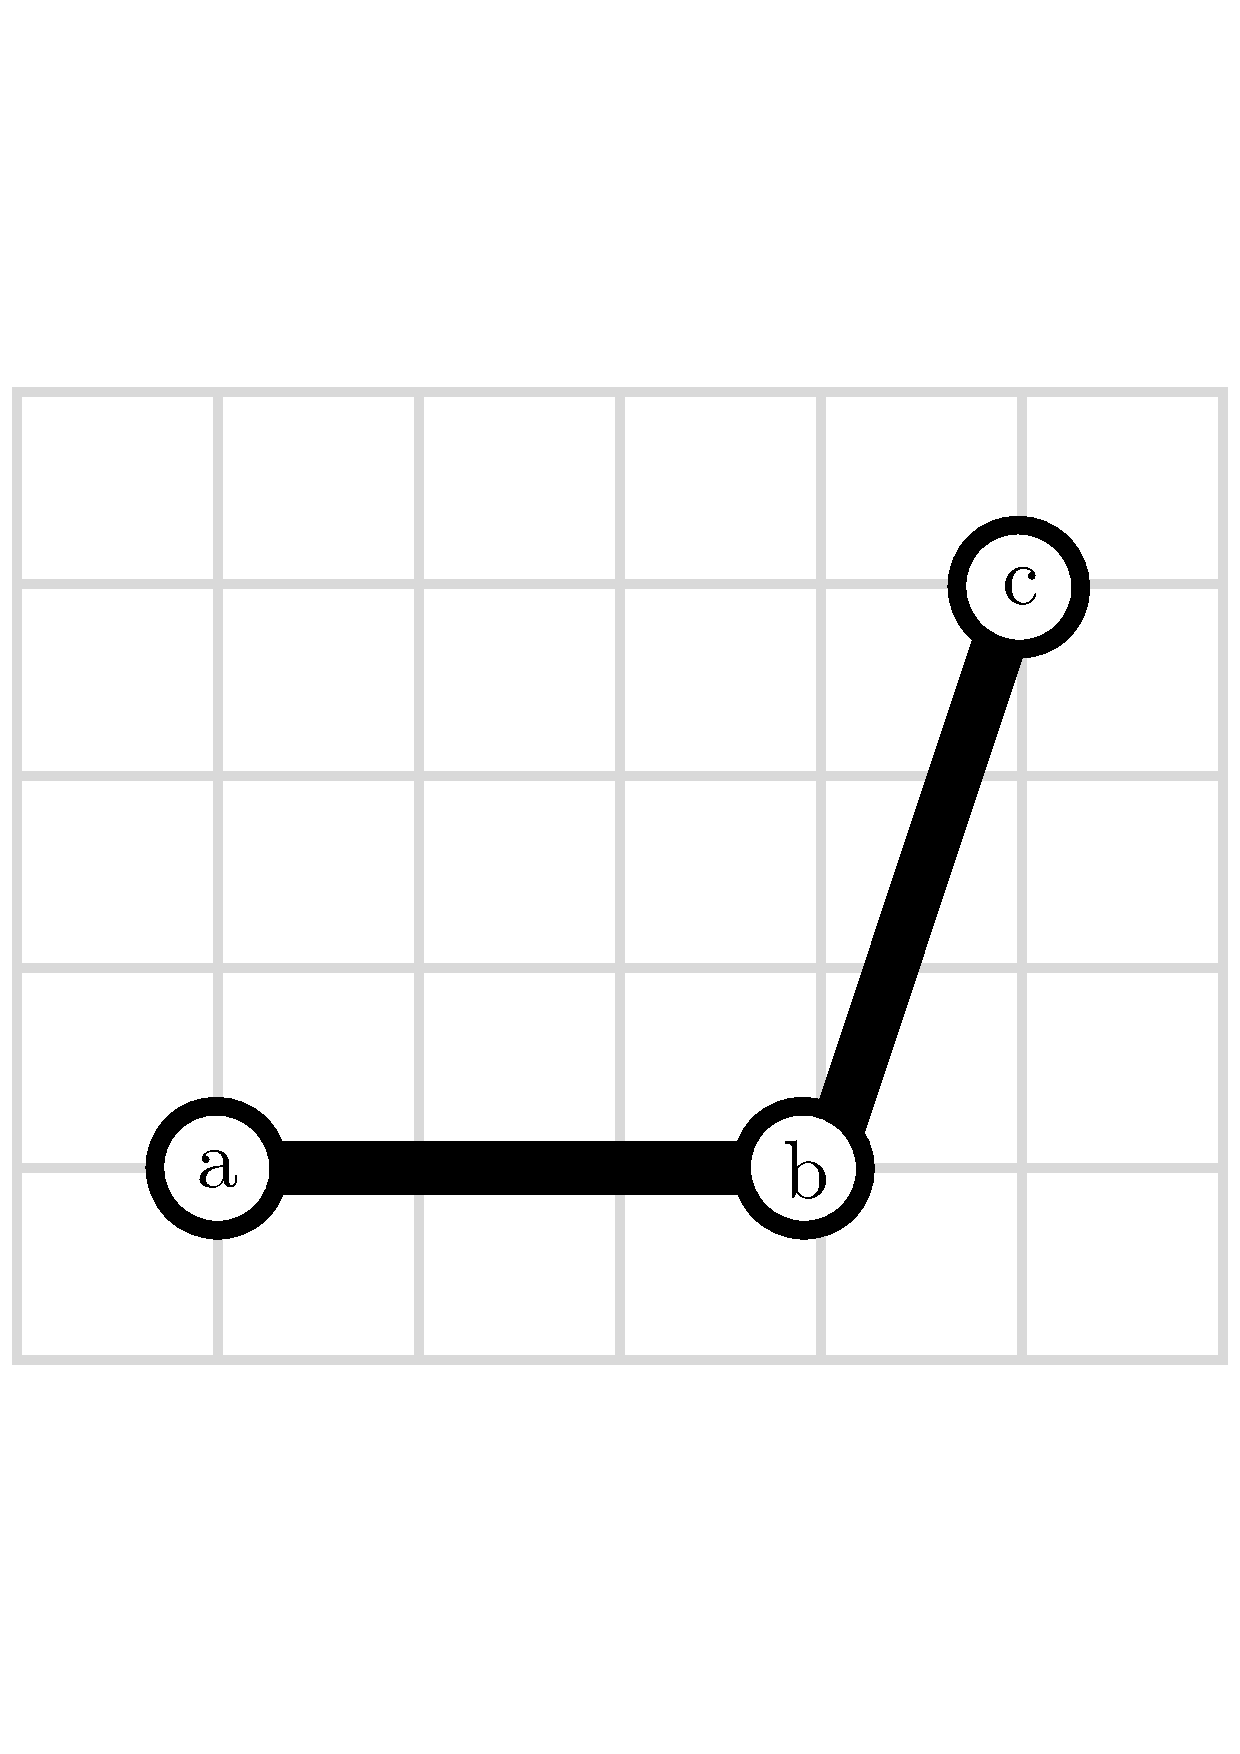
\includegraphics[width=.9\linewidth]{img/implementation/octilinearity.pdf}\caption{Octilinearity Calculation\label{fig:octilinearity}}
  \end{minipage}\hspace{0.5cm}\begin{minipage}{.55\textwidth}
We can calculate the octilinearity of the graph in Figure \ref{fig:octilinearity} (left) as follows, taking positions relative to $(0, 0)$ in the bottom left corner. Algorithm \ref{alg:octilinearity} describes this calculation.
$$\begin{aligned}
\text{octilinearity}(a, b) &= |sin\;4\,(tan^{-1}\frac{|1 - 1|}{|4 - 1|})| = 0 \\
\text{octilinearity}(b, c) &= |sin\;4\,(tan^{-1}\frac{|4 - 1|}{|5 - 4|})| = 0.96 \\[0.1cm]
\text{octilinearity}(a, b, c) &= 0 + 0.96 = 0.96
\end{aligned}$$
\end{minipage}
\end{figure}

There is a caveat to this formula which goes unmentioned by \citeauthor{AutomaticMetroMapLayoutThesis}, but which is necessary to emphasise as a detail of implementation. In the case where $u.x - v.x = 0$, we take octilinearity to be zero, as this value indicates a straight vertical line. Otherwise, attempting to calculate the inverse tangent of a fraction whose denominator is zero (this is mathematically valid, as the principle value of $\tan^{-1}\infty$ is $\frac{\pi}{2}$), which would result in undefined behaviour.\\
\begin{algorithm}
\label{alg:octilinearity}
 \caption{Calculating Map Octilinearity}
 \KwData{$\mathcal{M}$: a metro map $(G=(V, E), \Pi)$}
 \KwResult{$oct \in \mathbb{Q}, 0 \leq oct \leq \frac{24}{25}|E|$: the octilinearity of $\mathcal{M}$}
 $oct \gets 0$ \;
 \ForEach{$e \in E$}{
   $\delta_x \gets |e.source.x - e.target.x|$ \;
   $\delta_y \gets |e.source.y - e.target.y|$ \;
   
   \uIf{$\delta_x = 0 \cup \delta_y = 0$}{
   	 $slope \gets 0$ \tcc*[f]{This avoids a potential division by zero.}}
   	 \Else{
   	  $slope \gets \dfrac{\delta_y}{\delta_x}$ 
    }
   $\theta \gets |sin(4\times{} tan^{-1}(slope))|$ \;
   $oct \gets oct + \theta$ \;
}
\end{algorithm}

\subsubsection{Line Straightness}

The line straightness (Equation \ref{eqn:linestraightness} \citep{AutomaticMetroMapLayoutThesis}) criterion is defined as the sum of every `turn' a metro line makes between its first and last stations, where a turn is measured as the angle between the new link direction and the continuation of the previous direction. The global line straightness is simply the sum of the straightness of every metro line in the map, and as with octilinearity, lower values are preferred.

\begin{equation}
	\text{lineStraigtness}(G) = \sum_{p\,\in{\Pi}}\sum_{u, v\in p} \theta(u, v)
\label{eqn:linestraightness}
\end{equation}

\begin{figure}[h]
\centering
\hspace{-0.5cm}\begin{minipage}{.5\textwidth}
  \centering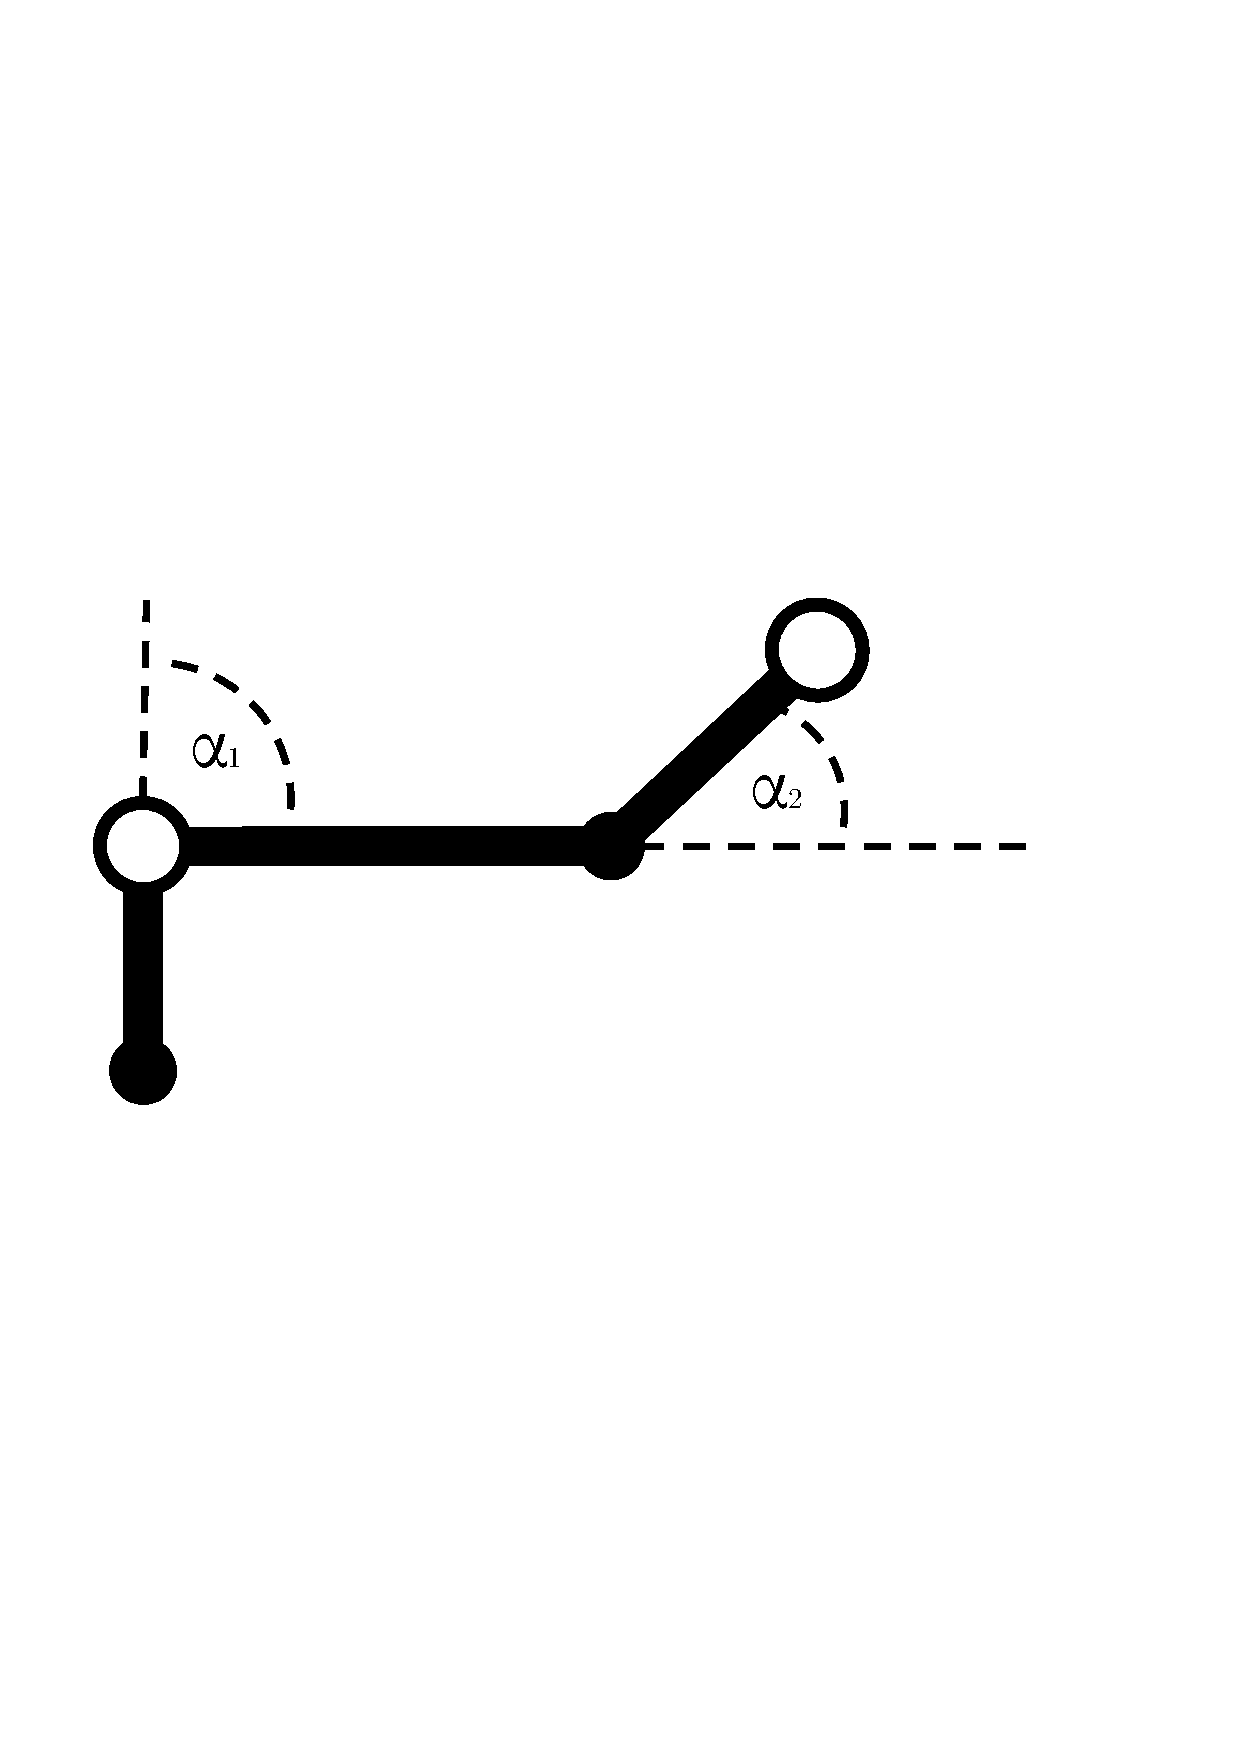
\includegraphics[width=.8\linewidth]{img/implementation/linestraightness.pdf}\caption{Line Straightness Calculation\label{fig:linestraightness}}
  \end{minipage}\hspace{0.5cm}\begin{minipage}{.5\textwidth}
The line straightness of the graph in Figure \ref{fig:linestraightness} (left) is therefore $\alpha_1 + \alpha_2$, where the values of $\alpha_1$ and $\alpha_2$ can be found geometrically from the direction of the links (Algorithm \ref{alg:ls}).
\end{minipage}
\end{figure}

\begin{algorithm}
\label{alg:ls}
 \caption{Calculating Map Line Straightness}
 \KwData{$\mathcal{M}$: a metro map $(G=(V, E), \Pi)$}
 \KwResult{$ls \in \mathbb{Q}, ls > 0$: the line straightness of $\mathcal{M}$}
 $ls \gets 0$ \;
 \ForEach{$p \in \Pi$}{
 	\tcc{Greedily iterate over all 3-tuples of adjacent stations on $p$}
   \ForEach{$(a, b, c) \in p$}{
   \vspace{0.15cm}
   $v_1 \gets \dfrac{\overrightarrow{ab}}{|\overrightarrow{ab}|}$ ; $v_2 \gets \dfrac{\overrightarrow{bc}}{|\overrightarrow{bc}|}$ ;\tcc*[f]{Normalise the two vectors to unit length}
   \vspace{0.15cm}
   $\theta \gets cos^{-1}(v_1.x\times v_2.x + v_1.y\times v_2.y)$ ;\tcc*[f]{Find the angle between links}
   $ls \gets ls + \theta$ \;
   }
}
\end{algorithm}

Empirically, we found the best results came from weighting octilinearity and line straightness equally when using them to set \texttt{force.alpha}, but this could be refined through further investigation. We take the sum of the natural log of both values, to ensure that small improvements to already low values for either criterion are rewarded.

\subsection{Heuristic Refinement}

Once all stations have been assigned their starting positions, we can start incrementally moving them to improve the quality of the map. The first step is to discretise the search space for station positions, by \textit{snapping} stations to intersections on a large grid. We found the optimal size for this grid to be $\frac{n}{4}\times\frac{n}{4}$ for a map containing $n$ stations. 
\begin{figure}[htbp!]
	\centering
	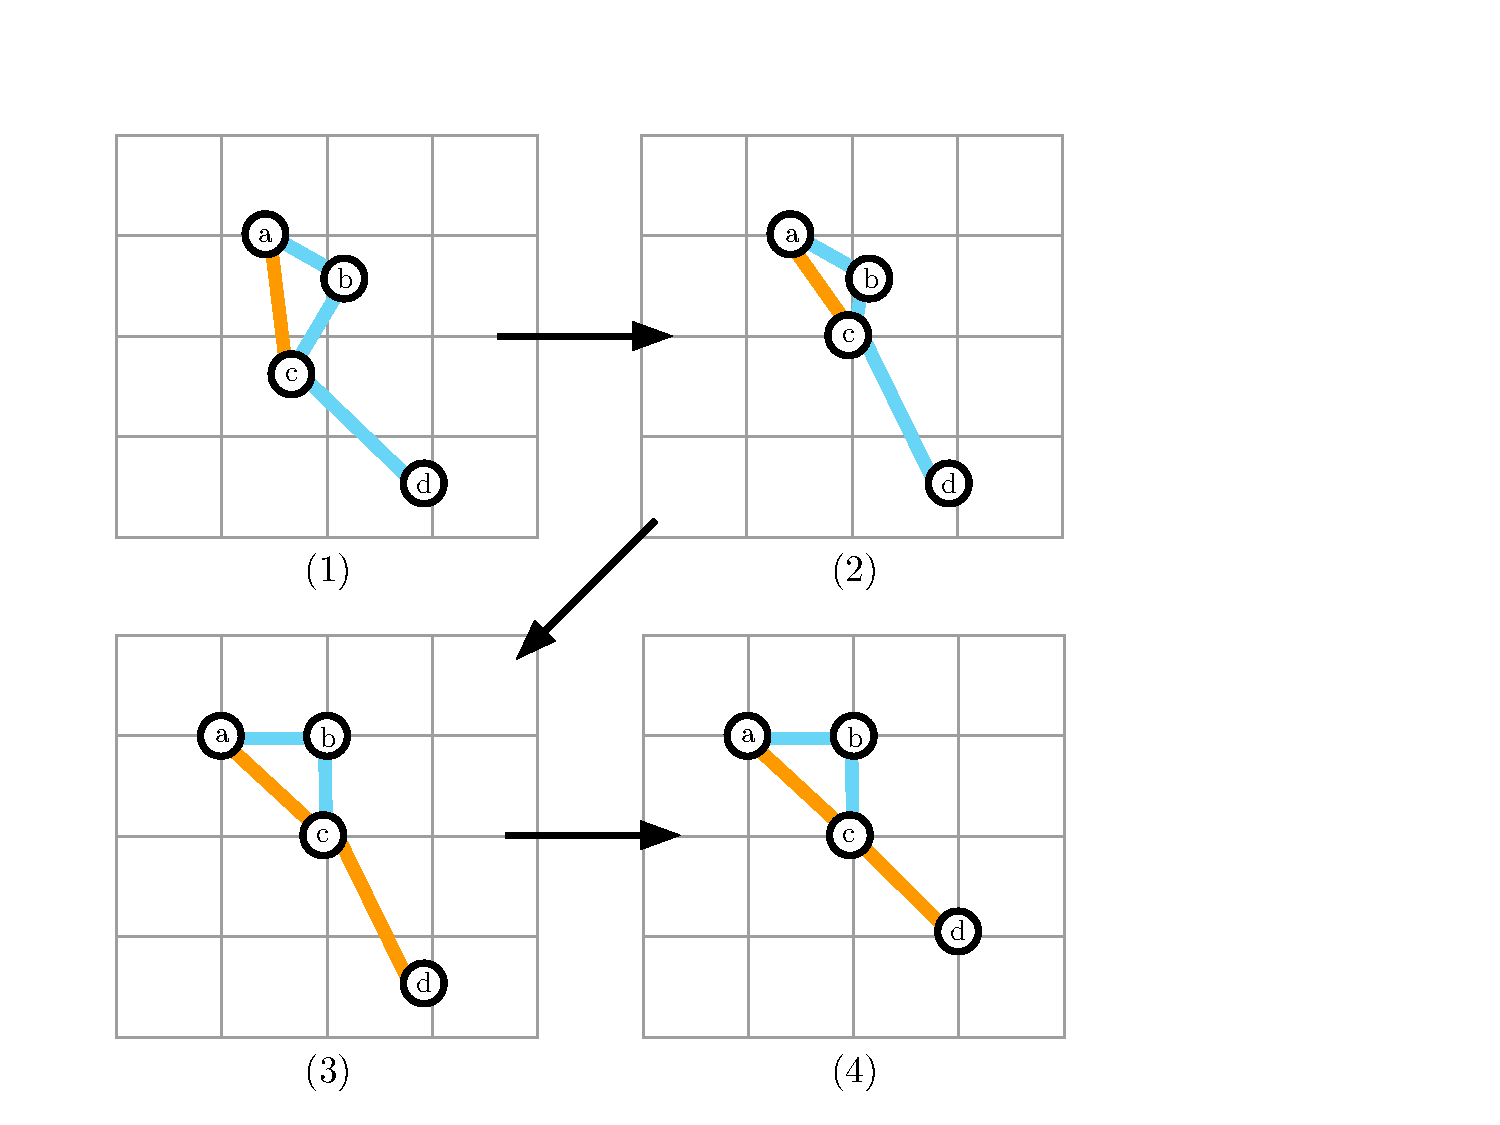
\includegraphics[width=.9\textwidth]{img/implementation/snap.pdf}
	\caption{An example demonstrating the \textit{snap-to-grid} process}
	\label{fig:snap}
\end{figure}

Figure \ref{fig:snap} shows the \textit{snap-to-grid} process applied to a small example. We snap stations in order of descending weight (number of incident edges), as typically the more edges a node is connected to, the more difficult it is to place. In the example, this means station $c$ (with weight 3) is moved first. There is contention for the second move, as both stations $a$ and $b$ have weight two, so we make an arbitrary decision as to which we move first, and the two moves are shown as one step. The final station to move is station $d$, after which we can mark all stations as successfully placed. 

Stations whose nearest intersections are already occupied are left unplaced. This implementation contrasts slightly with \citeauthor{AutomaticMetroMapLayoutThesis}'s approach, where stations are snapped \textit{in order} of Euclidian distance to their nearest intersection, and snapped to the next-nearest if the closest intersection is already occupied. We found this implementation performed poorly for maps with several highly connected nodes, which is a common due to news providers publishing review articles covering many of the lines on the map.

To determine the final station positions, our approach now diverges from \citeauthor{AutomaticMetroMapLayoutThesis}'s into a heuristic method which has been refined for metro maps comprising between 10 and 50 stations. It is vital that metro lines with high affinity have been removed before this stage, or the following process will result in a map where nodes with high weights are occluded.

Although by definition the \textit{snap-to-grid} gives a map near-perfect octilinearity, it can significantly worsen line-straightness, as shown in Figure \ref{fig:aoct}. It would be preferable to have the circled station repositioned as the transformation shows, even though this sacrifices the uniform edge length of the map. We therefore make several passes over each metro line, moving stations to the midpoint of the line between the previous and next neighbouring stations if that line is octilinear.
\begin{figure}[htbp!]
	\centering
	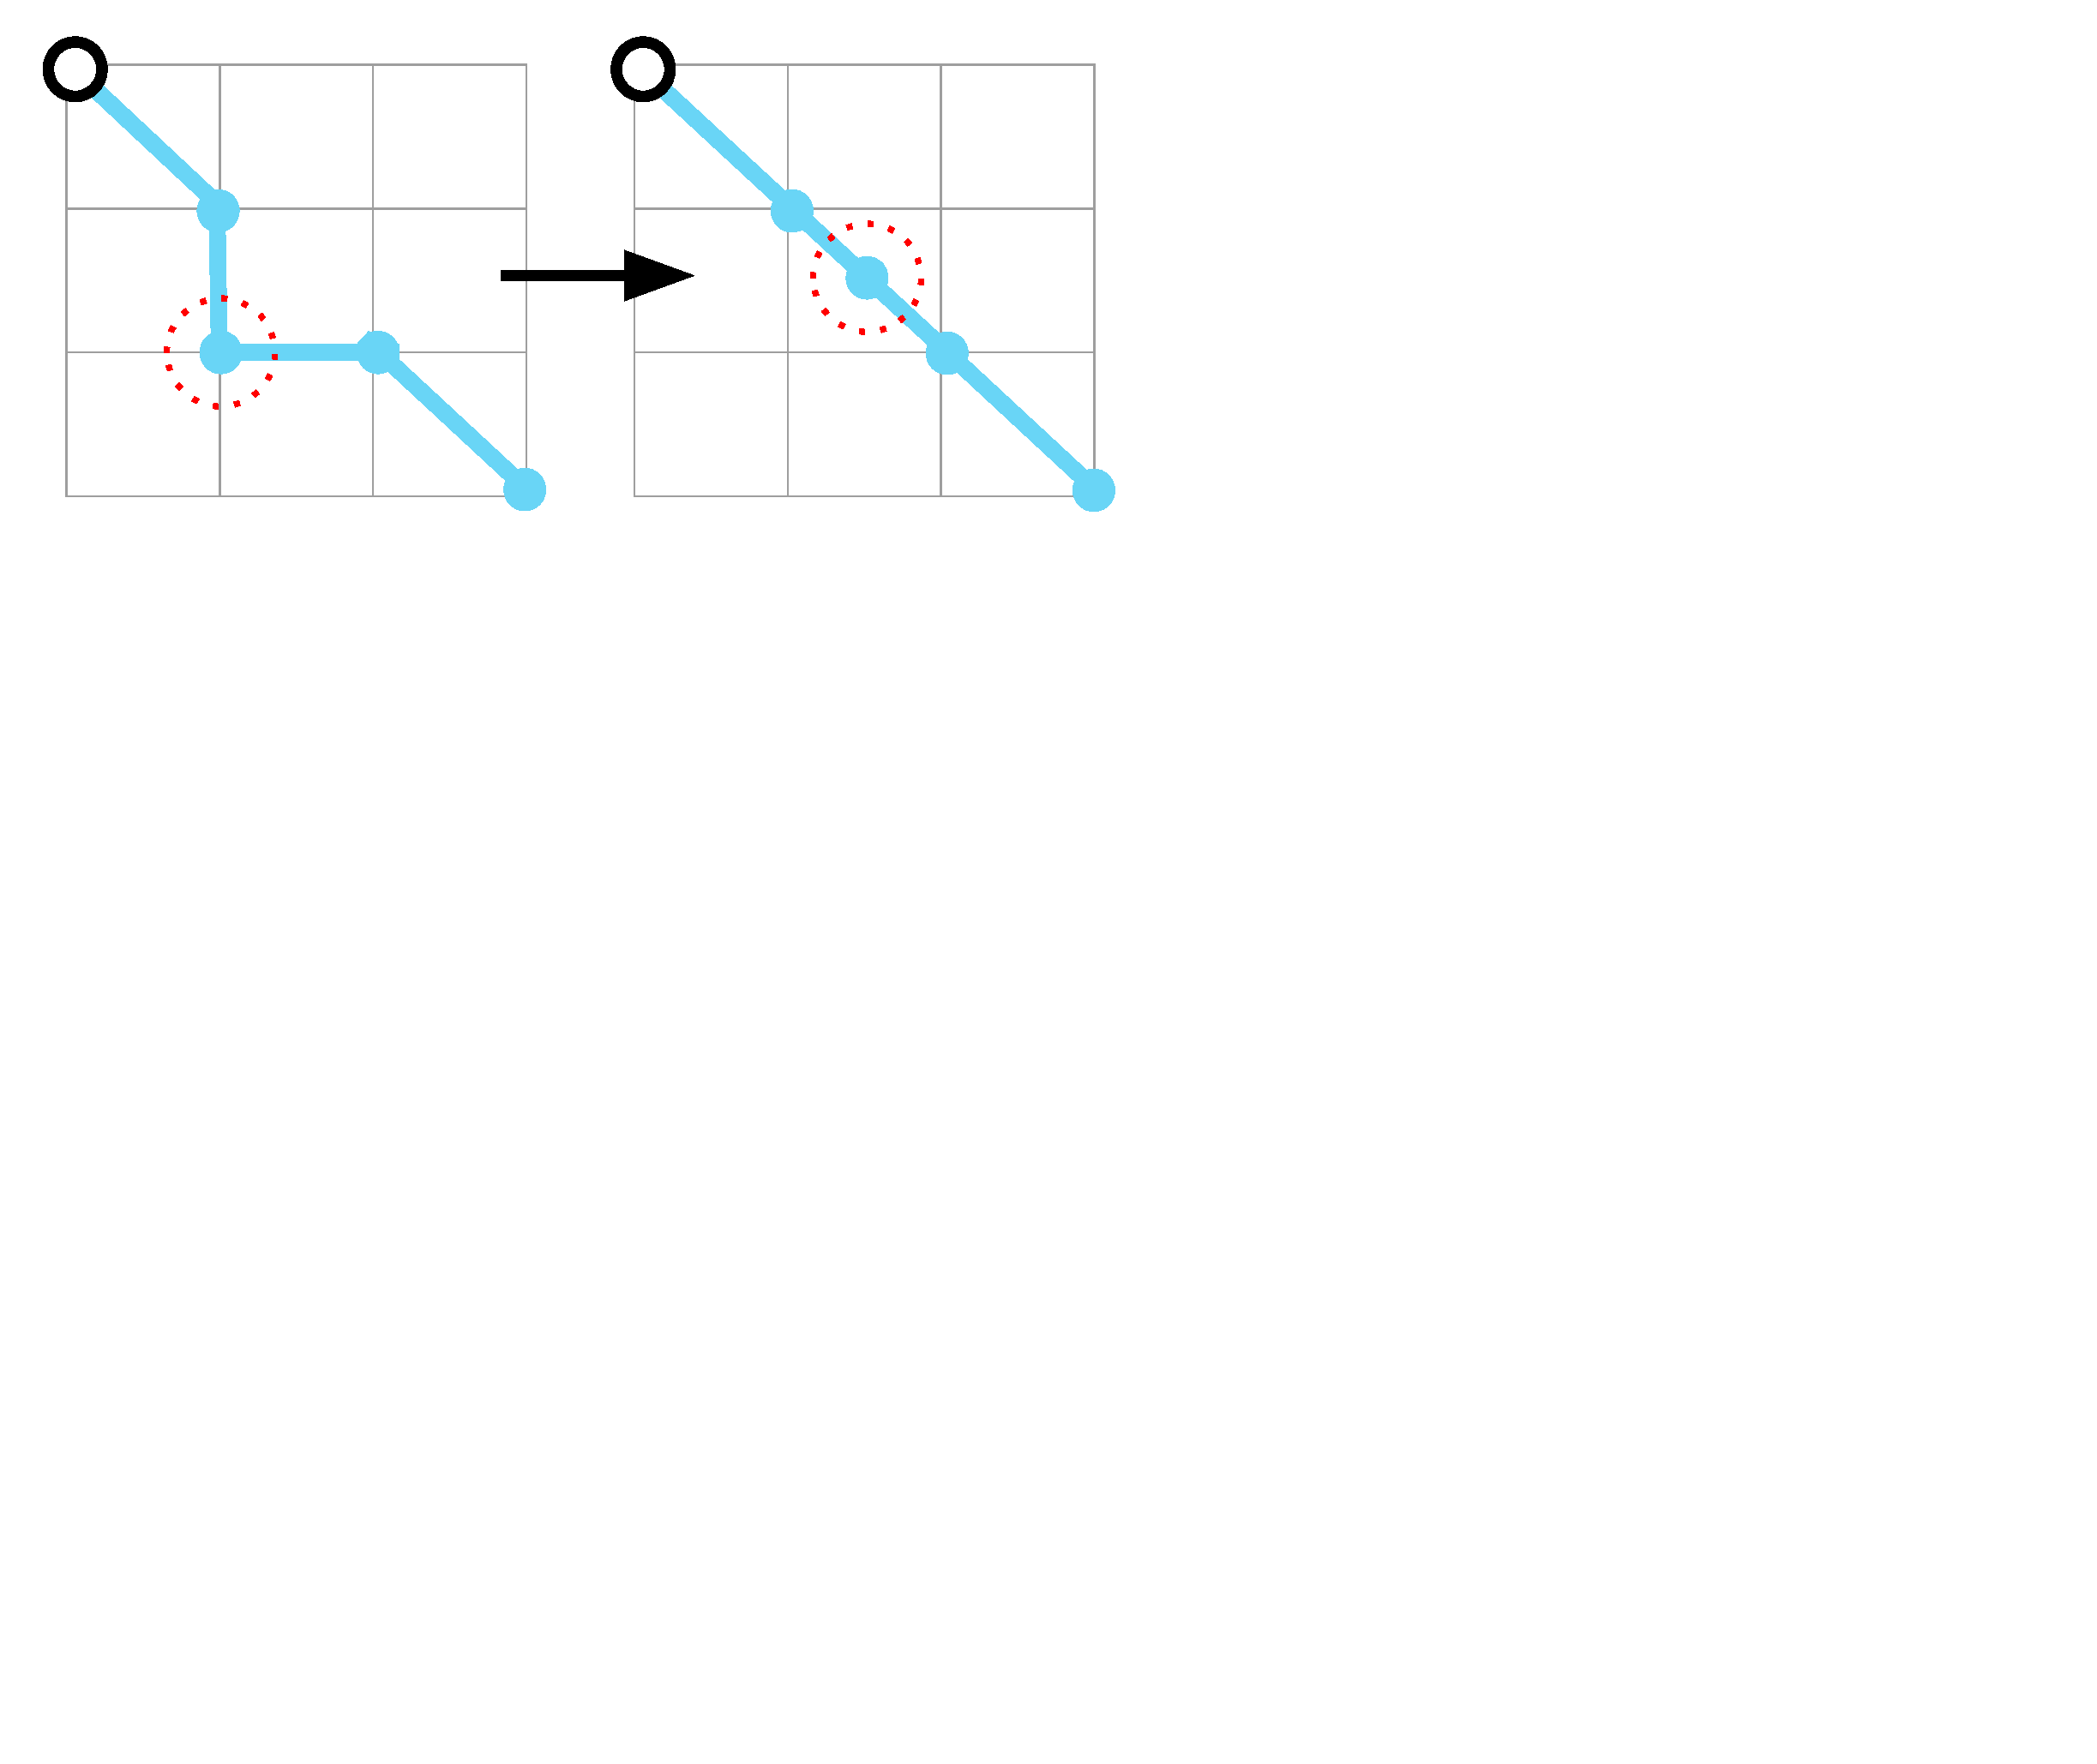
\includegraphics[width=.7\textwidth]{img/implementation/averagingoctilinear.pdf}
	\caption{An octilinear move which compromises the edge-length criterion}
	\label{fig:aoct}
\end{figure}

In addition, a final pass checks for stations which are still unplaced at this point and performs the same midpoint movement regardless of whether the line between the next and previous points is octilinear. This is simply to try and ensure the unplaced point obscures and crosses as few other links as possible in what is most likely a densely packed area of the map. An example of this process is shown in Figure \ref{fig:nonoct}.
\begin{figure}[htbp!]
	\centering
	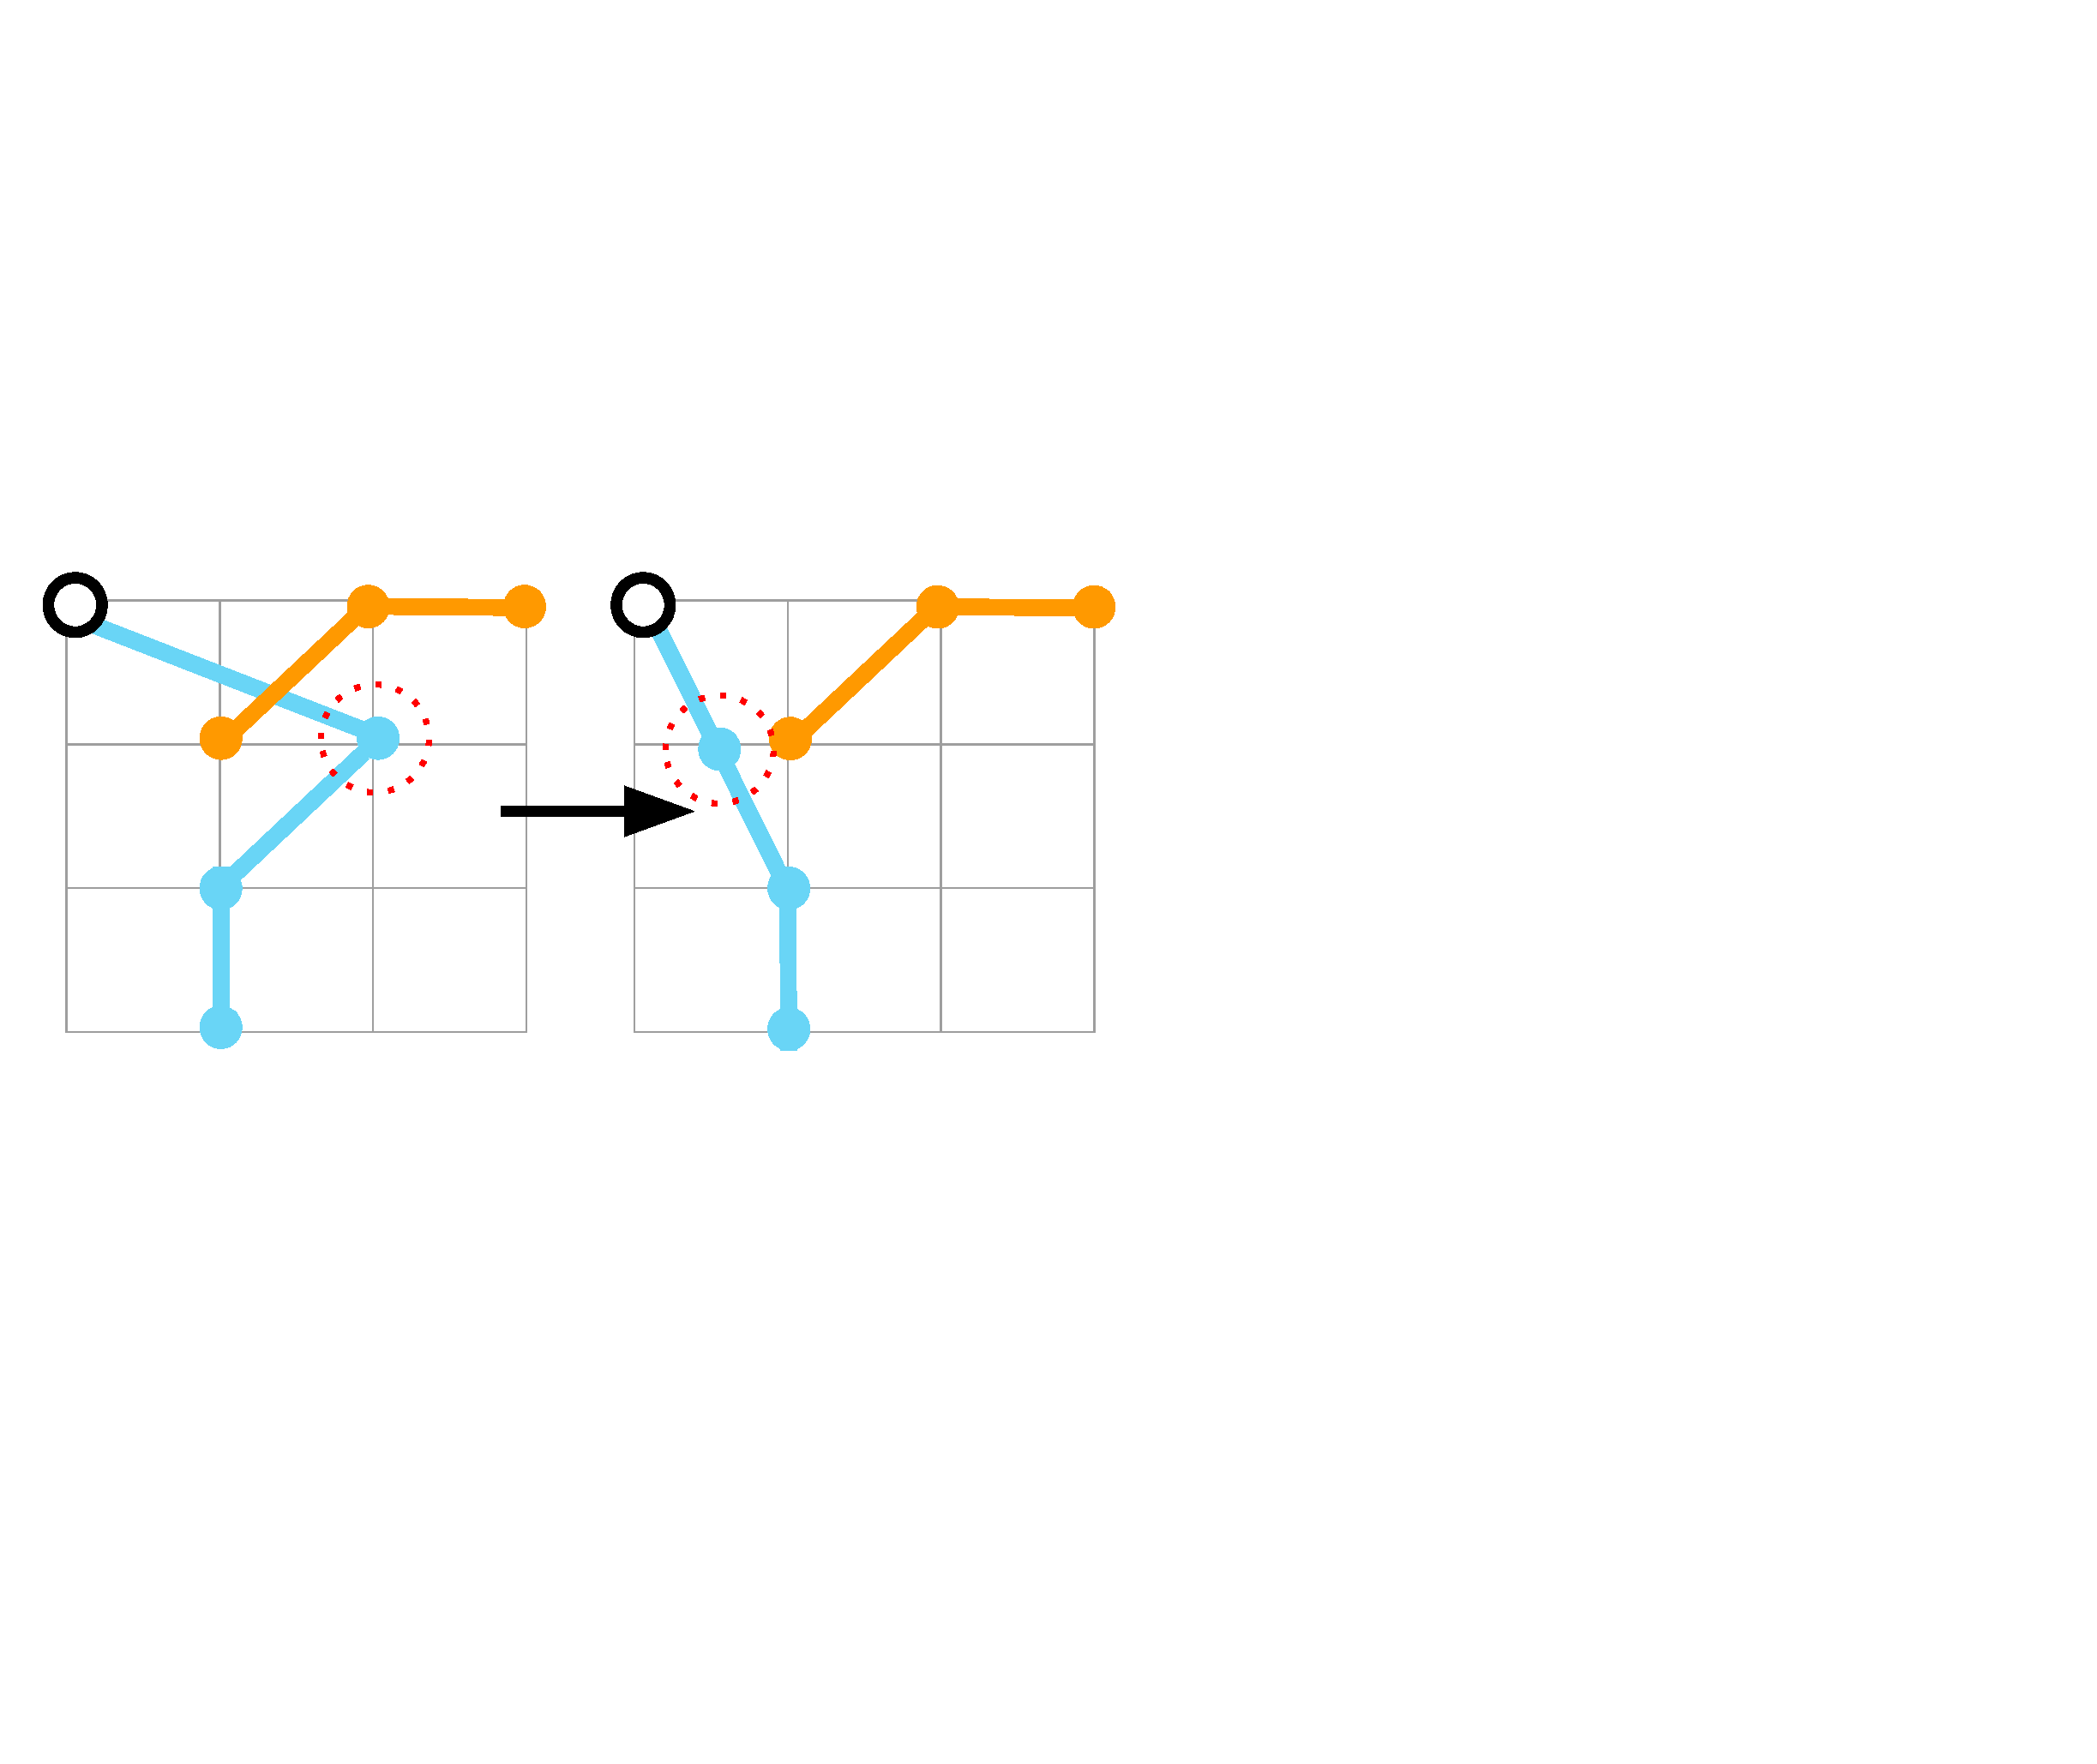
\includegraphics[width=.7\textwidth]{img/implementation/averagingnonoctilinear.pdf}
	\caption{A non-octilinear move of an unplaced station}
	\label{fig:nonoct}
\end{figure}

After the final pass, we recompute octilinearity and line-straightness, and count how many points were left unplaced; i.e. drawn directly on top of another point. If any of the numbers are unsatisfyingly high, the process can be restarted and the randomness of the initial force-direction will result in a different initial embedding.

\section{Summary}

We have given a detailed description of the system's pipeline and the novel transformation of news data from XML elements in an RSS feed to raw text, to parsed keywords, to recognised entities, to elements in a directed graph, to stations on a formatted metro map.

Several unexpected difficulties arose during implementation, in particularly the tradeoffs involved with entity disambiguation in the context of what makes a ``useful'' metro line, and the process of deciding which lines to select between two or more with high affinity. 

However, the most significant challenge of implementation was undoubtedly the process of drawing usable metro maps. The conflict between edge crossings, line-straightness and octilinearity was omnipresent, and the final algorithm still falls into local minima as it is unable to detect the edge crossings. This section of the pipeline would benefit greatly from further work, as it is a significant area of active research in its own right. As the expected datasets for the map are typically small (under 50 stations),  a non-polynomial time algorithm for refining station positions would be feasible in terms of running time, and would doubtless improve the quality of the maps generated.

The results obtained by using the system to generate metro maps for various news corpora are discussed in the next chapter.



\chapter{Results and Discussion}
\label{c:results}
%\section{Feed Extraction}

\section{Article Processing}

\section{Graph Formation}

\section{Graph Placement and Visualisation}

\chapter{Empirical Evaluation}
\label{c:evaluation}
%Typically, information retrieval tools can be evaluated in terms of  accuracy and other quantifiable metrics against a canonical labelled dataset. Our system is less amenable to such evaluation due to the lack of existing datasets. The extensive user study conducted by \cite{GeneratingInformationMaps} evaluated four distinct aspects of their metro map system; (1) Accuracy of the algorithm's document selection in respect to a query; (2) User fact retrieval time; (3) User understanding at a macro level; and (4) task performance of users with a Metro Map versus an unstructured list.

For our system, the first aspect (accuracy of retrieval for queries) is not of interest, because our maps are not query-based or selected from a large fixed corpus with a reasonable likelihood of type II errors.

The second and third, while relevant to our system, do not effectively capture the spirit of its intended purpose. Our metro maps are not designed for search tasks; if a user has a specific question about an article in a metro map, they will most likely still have to open and read the article itself for the answer. The maps exist to help the user form high-level connections between topics and to make sense of those they do not understand. A search task would have to ask artificially simple questions in order for the answers to be derivable using our maps alone, and would therefore not be representative of typical news consumption tasks.

The final aspect is therefore what we chose to focus on. The goal of the experiment is to determine whether the structure of the metro maps alone provides a better overview to news content than a the traditional RSS feed view. We answer this question using \possessivecite{TowardsAnOptimalResolutionToInformationOverload} dimensions of information overload to choose two perspectives to evaluate:

\begin{itemize}
	\item Users' perceptions of \textbf{information quantity}. \par
		Since information overload is based partially on readers' intrinsic estimations of information quantity, we examine the effect that varying information format has on these estimations.
	\item The \textbf{contextual quantity} of our maps, as measured by task performance. \par
		We conduct an experiment similar to that of \cite{scattergather}, measuring the effect of varying information format on the breadth and depth of users' topic recollection.
\end{itemize}

\section{Experimental Hypotheses}

Considering perception and performance as our two separate measures of information overload, we developed the following hypotheses to be tested in two separate experiments:

\begin{hyp}[\ref{hyp:eq:estimation}]
\label{hyp:estimation}
Users' estimates of the number of articles in a metro map are lower than their estimates of the same number of articles when displayed in a list form.
\end{hyp}
\vspace{-0.6cm}
\begin{align*}
	H_{0}(\ref{hyp:estimation}) &: \mu{E_{map}} = \mu{E_{list}} \\
	H_{1}(\ref{hyp:estimation}) &: \mu{E_{map}} < \mu{E_{list}} \numberthis
	\label{hyp:eq:estimation}
\end{align*}

\begin{hyp}[\ref{hyp:eq:index}]
\label{hyp:index}
Users recall a higher number of topics after using a metro map representation than after using the RSS feed list view.
\end{hyp}
\vspace{-0.6cm}
\begin{align*}
	H_{0}(\ref{hyp:index}) &: \mu{T_{map}} = \mu{T_{list}} \\
	H_{1}(\ref{hyp:index}) &: \mu{T_{map}} > \mu{T_{list}} \numberthis
	\label{hyp:eq:index}
\end{align*}

Where $\mu{E}_{map}$ and $\mu{E}_{list}$ are the mean estimate values for the number of articles contained within a map and list respectively, and $\mu{T}_{map}$ and $\mu{T}_{list}$ are the mean number of topics successfully recalled.

Due to the small sample size of the experiment, the null hypothesis was tested at 5\% ($\alpha = 0.05$) significance. 


\section{Experimental Design}

In order to increase the number of subjects participating in each condition and control for individual variances in ability, both experiments were conducted within-groups. With each subject participating in both conditions (\textit{map} and \textit{list}), two corpora of news articles were required. Subjects were therefore assigned to one of four groups, with counterbalancing of the order in which the conditions were conducted (Table \ref{tab:experimentalgroups}.) All four groups contained the same number of participants. \\

\begin{table}[htbp!]
\centering
\begin{tabular}{|r|c|c|}
\hline
  & A, B & B, A\\
\hline
\textit{List}, \textit{Map} & (Group 1) \textit{List} A \textbf{then} \textit{Map} B & (Group 3) \textit{List} B \textbf{then} \textit{Map} A \\
\hline
\textit{Map}, \textit{List} & (Group 2) \textit{Map} A \textbf{then} \textit{List} B & (Group 4) \textit{Map} B \textbf{then} \textit{List} A \\
\hline
\end{tabular}
\caption{Participant Groups} \label{tab:experimentalgroups}
\end{table}

To prevent conscious or subconscious counting by participants during the second condition, subject were exposed to both datasets for 60 seconds, one immediately after another. After exposure to the second set, they were asked to estimate the number of articles in both sets.

\subsection{Planning}





\subsection{Variables}

\subsubsection{Independent Variables}

The independent variable in both experiments is the display modality; a nominal value which is either \textit{metro map} or \textit{list}. Participants will complete the same tasks with both a metro map and a list modality, using a different news corpus for each.

\subsubsection{Dependent Variables}

\begin{itemize}
	\item\textbf{Article Estimate (Hypothesis \ref{hyp:estimation})} \par
		This is the estimate of the number of articles divided by the actual number of articles present, and is measured on a ratio scale, with a perfect estimate being 1.0. 
	\item\textbf{Primary topics (Hypothesis \ref{hyp:index})} \par
		This is the number of `top-level' topics identified in a participant's index which are present in the corpus, measured on a ratio scale.
	\item\textbf{Topic index depth (Hypothesis \ref{hyp:index})} \par
		This is the maximum depth reached in a participant's index, measured on a ratio scale.
	\item\textbf{Total topics (Hypothesis \ref{hyp:index})} \par
		This is the total number of topics identified at all levels in a participant's index which are present in the corpus, measured on a ratio scale.
	\item\textbf{Self-Assessment Manikin (SAM) score (Hypothesis \ref{hyp:index})} \par
		The valence, arousal and dominance experienced by participants after completing Experiment 2.

\end{itemize}

\subsubsection{Control Variables}
There were a number of participant characteristics and other covariates which could confound the results of one or both experiments. The majority of these are controlled for due to all subjects participating in both conditions, or due to our participant selection process, but they are all listed below.

\begin{itemize}
	\item\textbf{Level of formal education} \par
		It was expected that participants' respective levels of formal education may impact their performance, however, as the experiments are within-groups and all of our participants were undertaking the final year of an undergraduate degree, we did not account for this as a covariate.
	\item\textbf{Weekly news consumption time} \par
		It was expected that participants who consume more news on average will perform uniformly better across both conditions, but as subjects participate in both conditions we do not expect to need to account for this as a covariate. This was measured on a discrete scale of hours per week.
	\item\textbf{Past or present use of an RSS feed reader} \par
		As above, it was expected that participants who currently use or have previously used an RSS reeder may perform disproportionally better with the \textit{list} condition than with the \textit{map}. This variable was measured on an ordinal scale of ``Current Usage", ``Previous usage", or ``No usage." This factor was examined as a possible covariate.
	\item\textbf{Topic Familiarity} \par
		Since all subjects participated in both conditions, each subject completed the \textit{metro map} condition with one set of articles and the \textit{list} condition with the other set. The two corpora (A and B) were extracted from the same RSS Feed\footnote{The Guardian, US News, week commencing 20/03/2017.} within the same week, to ensure background knowledge wouldn't confound performance between A and B.
	\item\textbf{Relative complexities of the two corpora} \par
	Although both A and B contained exactly the same number of articles (31), corpus A was significantly more connected, with 39 links; 18\% more edges than corpus B's 33. This factor is discussed more later in the chapter.
\end{itemize}


\subsubsection{Participant Criteria}
All participants recruited for the study were undergraduates between the ages of 20 and 23. They all had perfect or corrected-to-perfect vision and hearing. There were no gender requirements, but the majority of subjects were male.

No participants were excluded on the basis of how much or how little news they consumed on a daily basis. Similarly, although it was recorded whether participants had previously used or currently use an RSS feed reader, this was not used as a selection criterion. 


\section{Methodology}

\section{Results}

Because both experiments were conducted within-groups and every participant was therefore observed twice, observations are not independent, so we use a paired t-test to test the significance of our findings.

\section{Summary}

\chapter{Conclusions}
\label{c:conclusions}
%The following chapter outlines the contributions of this work and the limitations of both our system and evaluation. It also describes extensions which could be developed given additional time, and areas which would benefit from further research.

\section{Summary of Contributions}

This dissertation introduced the first application of the metro map metaphor \citep{GeneratingInformationMaps} to news corpora extracted from user-specified RSS feeds, in order to automatically generate structured topic maps based on current events news. These metro maps serve as an effective comprehension aid to young people in our current digital landscape of news overload; a claim which we are the first to evaluate via direct comparison or our system with a typical RSS feed reader.

Our implementation includes a novel keyword extraction algorithm which performs keyword boosting using a knowledge base for entity disambiguation, and is tuned specifically for extracting entities from current events news. In the subdomain of metro map topology, our method also formalises \textit{Line Coverage} and \textit{Affinity} as an extension to the characteristics defined by \cite{GeneratingInformationMaps}, which can be used to compare the quality of candidate lines during the selection and pruning processes.

Due to the lack of any existing library for positioning or drawing metro maps, further contributions made include recommendations on tuning specific D3.js parameters within a force-directed layout to generate viable starting positions for stations on a metro map, and notes on the implementation of functions to calculate \possessivecite{AutomaticMetroMapLayoutThesis} line straightness and octilinearity criteria in JavaScript. To the best of our knowledge, this is the first application of \citeauthor{AutomaticMetroMapLayoutThesis}'s aesthetic criteria for metro map layout optimisation to non-geospatial maps.

The final contribution of this work is an empirical evaluation of the task performance of young adults using the system. The results of our experiments support our hypothesis that users recall more news topics from a news corpus using our metro maps than after using an unstructured RSS feed reader, and therefore substantiate our recommendations that future efforts to support the contextual linking of news articles should look to visualisation and cartography for direction.

\section{Limitations}

The main limitation of this work is the lack of a formal deterministic algorithm for drawing metro maps, using D3 or otherwise. The approach presented in Section \ref{sec:drawing} is nondeterministic by necessity in order to generate initial starting positions which result in few or no edge crossings, but this process is non-convergent and often results in suboptimal embeddings, the worst cases of which are unusable. 

As a result of this limitation, a significant effort was made to decouple the map drawing process from the other components of the system, such that it could be improved or replaced in future with the only changes required being to the interface at the serialisation stage. While the problem of generating planar embeddings for metro maps is known to be NP-hard, the maps drawn by our system are typically significantly smaller than metro maps which represent real existing transit networks, meaning it would not be unrealistic to use a non-polynomial time algorithm.

A second important limitation of the system is the inability of the graph formation logic to recognised an overly sparse, overly connected, or overly populated map. All three of these properties are easily addressed in theory; an overly sparse graph should trigger a repeat of the keyword extraction process with a larger keyword vector per article, an overly connected graph should trigger a repeat of the same process with a smaller keyword vector per article, and an overly populated map should use both a smaller keyword vector and have its lowest ranking metro lines removed. However, in the given time, it was not possible to implement this logic in the system, resulting in a need to manually tune parameters such as the above during its operation.

In terms of experimental design, the the weaknesses of this work lie in its limited scope. While our user study managed to capture a wide range of news consumption behaviours and attitudes among participants, all participants were students aged 20-23 who were technically proficient. 15 out of the 16 were Computer Science undergraduates, who are typically more familiar with graph theory and therefore more confident interpreting representations of abstract graphs than the general young adult population. This is a limitation which could be addressed by further experiments, as although the system was conceptualised for use by young adults as a result of The \possessivecite{anewmodelfornews} findings, it would have strengthened our conclusions to have evaluated the system in a larger study of both adults adults over the age of 25, and teenagers, especially those from a non-scientific background.

In addition to the lack of participant academic diversity, the scope of our measurement of task performance could also have been extended. The study we conducted was focussed exclusively on recall, but this recall is only one of the six factors identified by \cite{VisuelleKommunikation} as being strengthened by the use of visual metaphors, the others being motivation, the formation of new perspectives, support for learning, focusing of attention, and structuring of communication. It could be argued that the act of creating a topic index also evaluated the structure of participants' communication, but this still leaves four factors remaining.  

A more long-term study could have evaluated whether the daily use of metro maps supported participants' learning and/or increased their motivation to read the news, as these were the two factors identified in Chapter \ref{c:litreview} as the most critical influencers of news fatigue.


\section{Directions for Future Research}

This section outlines areas we consider to be of interest for future work on the basis of this dissertation.

\subsection{Real-Time News Tracking for Automated Collation}

If the system were developed to a stage where no manual tuning was required to prune the candidate metro lines to a level which struck a balance between useful and usable, article collation would a simple process to automate, meaning maps could be automatically generated on a periodic basis with no need for user input.

Web services such as News API \footnote{\url{https://newsapi.org}}, which publish a continual stream of JSON metadata containing live headlines from 72 major worldwide news publishers, are gaining traction as the demand for immediate information increases. Although metro maps have not been designed with live updating in mind, the use of services such as News API could serve as a replacement for specific RSS feeds, removing the major initial parameter of the system.

The key questions posed by the concept of real-time metro maps of news are related to the mechanics of updating, and how stateful the updates should be. Should the publishing of ten new headlines trigger a complete regeneration of the map (which would potentially result in a new set of metro lines) or should metro lines be fixed over a specific period of time? Would users want to be able to `pin' metro lines to indicate that the system should consider this an ongoing topic of interest and always choose it as a candidate?

We suspect that there is a limitation on the usefulness of metro maps when their data is continually updating in real-time due to the structural changes which could occur within the maps, but the core idea of dispensing with specific RSS feeds and simply watching major news outlets for trends is an interesting one. While users may find it beneficial to combatting news fatigue to specify exactly where they want their news to originate from or which topics they want to read about, real-time headlines also take the effort out of specifying feeds for users who are indifferent about the sources of the news they consume.


\subsubsection{Social Media Trending Topics}

In the current information landscape, it is impossible to discuss real-time news publishing without touching on social networks. The evolution of social media websites -- in particular, Twitter -- has been instrumental in the erosion of the dichotomy between news media and social networking websites. The majority of people receive personalised news recommendations every time we open Facebook or Twitter, sometimes without realising that their personal data and browsing histories are being used to construct these recommendations.




\subsection{Verification of News}





\bibliography{bibliography.bib}

\begin{appendices}
\chapter{Full Requirements Specification}
\renewcommand{\thesubsection}{\arabic{subsection}}
\renewcommand{\labelenumi}{\alph{enumi})}
\section{Functional Requirements} \label{sec:freqs}

\subsection{Article Retrieval}
\subsubsection{Description}
The article retrieval component of the system will accept the URL of one or more RSS feeds, collect links to the articles referenced and parse the text of those articles for further processing.
\subsubsection{Functional Requirements}
\begin{enumerate}[F\thesubsection.1]
	\item\label{f1.1}\requirement{The system must accept any standard XML document compliant with the RSS 2.0 specification\footnote{http://cyber.harvard.edu/rss/rss.html}, i.e. it should not be specific to any particular news provider}{High}
	\item\label{f1.2}\requirement{The system must be able to extract a specified number of articles from an RSS feed, in reverse chronological order.}{High}
	\item\label{f1.3}\requirement{The system must be able to download the textual content and/or raw HTML for each article.}{High}
	\item\label{f1.4}\requirement{The system should accept multiple RSS feeds from one or more news provider(s) and merge their content into one collection.}{Medium}
	\item\label{f1.5}\requirement{The system could verify new article URLs against the URLs of imported articles to ensure no articles are duplicated.}{Medium}
\end{enumerate}

\subsection{Keyword Extraction}
\subsubsection{Description}
The keyword extraction stage will tokenise the parsed article text and determine a set of significant keywords for each article individually.
\subsubsection{Functional Requirements}
\begin{enumerate}[F\thesubsection.1]
	\item\label{f2.1}\requirement{The system must tokenise articles in order to perform basic natural language processing such as stop-word extraction and lemmatising.}{High}
	\item\label{f2.2}\requirement{The system must implement a method for keyword extraction, and calculate a corresponding measure of relative importance for each keyword such as tf-idf.}{High}
	\item\label{f2.3}\requirement{The system could attempt to combine keywords it considers equivalent (e.g. \textit{UK} and \textit{United Kingdom}) to form stronger keyword matches between or within articles.}{Medium}
	\item\label{f2.4}\requirement{The system could use external services (e.g. Google's Knowledge Graph API\footnote{http://www.google.com/intl/es419/insidesearch/features/search/knowledge.html}) to query any extracted keywords, in order to gain further insight or perform entity disambiguation \citep{EntityDisambiguationForKnowledgeBasePopulation}.}{Low}
\end{enumerate}

\subsection{Graph Building}
\subsubsection{Description}
This process involves determining a set of corpus keywords from the union of all the articles' keywords to form connected paths of edges (\textit{lines}), and fitting a maximal number of articles into the resulting graph.
\subsubsection{Functional Requirements}
\begin{enumerate}[F\thesubsection.1]
	\item\label{f3.1}\requirement{The system must analyse the keywords extracted from all articles in a corpus to choose a set of the $n$ most significant topics, where $n$ is either predetermined or user-specified.}{High}
	\item\label{f3.2}\requirement{The system must use the extracted topics and the publish dates (which form a natural ordering of nodes) of the articles to form a directed graph, with articles as vertices and common topic storylines as edges.}{High}
	\item\label{f3.3}\requirement{The system should accept a user-specified topic or list of topics to include or exclude from the graph.}{High}
	\item\label{f3.4}\requirement{The system should choose topics which are specific to some but not all articles in the collection, so as to avoid highly correlated topic keywords.}{Medium}
	\item\label{f3.5}\requirement{The system could support exporting generated graphs in a graph description language e.g. DOT\footnote{http://www.graphviz.org/content/dot-language} or GraphML\footnote{http://graphml.graphdrawing.org}.}{Medium}
	\item\label{f3.6}\requirement{The system could attempt to combine keywords to form topics if it considers them highly correlated.}{Medium}
	\item\label{f3.7}\requirement{The system could attempt to maximise the coverage of the topic selection, i.e. maximise the number of articles covered by a given set of keywords.}{Medium}
\end{enumerate}

\subsection{Map Drawing}
\subsubsection{Description}
The visualisation component will generate an interactive visualisation of the graph which can be used to explore the corpus as a whole and drill-down to the individual article level. 
\subsubsection{Functional Requirements}
\begin{enumerate}[F\thesubsection.1]
	\item\label{f4.1}\requirement{The system must provide the capability for users to visualise the graph structures it generates using any HTML5 compliant web browser.}{High}
	\item\label{f4.2}\requirement{Metro lines must each be drawn in a different colour which contrasts that of other lines.}{High}
	\item\label{f4.3}\requirement{The visualisation must include a key mapping metro line names to their colours on the map.}{High}
	\item\label{f4.4}\requirement{Stations must be drawn with common (non-unique) symbols, with a distinction made for interchange stations.}{High}
	\item\label{f4.5}\requirement{The system must provide drill-down details for nodes, e.g. by providing a hyperlink to the original article or embedding static content from each article within the visualisation itself to provide a preview.}{High}
	\item\label{f4.6}\requirement{The maps generated should be readable by ensuring nodes and edges do not overlap with each other where possible.}{Medium}
	\item\label{f4.7}\requirement{In support of \ref{f4.6}, to improve the readability of the map, nodes should not be labelled with article titles.}{Medium}
	\item\label{f4.8}\requirement{The maps generated should adhere (where possible) to the metro map aesthetics defined in \citep{AutomaticMetroMapLayoutThesis, AutomaticMetroMapLayout} to preserve the familiarity of the metaphor.}{Medium}
	\item\label{f4.9}\requirement{The system could allow some degree of interactive customisation which does not change the underlying structure of the graph, such as dragging nodes or changing attributes including colour.}{Low}
\end{enumerate}

\subsection{Storage and Persistence}
\subsubsection{Description}
This component of the system is responsible for saving and importing previously downloaded corpora and reconstructing their graphs.
\subsubsection{Functional Requirements}
\begin{enumerate}[F\thesubsection.1]
	\item\label{nf1.1}\requirement{The system must support the importing/exporting of graph and article data in an intermediate data form, in order to fully reconstruct graphs it had previously created.}{High}
	\item\label{nf1.2}\requirement{By default, the articles collected by each run of the system must be treated as a new corpus so keyword ranking is deterministic for any given feed.}{High}
\end{enumerate}

\section{Nonfunctional Requirements} \label{sec:nfreqs}

\subsection{Security}
The system will not require any kind of authentication to use, and will only stores data which is publicly available. As there are no security regulations which govern its usage, security is not a critical consideration and there are only two associated requirements.
\begin{enumerate}[NF\thesubsection.1]
	\item\label{nf2.1}\requirement{The system will not collect any data during installation and usage without obtaining consent from the user.}{High}
	\item\label{nf2.2}\requirement{The system will not transmit any data which was necessary to collect or generate, including log files, without obtaining explicit consent from the user.}{Medium}
\end{enumerate}

\subsection{Software Quality}

The following list specifies the system's core requirements in terms of portability, source control, testability, usability and documentation. There are no specific performance metric requirements for the system at this stage of its development.

\begin{enumerate}[NF\thesubsection.1]
	\item\label{nf3.1}\requirement{The system must not use any platform-specific libraries, functions or commands.}{High}
	\item\label{nf3.2}\requirement{The system must provide a \texttt{requirements.txt}\footnote{https://pip.readthedocs.io/en/1.1/requirements.html} file or similar, to allow its dependencies to be installed using Pip.}{Medium}
	\item\label{nf3.3}\requirement{The system must be versioned and privately hosted on GitHub.}{High}
	\item\label{nf3.4}\requirement{The implementation of the system should include a severity-based logging facility which writes to a text file, for use during debugging and testing.}{Medium}
	\item\label{nf3.5}\requirement{The system must provide a non-interactive help facility for users.}{High}
	\item\label{nf3.6}\requirement{The system should provide visual feedback during computationally expensive tasks to show task progress, e.g. with loading bars.}{Medium}
\end{enumerate}






\chapter{Implementation Raw Data}
\section{Token/Entity Data}
\begin{longtable}[c]{|l|l|l|}
\caption{Entities as a percentage of total tokens from 40 BBC Politics articles.}\label{tab:entitiestokens}\\
\hline
Tokens & Entities & Entities (\%) \\
\hline\hline\endhead
81     & 7        & 8.64198       \\
129    & 8        & 6.20155       \\
167    & 9        & 5.38922       \\
181    & 15       & 8.28729       \\
252    & 17       & 6.74603       \\
264    & 15       & 5.68182       \\
272    & 11       & 4.04412       \\
275    & 17       & 6.18182       \\
291    & 21       & 7.21649       \\
343    & 22       & 6.41399       \\
349    & 14       & 4.01146       \\
366    & 23       & 6.28415       \\
367    & 28       & 7.62943       \\
367    & 14       & 3.81471       \\
404    & 42       & 10.39604      \\
409    & 40       & 9.77995       \\
413    & 41       & 9.92736       \\
434    & 25       & 5.76037       \\
444    & 20       & 4.5045        \\
453    & 29       & 6.40177       \\
480    & 28       & 5.83333       \\
498    & 41       & 8.23293       \\
503    & 30       & 5.96421       \\
523    & 35       & 6.69216       \\
527    & 17       & 3.22581       \\
536    & 62       & 11.56716      \\
562    & 39       & 6.9395        \\
562    & 32       & 5.69395       \\
571    & 42       & 7.35552       \\
618    & 33       & 5.33981       \\
621    & 38       & 6.11916       \\
674    & 35       & 5.19288       \\
688    & 34       & 4.94186       \\
710    & 63       & 8.87324       \\
722    & 65       & 9.00277       \\
831    & 76       & 9.14561       \\
920    & 51       & 5.54348       \\
987    & 83       & 8.40932       \\
1119   & 52       & 4.64701       \\
1243   & 52       & 4.18343       \\
\hline
\end{longtable}
	
\end{appendices}

\end{document}
